% Options for packages loaded elsewhere
\PassOptionsToPackage{unicode}{hyperref}
\PassOptionsToPackage{hyphens}{url}
%
\documentclass[
  letterpaper,
]{book}

\usepackage{amsmath,amssymb}
\usepackage{iftex}
\ifPDFTeX
  \usepackage[T1]{fontenc}
  \usepackage[utf8]{inputenc}
  \usepackage{textcomp} % provide euro and other symbols
\else % if luatex or xetex
  \usepackage{unicode-math}
  \defaultfontfeatures{Scale=MatchLowercase}
  \defaultfontfeatures[\rmfamily]{Ligatures=TeX,Scale=1}
\fi
\usepackage{lmodern}
\ifPDFTeX\else  
    % xetex/luatex font selection
\fi
% Use upquote if available, for straight quotes in verbatim environments
\IfFileExists{upquote.sty}{\usepackage{upquote}}{}
\IfFileExists{microtype.sty}{% use microtype if available
  \usepackage[]{microtype}
  \UseMicrotypeSet[protrusion]{basicmath} % disable protrusion for tt fonts
}{}
\makeatletter
\@ifundefined{KOMAClassName}{% if non-KOMA class
  \IfFileExists{parskip.sty}{%
    \usepackage{parskip}
  }{% else
    \setlength{\parindent}{0pt}
    \setlength{\parskip}{6pt plus 2pt minus 1pt}}
}{% if KOMA class
  \KOMAoptions{parskip=half}}
\makeatother
\usepackage{xcolor}
\setlength{\emergencystretch}{3em} % prevent overfull lines
\setcounter{secnumdepth}{5}
% Make \paragraph and \subparagraph free-standing
\makeatletter
\ifx\paragraph\undefined\else
  \let\oldparagraph\paragraph
  \renewcommand{\paragraph}{
    \@ifstar
      \xxxParagraphStar
      \xxxParagraphNoStar
  }
  \newcommand{\xxxParagraphStar}[1]{\oldparagraph*{#1}\mbox{}}
  \newcommand{\xxxParagraphNoStar}[1]{\oldparagraph{#1}\mbox{}}
\fi
\ifx\subparagraph\undefined\else
  \let\oldsubparagraph\subparagraph
  \renewcommand{\subparagraph}{
    \@ifstar
      \xxxSubParagraphStar
      \xxxSubParagraphNoStar
  }
  \newcommand{\xxxSubParagraphStar}[1]{\oldsubparagraph*{#1}\mbox{}}
  \newcommand{\xxxSubParagraphNoStar}[1]{\oldsubparagraph{#1}\mbox{}}
\fi
\makeatother

\usepackage{color}
\usepackage{fancyvrb}
\newcommand{\VerbBar}{|}
\newcommand{\VERB}{\Verb[commandchars=\\\{\}]}
\DefineVerbatimEnvironment{Highlighting}{Verbatim}{commandchars=\\\{\}}
% Add ',fontsize=\small' for more characters per line
\usepackage{framed}
\definecolor{shadecolor}{RGB}{248,248,248}
\newenvironment{Shaded}{\begin{snugshade}}{\end{snugshade}}
\newcommand{\AlertTok}[1]{\textcolor[rgb]{0.94,0.16,0.16}{#1}}
\newcommand{\AnnotationTok}[1]{\textcolor[rgb]{0.56,0.35,0.01}{\textbf{\textit{#1}}}}
\newcommand{\AttributeTok}[1]{\textcolor[rgb]{0.13,0.29,0.53}{#1}}
\newcommand{\BaseNTok}[1]{\textcolor[rgb]{0.00,0.00,0.81}{#1}}
\newcommand{\BuiltInTok}[1]{#1}
\newcommand{\CharTok}[1]{\textcolor[rgb]{0.31,0.60,0.02}{#1}}
\newcommand{\CommentTok}[1]{\textcolor[rgb]{0.56,0.35,0.01}{\textit{#1}}}
\newcommand{\CommentVarTok}[1]{\textcolor[rgb]{0.56,0.35,0.01}{\textbf{\textit{#1}}}}
\newcommand{\ConstantTok}[1]{\textcolor[rgb]{0.56,0.35,0.01}{#1}}
\newcommand{\ControlFlowTok}[1]{\textcolor[rgb]{0.13,0.29,0.53}{\textbf{#1}}}
\newcommand{\DataTypeTok}[1]{\textcolor[rgb]{0.13,0.29,0.53}{#1}}
\newcommand{\DecValTok}[1]{\textcolor[rgb]{0.00,0.00,0.81}{#1}}
\newcommand{\DocumentationTok}[1]{\textcolor[rgb]{0.56,0.35,0.01}{\textbf{\textit{#1}}}}
\newcommand{\ErrorTok}[1]{\textcolor[rgb]{0.64,0.00,0.00}{\textbf{#1}}}
\newcommand{\ExtensionTok}[1]{#1}
\newcommand{\FloatTok}[1]{\textcolor[rgb]{0.00,0.00,0.81}{#1}}
\newcommand{\FunctionTok}[1]{\textcolor[rgb]{0.13,0.29,0.53}{\textbf{#1}}}
\newcommand{\ImportTok}[1]{#1}
\newcommand{\InformationTok}[1]{\textcolor[rgb]{0.56,0.35,0.01}{\textbf{\textit{#1}}}}
\newcommand{\KeywordTok}[1]{\textcolor[rgb]{0.13,0.29,0.53}{\textbf{#1}}}
\newcommand{\NormalTok}[1]{#1}
\newcommand{\OperatorTok}[1]{\textcolor[rgb]{0.81,0.36,0.00}{\textbf{#1}}}
\newcommand{\OtherTok}[1]{\textcolor[rgb]{0.56,0.35,0.01}{#1}}
\newcommand{\PreprocessorTok}[1]{\textcolor[rgb]{0.56,0.35,0.01}{\textit{#1}}}
\newcommand{\RegionMarkerTok}[1]{#1}
\newcommand{\SpecialCharTok}[1]{\textcolor[rgb]{0.81,0.36,0.00}{\textbf{#1}}}
\newcommand{\SpecialStringTok}[1]{\textcolor[rgb]{0.31,0.60,0.02}{#1}}
\newcommand{\StringTok}[1]{\textcolor[rgb]{0.31,0.60,0.02}{#1}}
\newcommand{\VariableTok}[1]{\textcolor[rgb]{0.00,0.00,0.00}{#1}}
\newcommand{\VerbatimStringTok}[1]{\textcolor[rgb]{0.31,0.60,0.02}{#1}}
\newcommand{\WarningTok}[1]{\textcolor[rgb]{0.56,0.35,0.01}{\textbf{\textit{#1}}}}

\providecommand{\tightlist}{%
  \setlength{\itemsep}{0pt}\setlength{\parskip}{0pt}}\usepackage{longtable,booktabs,array}
\usepackage{calc} % for calculating minipage widths
% Correct order of tables after \paragraph or \subparagraph
\usepackage{etoolbox}
\makeatletter
\patchcmd\longtable{\par}{\if@noskipsec\mbox{}\fi\par}{}{}
\makeatother
% Allow footnotes in longtable head/foot
\IfFileExists{footnotehyper.sty}{\usepackage{footnotehyper}}{\usepackage{footnote}}
\makesavenoteenv{longtable}
\usepackage{graphicx}
\makeatletter
\newsavebox\pandoc@box
\newcommand*\pandocbounded[1]{% scales image to fit in text height/width
  \sbox\pandoc@box{#1}%
  \Gscale@div\@tempa{\textheight}{\dimexpr\ht\pandoc@box+\dp\pandoc@box\relax}%
  \Gscale@div\@tempb{\linewidth}{\wd\pandoc@box}%
  \ifdim\@tempb\p@<\@tempa\p@\let\@tempa\@tempb\fi% select the smaller of both
  \ifdim\@tempa\p@<\p@\scalebox{\@tempa}{\usebox\pandoc@box}%
  \else\usebox{\pandoc@box}%
  \fi%
}
% Set default figure placement to htbp
\def\fps@figure{htbp}
\makeatother
% definitions for citeproc citations
\NewDocumentCommand\citeproctext{}{}
\NewDocumentCommand\citeproc{mm}{%
  \begingroup\def\citeproctext{#2}\cite{#1}\endgroup}
\makeatletter
 % allow citations to break across lines
 \let\@cite@ofmt\@firstofone
 % avoid brackets around text for \cite:
 \def\@biblabel#1{}
 \def\@cite#1#2{{#1\if@tempswa , #2\fi}}
\makeatother
\newlength{\cslhangindent}
\setlength{\cslhangindent}{1.5em}
\newlength{\csllabelwidth}
\setlength{\csllabelwidth}{3em}
\newenvironment{CSLReferences}[2] % #1 hanging-indent, #2 entry-spacing
 {\begin{list}{}{%
  \setlength{\itemindent}{0pt}
  \setlength{\leftmargin}{0pt}
  \setlength{\parsep}{0pt}
  % turn on hanging indent if param 1 is 1
  \ifodd #1
   \setlength{\leftmargin}{\cslhangindent}
   \setlength{\itemindent}{-1\cslhangindent}
  \fi
  % set entry spacing
  \setlength{\itemsep}{#2\baselineskip}}}
 {\end{list}}
\usepackage{calc}
\newcommand{\CSLBlock}[1]{\hfill\break\parbox[t]{\linewidth}{\strut\ignorespaces#1\strut}}
\newcommand{\CSLLeftMargin}[1]{\parbox[t]{\csllabelwidth}{\strut#1\strut}}
\newcommand{\CSLRightInline}[1]{\parbox[t]{\linewidth - \csllabelwidth}{\strut#1\strut}}
\newcommand{\CSLIndent}[1]{\hspace{\cslhangindent}#1}

\usepackage{booktabs}
\usepackage{longtable}
\usepackage{array}
\usepackage{multirow}
\usepackage{wrapfig}
\usepackage{float}
\usepackage{colortbl}
\usepackage{pdflscape}
\usepackage{tabu}
\usepackage{threeparttable}
\usepackage{threeparttablex}
\usepackage[normalem]{ulem}
\usepackage{makecell}
\usepackage{xcolor}
\makeatletter
\@ifpackageloaded{tcolorbox}{}{\usepackage[skins,breakable]{tcolorbox}}
\@ifpackageloaded{fontawesome5}{}{\usepackage{fontawesome5}}
\definecolor{quarto-callout-color}{HTML}{909090}
\definecolor{quarto-callout-note-color}{HTML}{0758E5}
\definecolor{quarto-callout-important-color}{HTML}{CC1914}
\definecolor{quarto-callout-warning-color}{HTML}{EB9113}
\definecolor{quarto-callout-tip-color}{HTML}{00A047}
\definecolor{quarto-callout-caution-color}{HTML}{FC5300}
\definecolor{quarto-callout-color-frame}{HTML}{acacac}
\definecolor{quarto-callout-note-color-frame}{HTML}{4582ec}
\definecolor{quarto-callout-important-color-frame}{HTML}{d9534f}
\definecolor{quarto-callout-warning-color-frame}{HTML}{f0ad4e}
\definecolor{quarto-callout-tip-color-frame}{HTML}{02b875}
\definecolor{quarto-callout-caution-color-frame}{HTML}{fd7e14}
\makeatother
\makeatletter
\@ifpackageloaded{bookmark}{}{\usepackage{bookmark}}
\makeatother
\makeatletter
\@ifpackageloaded{caption}{}{\usepackage{caption}}
\AtBeginDocument{%
\ifdefined\contentsname
  \renewcommand*\contentsname{Table of contents}
\else
  \newcommand\contentsname{Table of contents}
\fi
\ifdefined\listfigurename
  \renewcommand*\listfigurename{List of Figures}
\else
  \newcommand\listfigurename{List of Figures}
\fi
\ifdefined\listtablename
  \renewcommand*\listtablename{List of Tables}
\else
  \newcommand\listtablename{List of Tables}
\fi
\ifdefined\figurename
  \renewcommand*\figurename{Figure}
\else
  \newcommand\figurename{Figure}
\fi
\ifdefined\tablename
  \renewcommand*\tablename{Table}
\else
  \newcommand\tablename{Table}
\fi
}
\@ifpackageloaded{float}{}{\usepackage{float}}
\floatstyle{ruled}
\@ifundefined{c@chapter}{\newfloat{codelisting}{h}{lop}}{\newfloat{codelisting}{h}{lop}[chapter]}
\floatname{codelisting}{Listing}
\newcommand*\listoflistings{\listof{codelisting}{List of Listings}}
\makeatother
\makeatletter
\makeatother
\makeatletter
\@ifpackageloaded{caption}{}{\usepackage{caption}}
\@ifpackageloaded{subcaption}{}{\usepackage{subcaption}}
\makeatother
\makeatletter
\@ifpackageloaded{sidenotes}{}{\usepackage{sidenotes}}
\@ifpackageloaded{marginnote}{}{\usepackage{marginnote}}
\makeatother

\usepackage{bookmark}

\IfFileExists{xurl.sty}{\usepackage{xurl}}{} % add URL line breaks if available
\urlstyle{same} % disable monospaced font for URLs
\hypersetup{
  pdftitle={STA2020 ANOVA Notes},
  pdfauthor={Ané Cloete},
  hidelinks,
  pdfcreator={LaTeX via pandoc}}


\title{STA2020 ANOVA Notes}
\author{Ané Cloete}
\date{}

\begin{document}
\frontmatter
\maketitle

\renewcommand*\contentsname{Table of contents}
{
\setcounter{tocdepth}{2}
\tableofcontents
}

\mainmatter
\bookmarksetup{startatroot}

\chapter*{Preface}\label{preface}
\addcontentsline{toc}{chapter}{Preface}

\markboth{Preface}{Preface}

\emph{Welcome to the Experimental Design and ANOVA section of STA2020.}

This book is not an exhaustive guide to designing experiments or
conducting ANOVA. Instead, it has been tailored specifically to align
with the learning outcomes and methods covered in STA2020.

This module consists of four main sections:

\begin{enumerate}
\def\labelenumi{\arabic{enumi}.}
\tightlist
\item
  Experimental Design
\item
  Completely Randomized Designs
\item
  Randomized Complete Block Designs
\item
  Factorial Experiments
\end{enumerate}

The first two chapters lay the groundwork for the module. Once you grasp
these concepts, the remaining sections should be easier to follow.
Before diving into these topics, there are two preliminary sections:

\begin{enumerate}
\def\labelenumi{\arabic{enumi}.}
\tightlist
\item
  A brief introduction to statistical modeling
\item
  A guide to hypothesis testing
\end{enumerate}

I encourage you to read through these first, as they provide essential
context for the rest of the material.

Throughout the book, you will find R code presented in chunks like this:

\begin{Shaded}
\begin{Highlighting}[]
\NormalTok{x }\OtherTok{\textless{}{-}} \FunctionTok{c}\NormalTok{(}\DecValTok{1}\NormalTok{,}\DecValTok{2}\NormalTok{,}\DecValTok{3}\NormalTok{,}\DecValTok{4}\NormalTok{,}\DecValTok{5}\NormalTok{)}
\FunctionTok{mean}\NormalTok{(x) }\CommentTok{\# Computes the mean of a set of numbers  }
\end{Highlighting}
\end{Shaded}

\begin{verbatim}
[1] 3
\end{verbatim}

R is consistently used to visualize, illustrate, and demonstrate key
methods and concepts. Running the code yourself will greatly enhance
your understanding, so I encourage you to do so.

\begin{quote}
Some parts of these notes have been adapted from the STA1007 notes,
authored by Dr.~Res Altwegg and Dr.~Birgit Erni, as well as from various
textbooks.
\end{quote}

\bookmarksetup{startatroot}

\chapter*{Statistical Modelling}\label{statistical-modelling}
\addcontentsline{toc}{chapter}{Statistical Modelling}

\markboth{Statistical Modelling}{Statistical Modelling}

\section*{What is a Model?}\label{what-is-a-model}
\addcontentsline{toc}{section}{What is a Model?}

\markright{What is a Model?}

A \textbf{statistical model} is a mathematical representation of how
data is generated. It describes the relationship between observed data
and underlying factors (parameters) while accounting for random
variation. Suppose that we are interested in estimating the age of a
tree from its stem diameter. To do this we need to know by how much the
stem diameter increases per year. We could describe this relationship or
process as follows:

\[D = \alpha + \beta \times Age\] describing a linear increase of
diameter with age. Once we have a good idea of how fast diameter
increases with age (β) we can predict diameter from age. The
(mathematical) model above is a very simple representation of this
process with only two parameters, the intercept and the growth rate.

With the chosen parameter values, diameter increases linearly with age.
Of course, this model is not realistic except for special situations but
it gives us powerful insights. In reality we don't know \(\beta\), but
usually need to estimate it from data. Also, not every tree grows
equally fast, because of environmental and individual differences
between trees. We can accept that the above is a simple model for the
average behaviour of a tree, but to capture variability between trees
(because of variability between environmental conditions from tree to
tree, variability between individual trees, measurement error), we add
an error term.

\[D = \alpha + \beta \times Age_i + e_i\]

The response that we observe is then described by an average behaviour,
but the actual observed value will vary around this average. To
summarise, the statistical model has a stochastic component which
captures variability in the response that cannot be explained by the
deterministic part of the model. Another distinguishing feature of
statistical modelling is that we obtain estimates of the parameter
values from the data, e.g.~by fitting a line to the observations,
i.e.~we learn from data.

\section*{More generally}\label{more-generally}
\addcontentsline{toc}{section}{More generally}

\markright{More generally}

Statistical models are not perfect predictors of the data, rather they
attempt to describe the ``central tendency'' of the observations. To get
to the actual observed value some deviation from the central tendency
needs to added (i.e.~error). Such models typically have the following
the form:

\[
\text{Observed Response} = \text{Model Predicted Response} + \text{Error}
\]

Mathematically this can be stated as:

\[Y = \hat{Y} + e\]

A simple example of a statistical model you may have encountered is the
\textbf{mean} as a predictor. Suppose you measure the number of
customers entering two stores over 20 days. The observed counts for each
store fluctuate daily, but you may want to summarize the data using the
average number of customers.

For each store \(i\), a basic statistical model for these observations
would be:

\[
Y_{ij} = \mu_i + e_{ij}
\]

where:

\begin{itemize}
\tightlist
\item
  \(Y_{ij}\) is the number of customers observed on day \(j\) at store
  1,
\item
  \(\mu_i\) is the true mean number of customers at store \(i\),
\item
  \(e_{ij}\) is the error term, representing deviations from the mean.
\end{itemize}

The error term \(e_{ij}\) accounts for day-to-day fluctuations that
cause the actual number of customers to vary around the mean. Below this
data is simulated and plotted, with the model overlain. The black line
is the mean and the red dashed line represents the error for one
observation, i.e.~deviation from the fitted model response, in this case
the mean.

\begin{Shaded}
\begin{Highlighting}[]
\NormalTok{store1 }\OtherTok{\textless{}{-}} \FunctionTok{rpois}\NormalTok{(}\DecValTok{20}\NormalTok{, }\DecValTok{50}\NormalTok{)}
\NormalTok{store2 }\OtherTok{\textless{}{-}} \FunctionTok{rpois}\NormalTok{(}\DecValTok{20}\NormalTok{, }\DecValTok{15}\NormalTok{)}
\NormalTok{storedata }\OtherTok{\textless{}{-}} \FunctionTok{data.frame}\NormalTok{(}\AttributeTok{numcust =} \FunctionTok{c}\NormalTok{(store1, store2),}
                        \AttributeTok{store =} \FunctionTok{factor}\NormalTok{(}\FunctionTok{rep}\NormalTok{(}\FunctionTok{c}\NormalTok{(}\StringTok{"Store 1"}\NormalTok{, }\StringTok{"Store 2"}\NormalTok{), }\AttributeTok{each =} \DecValTok{20}\NormalTok{)))}

\FunctionTok{stripchart}\NormalTok{(numcust }\SpecialCharTok{\textasciitilde{}}\NormalTok{ store, }\AttributeTok{data =}\NormalTok{ storedata,}
           \AttributeTok{method =} \StringTok{"jitter"}\NormalTok{, }\AttributeTok{pch =} \DecValTok{16}\NormalTok{, }\AttributeTok{col =} \FunctionTok{c}\NormalTok{(}\StringTok{"deepskyblue"}\NormalTok{, }\StringTok{"orange"}\NormalTok{),}
           \AttributeTok{vertical =} \ConstantTok{TRUE}\NormalTok{, }\AttributeTok{main =} \StringTok{"Customer Counts per Store"}\NormalTok{,}
           \AttributeTok{xlab =} \StringTok{"Store"}\NormalTok{, }\AttributeTok{ylab =} \StringTok{"Number of Customers"}\NormalTok{)}
\NormalTok{means }\OtherTok{\textless{}{-}} \FunctionTok{tapply}\NormalTok{(storedata}\SpecialCharTok{$}\NormalTok{numcust, storedata}\SpecialCharTok{$}\NormalTok{store, mean)}
\FunctionTok{segments}\NormalTok{(}\AttributeTok{x0 =} \DecValTok{1}\SpecialCharTok{:}\DecValTok{2}\SpecialCharTok{{-}} \FloatTok{0.1}\NormalTok{, }\AttributeTok{x1 =} \DecValTok{1}\SpecialCharTok{:}\DecValTok{2} \SpecialCharTok{+} \FloatTok{0.1}\NormalTok{, }\AttributeTok{y0 =}\NormalTok{ means, }\AttributeTok{y1 =}\NormalTok{ means, }\AttributeTok{lwd =} \DecValTok{3}\NormalTok{, }\AttributeTok{col =} \StringTok{"black"}\NormalTok{) }
\NormalTok{min\_count }\OtherTok{\textless{}{-}} \FunctionTok{min}\NormalTok{(storedata}\SpecialCharTok{$}\NormalTok{numcust[storedata}\SpecialCharTok{$}\NormalTok{store }\SpecialCharTok{==} \StringTok{"Store 1"}\NormalTok{])}
\NormalTok{min\_x }\OtherTok{\textless{}{-}} \FunctionTok{jitter}\NormalTok{(}\FunctionTok{rep}\NormalTok{(}\DecValTok{1}\NormalTok{, }\FunctionTok{sum}\NormalTok{(storedata}\SpecialCharTok{$}\NormalTok{numcust }\SpecialCharTok{==}\NormalTok{ min\_count))) }
\FunctionTok{points}\NormalTok{(min\_x, min\_count, }\AttributeTok{col =} \StringTok{"red"}\NormalTok{, }\AttributeTok{pch =} \DecValTok{16}\NormalTok{, }\AttributeTok{cex =} \FloatTok{1.2}\NormalTok{) }
\FunctionTok{segments}\NormalTok{(}\AttributeTok{x0 =}\NormalTok{ min\_x, }\AttributeTok{x1 =}\NormalTok{ min\_x, }\AttributeTok{y0 =}\NormalTok{ min\_count, }\AttributeTok{y1 =}\NormalTok{ means[}\StringTok{"Store 1"}\NormalTok{], }\AttributeTok{col =} \StringTok{"red"}\NormalTok{, }\AttributeTok{lwd =} \DecValTok{2}\NormalTok{, }\AttributeTok{lty =} \DecValTok{2}\NormalTok{)}
\end{Highlighting}
\end{Shaded}

\pandocbounded{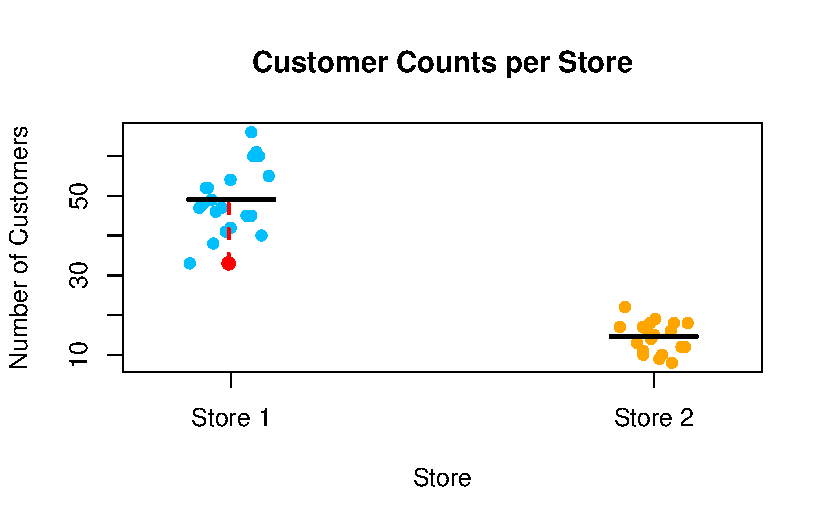
\includegraphics[keepaspectratio]{00_ModelConcepts_files/figure-pdf/unnamed-chunk-1-1.pdf}}

Another basic example of this structure is a \textbf{linear regression
model}:

\[
Y_i = \beta_0 + \beta_1 X_i + e_i
\]

where:

\begin{itemize}
\tightlist
\item
  \(Y_i\) is the observed response,
\item
  \(\beta_0\) and \(\beta_1\) are unknown parameters representing the
  intercept and slope,
\item
  \(X_i\) is the predictor variable,
\item
  \(e_i\) is the random error term.
\end{itemize}

\begin{Shaded}
\begin{Highlighting}[]
\CommentTok{\# Generate random x values and error term}
\FunctionTok{set.seed}\NormalTok{(}\DecValTok{123}\NormalTok{)  }\CommentTok{\# Ensures reproducibility}
\NormalTok{x }\OtherTok{\textless{}{-}} \FunctionTok{rnorm}\NormalTok{(}\DecValTok{35}\NormalTok{, }\AttributeTok{mean =} \DecValTok{35}\NormalTok{, }\AttributeTok{sd =} \DecValTok{5}\NormalTok{)}
\NormalTok{error }\OtherTok{\textless{}{-}} \FunctionTok{rnorm}\NormalTok{(}\DecValTok{35}\NormalTok{, }\AttributeTok{mean =} \DecValTok{0}\NormalTok{, }\AttributeTok{sd =} \DecValTok{5}\NormalTok{)}

\CommentTok{\# Define true model parameters}
\NormalTok{beta0 }\OtherTok{\textless{}{-}} \DecValTok{2}
\NormalTok{beta1 }\OtherTok{\textless{}{-}} \FloatTok{1.5}

\CommentTok{\# Generate y values based on the regression model}
\NormalTok{y }\OtherTok{\textless{}{-}}\NormalTok{ beta0 }\SpecialCharTok{+}\NormalTok{ beta1 }\SpecialCharTok{*}\NormalTok{ x }\SpecialCharTok{+}\NormalTok{ error}

\CommentTok{\# Fit a linear regression model}
\NormalTok{model }\OtherTok{\textless{}{-}} \FunctionTok{lm}\NormalTok{(y }\SpecialCharTok{\textasciitilde{}}\NormalTok{ x)  }\CommentTok{\# This was missing!}

\CommentTok{\# Select an observation to highlight}
\NormalTok{obs\_index }\OtherTok{\textless{}{-}} \DecValTok{20}  
\NormalTok{x\_obs }\OtherTok{\textless{}{-}}\NormalTok{ x[obs\_index]}
\NormalTok{y\_obs }\OtherTok{\textless{}{-}}\NormalTok{ y[obs\_index]}
\NormalTok{y\_pred }\OtherTok{\textless{}{-}} \FunctionTok{predict}\NormalTok{(model, }\AttributeTok{newdata =} \FunctionTok{data.frame}\NormalTok{(}\AttributeTok{x =}\NormalTok{ x\_obs))  }

\CommentTok{\# Scatter plot of data points}
\FunctionTok{plot}\NormalTok{(x, y, }\AttributeTok{pch =} \DecValTok{16}\NormalTok{, }\AttributeTok{col =} \StringTok{"darkseagreen"}\NormalTok{,}
     \AttributeTok{xlab =} \StringTok{"X"}\NormalTok{, }\AttributeTok{ylab =} \StringTok{"Y"}\NormalTok{,}
     \AttributeTok{main =} \StringTok{"Scatter Plot with Regression Line"}\NormalTok{,}
     \AttributeTok{cex.lab =} \FloatTok{1.5}\NormalTok{, }\AttributeTok{cex.axis =} \FloatTok{1.2}\NormalTok{, }\AttributeTok{cex.main =} \FloatTok{1.5}\NormalTok{)}

\CommentTok{\# Add regression line}
\FunctionTok{abline}\NormalTok{(model, }\AttributeTok{col =} \StringTok{"black"}\NormalTok{, }\AttributeTok{lwd =} \DecValTok{2}\NormalTok{)}

\CommentTok{\# Highlight the observed point}
\FunctionTok{points}\NormalTok{(x\_obs, y\_obs, }\AttributeTok{col =} \StringTok{"red"}\NormalTok{, }\AttributeTok{pch =} \DecValTok{16}\NormalTok{, }\AttributeTok{cex =} \FloatTok{1.2}\NormalTok{)  }

\CommentTok{\# Draw a dashed vertical line from the predicted value to the observed value}
\FunctionTok{segments}\NormalTok{(}\AttributeTok{x0 =}\NormalTok{ x\_obs, }\AttributeTok{x1 =}\NormalTok{ x\_obs, }\AttributeTok{y0 =}\NormalTok{ y\_pred, }\AttributeTok{y1 =}\NormalTok{ y\_obs, }\AttributeTok{col =} \StringTok{"red"}\NormalTok{, }\AttributeTok{lwd =} \DecValTok{2}\NormalTok{, }\AttributeTok{lty =} \DecValTok{2}\NormalTok{)}
\end{Highlighting}
\end{Shaded}

\pandocbounded{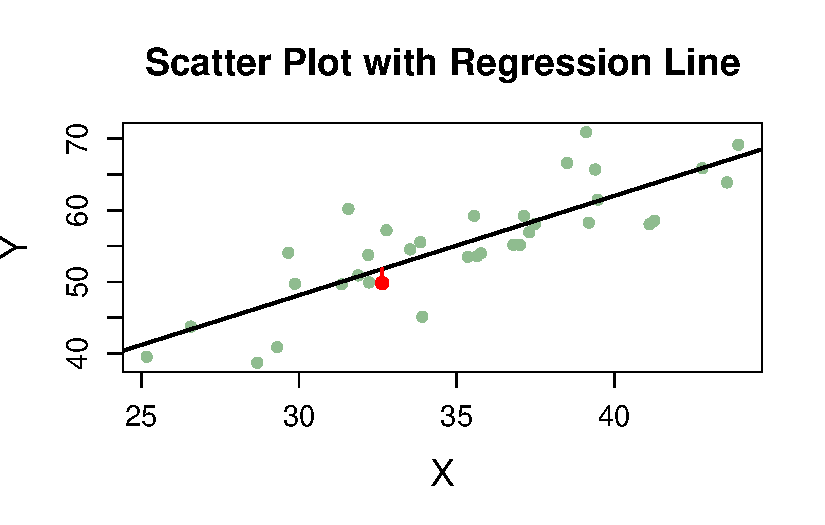
\includegraphics[keepaspectratio]{00_ModelConcepts_files/figure-pdf/unnamed-chunk-2-1.pdf}}

\section*{Notation}\label{notation}
\addcontentsline{toc}{section}{Notation}

\markright{Notation}

When we fit the model to our data, we \textbf{estimate} the unknown
parameters using observed data. We denote these estimates using
\textbf{hat notation} to distinguish them from the true (but unknown)
population parameters:

\[
\hat{\beta}_0, \quad \hat{\beta}_1
\]

Similarly, the \textbf{fitted values} (model-predicted responses) are
denoted as:

\[
\hat{Y}_i = \hat{\beta}_0 + \hat{\beta}_1 X_i.
\]

Thus, after fitting the model, the observed response can be rewritten
as:

\[
Y_i = (\hat{\beta}_0 + \hat{\beta}_1 X_i) + e_i = \hat{Y}_i + e_i
\]

where:

\begin{itemize}
\tightlist
\item
  \(\hat{Y}_i\) is the \textbf{fitted (predicted) value}, and
\item
  \(e_i = Y_i - \hat{Y}_i\) is the \textbf{residual}, representing the
  difference between the observed and predicted values.
\end{itemize}

\bookmarksetup{startatroot}

\chapter*{A brief guideline to hypothesis
testing}\label{a-brief-guideline-to-hypothesis-testing}
\addcontentsline{toc}{chapter}{A brief guideline to hypothesis testing}

\markboth{A brief guideline to hypothesis testing}{A brief guideline to
hypothesis testing}

\begin{quote}
These notes have been adapted from the STA1007 notes (authored by Dr Res
Altwegg and Dr Greg Distiller and some other textbooks.
\end{quote}

Hypothesis testing is a statistical procedure of using sample data to
make inferences about populations. Unlike estimation, where the goal is
to quantify a parameter, hypothesis testing assesses whether an observed
effect is statistically significant. More specifically, a hypothesis
test evaluates two mutually exclusive statements about the population
and determines which statement the data supports.

\subsection*{The General Framework}\label{the-general-framework}
\addcontentsline{toc}{subsection}{The General Framework}

Hypothesis testing follows a structured process:

\begin{enumerate}
\def\labelenumi{\arabic{enumi}.}
\tightlist
\item
  \textbf{State the Hypotheses}: Define the null hypothesis (H₀) and the
  alternative hypothesis (H₁).
\end{enumerate}

The basic idea of hypothesis testing is that we set up a so-called null
hypothesis and then ask how likely our data are if the null hypothesis
were true. If they are unlikely, we conclude that we have found evidence
against the null hypothesis, i.e.~the null hypothesis is probably not
true.

The alternative hypothesis covers all the possibilities not covered by
the null hypothesis. If we conclude that the null hypothesis is probably
not true, that means that the alternative hypothesis is probably true.
These two hypotheses are not equal in how we treat them:

\begin{itemize}
\item
  We start by assuming the null is true and check if the data gives
  enough evidence to reject it.
\item
  If the data strongly contradicts the null, we lean toward the
  alternative hypothesis.
\end{itemize}

But we never prove the alternative hypothesis outright---we only show
that the null is unlikely based on the evidence. You can think of the
null hypothesis as representing a baseline against which the data are
compared, whereas the alternative hypothesis is what we really care
about, worry about or want to demonstrate. This is an important
asymmetry and will need some careful reflection.

Below is an example:

Null Hypothesis (\(H_0\)): ``The average weight of chocolate bars is
100g.''

Alternative Hypothesis (\(H_A\)): ``The average weight of chocolate bars
is less than 100g.''

Lack of evidence against \(H_0\) is not the same as evidence for
\(H_0\). We never say that we have evidence for \(H_0\) or that we
accept \(H_0\) as true.

\begin{enumerate}
\def\labelenumi{\arabic{enumi}.}
\setcounter{enumi}{1}
\tightlist
\item
  \textbf{Choose a Test Statistic}: Select an appropriate statistic to
  measure the observed effect.
\end{enumerate}

A numerical function of the data that quantifies the strength of the
observed effect, whose value determines the result of the test. Examples
include the mean difference, proportion difference, or z-score.

\begin{enumerate}
\def\labelenumi{\arabic{enumi}.}
\setcounter{enumi}{2}
\tightlist
\item
  \textbf{Determine the Null Distribution:} Establish what the test
  statistic would look like if H₀ were true.
\end{enumerate}

We have a test statistic and to say something about how likely this test
statistic (or more extreme is) under the null hypothesis, we need the
null distribution of the test statistic (that is the sampling
distribution of the test statistic as if the null hypothesis were true).
We then compared the observed value of the test statistic to that null
distribution and asked ourselves how unusual it is in light of that
distribution.

\begin{enumerate}
\def\labelenumi{\arabic{enumi}.}
\setcounter{enumi}{3}
\tightlist
\item
  \textbf{Compute the P-value:} Calculate the probability of obtaining a
  test statistic as extreme as the observed one under H₀.
\end{enumerate}

The probability of obtaining a result as extreme as the observed one if
H₀ is true. A small P-value (typically \textless0.05) suggests strong
evidence against (\(H_0\)).

\begin{enumerate}
\def\labelenumi{\arabic{enumi}.}
\setcounter{enumi}{4}
\tightlist
\item
  \textbf{Make a Decision:}
\end{enumerate}

In the approach you have been taught, we compare the P-value to a
predefined significance level (\alpha) and conclude whether to reject
\(H_0\). Here we would like to emphasise that the p-value is a measure
of evidence against \(H_0\) - see below!

\section*{One-Sided vs.~Two-Sided
Tests}\label{one-sided-vs.-two-sided-tests}
\addcontentsline{toc}{section}{One-Sided vs.~Two-Sided Tests}

\markright{One-Sided vs.~Two-Sided Tests}

Two-sided test: Tests for deviations in both directions. Example: ``The
average human body temperature is different from 37°C.''

One-sided test: Tests for deviations in a single direction. Example:
``Students who study more than an hour score higher.''

\section*{Decision Making in Hypothesis
Testing}\label{decision-making-in-hypothesis-testing}
\addcontentsline{toc}{section}{Decision Making in Hypothesis Testing}

\markright{Decision Making in Hypothesis Testing}

A small P-value constitutes evidence against \(H_0\). But how small is
small enough? Sometimes, we want to make a firm decision about whether
we can believe that the observed pattern is real or not. This requires
us to choose a threshold for P. This threshold is called the
significance level and denoted by \(\alpha\). If we obtain a P-value
that is smaller than \(\alpha\), we say that we have obtained a
``statistically significant result'' or that ``\(H_0\) is rejected''. If
our P-value is larger than \(\alpha\), we say that our result is ``not
significant'' or that ``\(H_0\) is not rejected''. In most situations,
researchers choose a significance level of \(\alpha\) = 0.05, which
roughly corresponds to the probability of obtaining five heads in a row
when tossing a fair coin, not a very likely event! Different values for
\(\alpha\) are also sometimes used; the next most common significance
level is \(\alpha\) = 0.01.

Before we go further, we want to emphasize that there is nothing magic
about a specific value of \(\alpha\). This threshold is an arbitrary
choice and should not be taken too seriously. There is not much
difference between a P-value of 0.051 and 0.049. Both constitute about
the same strength of evidence against \(H_0\). Yet, when we apply
\(\alpha\) = 0.05, we would reach opposite conclusions in the two cases.
It is always better to report the exact P-value rather than just state P
\(>\) 0.05 or P \(<\) 0.05 or state that a result is ``not significant''
or ``significant''. And it is particularly important not to imply that a
``non-significant'' result means that there is no effect (that would be
saying \(H_0\) is true when we might in fact have some evidence against
it)!

Alas, dividing results into ``significant'' vs ``not significant'' is
very entrenched in many fields and you will encounter these terms a lot.
And used wisely, this distinction can have its merits. So we'll stick
with it.

\part{Experimental Design}

\chapter{Experiments and experimental
design}\label{experiments-and-experimental-design}

There are two fundamental ways to obtain information in research: by
\emph{observation} or by \emph{experimentation}. In an observational
study the observer watches and records information about the subject of
interest. In an experiment, the experimenter actively manipulates
variables hypothesized to affect the response (insert small example).
Although both are important ways of understanding the world around us,
only through experiments can we \textbf{infer causality}.

That is, by designing and conducting an experiment properly, if we
observe a result such as a change in variable A leads to a change in our
response (say variable B), we can confidently conclude that A
\textbf{caused} this change in B. If we were to merely study variable B
and observe that as variable A changes, B also changes without
conducting an experiment, then we can only say that variable A and B are
associated. We could not easily conclude that any change in B is due to
A. It could be some other factor that is correlated with A or it could
be that B caused the change in A! The key is that a well-designed
experiment controls and holds constant (as best we can) all other
factors that might affect the response, so we can be sure the result is
caused by the variable we manipulated.

Imagine a company wants to determine whether their voluntary employee
training program (the explanatory variable) increases productivity (the
response). They decide to track the productivity of employees who chose
to complete the training and those who did not. They note that, on
average, trained employees are more productive. Can we confidently
conclude that the training program caused increased productivity?

This is an observational study since no variable was actively
manipulated, they merely observed and recorded the productivity of two
groups of employees. So, we cannot conclude that completing the training
program increases productivity - we cannot infer causality. It could be
due to many other factors, either observed or unobserved, such as maybe
employees who choose to do the training program are inherently more
motivated and thus productive. Can you think of any other factors?

If they actively manipulate the explanatory variable, training program,
by randomly assigning employees to complete the training program or not
and control other factors by ensuring the employees are as similar as
possible accross the groups (i.e.~conducted an experiment). Any
differences in productivity between the two groups could then be
ascribed to the training program. If they happen to find that the
employees who were assigned the training program are more productive,
they can confidently say that the program caused increased productivity
(and perhaps make it compulsory for all employees!).

Experimental studies are extremely important in research and in
practice. They are almost the only way in which one can control all
factors to such an extent as to eliminate any other possible explanation
for a change in a response other than the variable actively manipulated.
In this course, we only consider experimental studies and those which
aim to compare the effects of a number of \textbf{treatments}
(comparative experiments).

Here are some other reasons for conducting experiments:

\begin{enumerate}
\def\labelenumi{\arabic{enumi}.}
\item
  They are easy to analyse. A well designed experiment results in
  independent estimates of treatment effects which allow us to easily
  interpret the effects.
\item
  Experiments are frequently used to find optimal levels of variables
  which will maximise (or minimise) the response. Such experiments can
  save enormous amounts of time and money. Imagine trying to find the
  optimal settings for producing electricity from coal without proper
  experimentation. Such a trial and error process would be extremely
  costly, wasteful and time consuming. In a similar vein, what if the
  fictional company in our previous example decided to invest a bunch of
  money in fine-tuning their training program based solely on the
  results of an observational study. In reality though, it turns out
  that adjusting their hiring process to identify more keen candidates
  would have been much more efficient and inexpensive.
\item
  In an experiment we can choose exactly those settings or
  \textbf{treatment levels} we are interested in, e.g.~we can
  investigate the effect of different shift lengths (6, 8 or 9 hours) on
  employee productivity or test specific price points (R100, R150, R200)
  to determine which price maximizes sales or revenue. We can actively
  manipulate the variable(s) to the levels we are interested in.
\end{enumerate}

Experimental studies and their design are fundamental to science,
allowing us to further knowledge and test theories. So lets define them
more rigorously. We'll start by introducing some terminology.

\begin{tcolorbox}[enhanced jigsaw, opacitybacktitle=0.6, colbacktitle=quarto-callout-warning-color!10!white, toprule=.15mm, bottomtitle=1mm, breakable, leftrule=.75mm, rightrule=.15mm, left=2mm, colback=white, coltitle=black, toptitle=1mm, colframe=quarto-callout-warning-color-frame, bottomrule=.15mm, title={Establishing causality through observation is possible, but a bit more
difficult.}, arc=.35mm, titlerule=0mm, opacityback=0]

Experiments are the most reliable way to establish causation because
they involve direct manipulation of variables and control for other
factors that might influence the outcome. By ensuring that differences
in results are due to the specific factor being studied, experiments
help avoid misleading conclusions caused by external influences or
chance associations.

However, in some cases, causation can still be inferred from
observational studies, especially when there is a well-understood
relationship between cause and effect, consistent patterns across
different settings, and no plausible alternative explanations. For
example, the link between smoking and lung cancer was established
through observational data, where researchers accounted for other
possible influences and found strong, consistent evidence that smoking
increases cancer risk. While experiments are preferred, careful analysis
and logical reasoning can sometimes provide enough evidence for causal
claims without direct intervention.

\end{tcolorbox}

\section*{Key points}\label{key-points}
\addcontentsline{toc}{section}{Key points}

\markright{Key points}

\begin{enumerate}
\def\labelenumi{\arabic{enumi}.}
\tightlist
\item
  Two ways of doing research: observation and expermentation.
\item
  Experimentation is the path to causality.
\item
  Experiments actively manipulate variables to isolate their effects on
  a response while controlling everything else.
\item
  We consider comparative experiments where the aim is to compare
  treatments.
\end{enumerate}

\chapter{Terminology}\label{terminology}

\section*{\texorpdfstring{\textbf{Treatment factors, treatment levels
and
treatments:}}{Treatment factors, treatment levels and treatments:}}\label{treatment-factors-treatment-levels-and-treatments}
\addcontentsline{toc}{section}{\textbf{Treatment factors, treatment
levels and treatments:}}

\markright{\textbf{Treatment factors, treatment levels and treatments:}}

The \textbf{treatment factor} is the factor or variable that the
experimenter actively manipulates to measure its effect on the response.
All factors/variables that are investigated, controlled, manipulated,
thought to influence the response, are called the treatment factors.
They become the \textbf{explanatory variables} (mostly categorical) in
the model. For each treatment factor, we actively choose a set of
\textbf{levels}. For example, the treatment factor ``temperature'' can
have levels 10, 20, and 50°C. If temperature is the only treatment
factor in the experiment, the \textbf{treatments}\footnote{The
  terminology of treatments can be traced back to 1920's when it was
  first applied by Ronald Fisher in the agricultural sciences. He is
  often refered to as the Founder of Statistics! Have a look at the very
  first application of ANOVA
  \href{https://www.cambridge.org/core/journals/journal-of-agricultural-science/article/abs/studies-in-crop-variation-i-an-examination-of-the-yield-of-dressed-grain-from-broadbalk/882CB236D1EC608B1A6C74CA96F82CC3}{here}
  and also a \href{https://www.jstor.org/stable/2245989}{nice article}
  describing the history of statistics and his contribution to the
  field.} will also be 10, 20, and 50°C.

If we manipulate more than one factor (e.g., temperature and pressure),
we have two treatment factors. When several treatment factors are
manipulated, the experiment is called factorial and the
\textbf{treatments} are all possible combinations of the factor levels.
If we have pressure levels ``low'' and ``high,'' there are 6 treatments
in total:

\begin{figure}[H]

\centering{

\pandocbounded{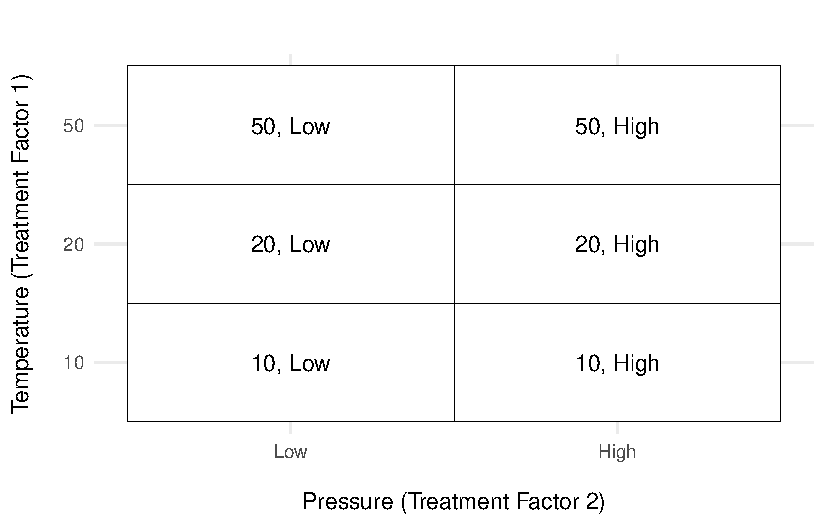
\includegraphics[keepaspectratio]{02_ExpDesign_Term_files/figure-pdf/fig-vistreat-1.pdf}}

}

\caption{\label{fig-vistreat}Visualization of how treatments are formed
as combinations of treatment levels.}

\end{figure}%

In the figure above, there are two treatment factors: Temperature (on
the y-axis) and Pressure (on the x-axis). The axis ticks represent the
levels of each treatment factor, and the blocks within the grid
represent the treatments, which are specific combinations of the levels
of Temperature and Pressure. Each treatment is labeled with the
corresponding combination of levels (e.g., `50, Low' or `10, High').

\begin{tcolorbox}[enhanced jigsaw, opacitybacktitle=0.6, colbacktitle=quarto-callout-warning-color!10!white, toprule=.15mm, bottomtitle=1mm, breakable, leftrule=.75mm, rightrule=.15mm, left=2mm, colback=white, coltitle=black, toptitle=1mm, colframe=quarto-callout-warning-color-frame, bottomrule=.15mm, title={Example 1}, arc=.35mm, titlerule=0mm, opacityback=0]

Three groups of students, 5 in each group, were receiving therapy for
severe test anxiety. Group 1 received 5 hours, group 2 received 10 hours
and group 3 received 15 hours. At the end of therapy each subject
completed an evaluation of test anxiety. Did the amount of therapy have
an effect on the level of test anxiety?

The three groups of students received the scores on the Test Anxiety
index (TAI) at the end of treatment shown in the table below.

\begin{longtable}[]{@{}ccc@{}}
\toprule\noalign{}
Group 1 & Group 2 & Group 3 \\
\midrule\noalign{}
\endhead
\bottomrule\noalign{}
\endlastfoot
48 & 55 & 51 \\
50 & 52 & 52 \\
53 & 53 & 50 \\
52 & 55 & 53 \\
50 & 53 & 50 \\
\end{longtable}

\hfill\break

\end{tcolorbox}

When faced with a text like this, it is useful to identify the treatment
factors, their levels and the treatments, as well the response. Clearly,
from the question, we are interested in the effect of therapy on test
anxiety. A statement like this can generally be read as the effect of
the treatment factor on the response. Nowhere is another treatment
factor mentioned, so we only have one in this example. What are the
levels of therapy we set? The levels are 5, 10 and 15 hours of therapy
and since we only have one factor these are also the treatments. Let's
summarise this as follows:

\begin{itemize}
\tightlist
\item
  \textbf{Response:} Test Anxiety\\
\item
  \textbf{Treatment Factor:} Therapy\\
\item
  \textbf{Treatment Levels:} 5, 10, and 15 hours of therapy\\
\item
  \textbf{Treatments:} 5, 10, and 15
\end{itemize}

\section*{\texorpdfstring{\textbf{Experimental and observational
unit}}{Experimental and observational unit}}\label{experimental-and-observational-unit}
\addcontentsline{toc}{section}{\textbf{Experimental and observational
unit}}

\markright{\textbf{Experimental and observational unit}}

The \textbf{experimental unit} is the entity (e.g.~material, object, or
individual) to which a treatment is assigned or that receives the
treatment. By contrast, the \textbf{observational unit} is the entity
from which the response is recorded. This distinction is very important
because it is the experimental units which determine how often the
treatment has been replicated and therefore the precision with which we
can measure the treatment effect. In the methods that we cover in this
course, we require that in the end there is only one `observation'
(response value) per experimental unit. If several measurements have
been taken on an experimental unit, we will combine these into one
observation, typically by taking the mean. Very often, the experimental
unit is also the observational unit.

What are the experimental units? To determine this, revisit the text of
Example 1 and ask yourself: what entity received the treatments or to
what were treatments applied? Most of you, will probably answer the
students and this is correct. Each student received the respective
treatment (number of hours in therapy) assigned to their group and so
there are \(5 \times 3 = 15\) experimental units.

There is an argument to be made that it is not clear whether the
students received therapy on their own or that the groups of students
received therapy together. In that case, treatments were applied to
groups of students and so there would be three experimental units. This
will usually be clear from the text, but we'll use this scenario to
illustrate some concepts as we go.

We also need to know what the observational units are. The text states
that at the end of therapy, each student completed an evaluation to
determine their level of test anxiety. So the response, test anxiety,
was measured on the student level which means students are the
observational units. In the first scenario, the students are both the
experimental units and observational units. But this would not be the
case if groups are the experimental unit.

We also require that there is only one observation per experimental
unit, the first scenario meets this requirement. For the second
scenario, we have 5 observations per group and so we would have to take
the mean of these values to end up with one response value per group.

Let's add to the summary assuming students are the experimental units:

\begin{itemize}
\tightlist
\item
  \textbf{Experimental unit (no):} Student (15)\\
\item
  \textbf{Observational unit (no):} Student (15)
\end{itemize}

\section*{\texorpdfstring{\textbf{Homogeneity of experimental
units}}{Homogeneity of experimental units}}\label{homogeneity-of-experimental-units}
\addcontentsline{toc}{section}{\textbf{Homogeneity of experimental
units}}

\markright{\textbf{Homogeneity of experimental units}}

When the set of experimental units are as similar as possible such that
there are no distinguishable differences between them, they are said to
be \textbf{homogeneous} (a fancy word for saying they are of the same
kind). The more homogeneous the units are, the smaller the experimental
error variance (natural variation between between observations of the
same treatments) will be. It is super important to have fairly
homogeneous units because it allows us to detect differences between
treatments more easily.

\section*{\texorpdfstring{\textbf{Blocking}}{Blocking}}\label{blocking}
\addcontentsline{toc}{section}{\textbf{Blocking}}

\markright{\textbf{Blocking}}

If the experimental units are not fairly similar but are heterogeneous
(the opposite of homogeneous), we can group them into sets of similar
units. This process is called \textbf{blocking} and the groups are
considered ``blocks''. We compare the treatments within each block as if
each block is its own mini-experiment. This way we account for the
differences between blocks and can better isolate the effect of the
treatments.

\begin{tcolorbox}[enhanced jigsaw, opacitybacktitle=0.6, colbacktitle=quarto-callout-warning-color!10!white, toprule=.15mm, bottomtitle=1mm, breakable, leftrule=.75mm, rightrule=.15mm, left=2mm, colback=white, coltitle=black, toptitle=1mm, colframe=quarto-callout-warning-color-frame, bottomrule=.15mm, title={Example 2}, arc=.35mm, titlerule=0mm, opacityback=0]

Imagine you're testing the effectiveness of two marketing strategies (A
and B) to increase sales at a chain of coffee shops. The coffee shops
are located in different neighborhoods, where factors like income levels
might influence sales. To prevent these differences from skewing the
results, you group the coffee shops into ``blocks'' based on
neighborhood characteristics such as income level (e.g., low, medium,
high).

Within each block, you randomly assign coffee shops to either Strategy A
or Strategy B. This approach allows you to compare the strategies while
controlling for variability caused by differences in neighborhood
features.

Without blocking, would you be able to confidently attribute differences
in sales to the strategies alone? Likely not, as any observed
differences could be due to neighborhood-specific factors rather than
the strategies themselves.

\end{tcolorbox}

\section*{\texorpdfstring{\textbf{Replication and
pseudoreplication}}{Replication and pseudoreplication}}\label{replication-and-pseudoreplication}
\addcontentsline{toc}{section}{\textbf{Replication and
pseudoreplication}}

\markright{\textbf{Replication and pseudoreplication}}

If a treatment is applied independently to more than one experimental
unit it is said to be \textbf{replicated}. Treatments must be
replicated! Making more than one observation on the same experimental
unit is not replication, but \emph{pseudoreplication}. Pseudoreplication
is a common fallacy. The problem is that without true replication, we
don't have an estimate of uncertainty, of how repeatable, or how
variable the result is if the same treatment were to be applied
repeatedly.

In Example 1, if experimental units were the groups and we didn't take
the average of the observations per group, we would have
pseudoreplication as each student would not be an independent replicate
of a treatment - effectively, we have only applied each treatment once.
You might notice that we then only have one true replicate per treatment
group and this is problematic. To get an estimate of uncertainty, we
would have to repeat this experiment a few more times to get more than
one proper replicate.

The first scenario, however, did not have this problem and each
treatment was replicated five times. After going through all this, we
have the following summary:

\begin{itemize}
\tightlist
\item
  \textbf{Response:} Test Anxiety\\
\item
  \textbf{Treatment Factor:} Therapy\\
\item
  \textbf{Treatment Levels:} 5, 10, and 15 hours of therapy\\
\item
  \textbf{Treatments:} 5, 10, and 15\\
\item
  \textbf{Experimental unit (no):} Student (15)\\
\item
  \textbf{Observational unit (no):} Student (15)\\
\item
  \textbf{Replicates:} 5
\end{itemize}

\begin{tcolorbox}[enhanced jigsaw, opacitybacktitle=0.6, colbacktitle=quarto-callout-tip-color!10!white, toprule=.15mm, bottomtitle=1mm, breakable, leftrule=.75mm, rightrule=.15mm, left=2mm, colback=white, coltitle=black, toptitle=1mm, colframe=quarto-callout-tip-color-frame, bottomrule=.15mm, title=\textcolor{quarto-callout-tip-color}{\faLightbulb}\hspace{0.5em}{Tip}, arc=.35mm, titlerule=0mm, opacityback=0]

Creating a summary like this, is a handy exercise for any experiment you
come across, and we'll keep doing it for every experiment in this book.
As we go along, we'll also add information about the type of experiment
that was conducted.

\end{tcolorbox}

\chapter*{The three R's of experimental
design}\label{the-three-rs-of-experimental-design}
\addcontentsline{toc}{chapter}{The three R's of experimental design}

\markboth{The three R's of experimental design}{The three R's of
experimental design}

\textbf{Experimental Design} is a detailed procedure for grouping, if
blocking is necessary, experimental units and for how treatments are
assigned to the experimental units. There are three fundamental
principles, known as the `three R's of experimental design' which are at
the core of a good experiment. The following section might feel a bit
repetitive, but these concepts cannot be emphasised enough.

\section*{Replication}\label{replication}
\addcontentsline{toc}{section}{Replication}

\markright{Replication}

Let's define it again: replication is when each treatment is applied to
several experimental units. This ensures that the variation between two
or more units receiving the same treatment can be estimated and valid
comparisons can be made between treatments. In other words, replication
allows us to separate variation due to differences between treatments
from variation within treatments. For true replication, each treatment
should be \textbf{independently} applied to several experimental units.
If this is not the case, treatment effects become confounded with other
factors.

Confounding means that is not possible to separate the effects of two
(or more) factors on the response, i.e.~it is not possible to say which
of the two factors is responsible for any changes in the response. This
is what happened in the Example 1 when groups are the experimental
units. With only one replicate per treatment, the effect of therapy is
confounded with the experimental unit or the effect of group on test
anxiety. The reason why this is a problem is that any difference between
the treatments could be due to any differences between the groups and
not just the number of therapy hours. The same would be true if we only
had one student per group. Why? Take a moment to think about this.

Consider the first row of the data from Example 1. It looks like the
student in group 2 scored the highest, followed by group 3 and then
group 1. So does longer therapy sessions lead to higher test anxiety?
Likely not! With only one student per treatment, we are not able to say
that any differences in the response are due to the treatments. It could
be due to any differences between the individuals. Maybe the student in
group 3 tends to score higher on anxiety tests regardless of the
treatment, or perhaps the student in group 1 was unusually calm that
day. Without replication, these individual differences could mask (or
mimic) the true effects of the treatments.

By replicating the treatments across multiple students, we can average
out these individual differences and gain a clearer picture of whether
therapy duration truly impacts test anxiety. With five students per
group, we might observe that group 1 consistently scores lower than
group 3. This consistency would provide stronger evidence that the
treatments, and not just individual variation, are responsible for the
observed differences. So by replication, we can compare within treatment
variation to variation between treatments.

\begin{longtable}[]{@{}ccc@{}}
\toprule\noalign{}
Treatment 1 & Treatment 2 & Treatment 3 \\
\midrule\noalign{}
\endhead
\bottomrule\noalign{}
\endlastfoot
48 & 55 & 51 \\
50 & 52 & 52 \\
53 & 53 & 50 \\
52 & 55 & 53 \\
50 & 53 & 50 \\
\end{longtable}

\section*{Randomisation}\label{randomisation}
\addcontentsline{toc}{section}{Randomisation}

\markright{Randomisation}

Randomisation refers to the process of randomly assigning treatments to
experimental units such that each experimental unit has equal chance of
receiving a specific treatment. Randomisation ensures that:

\begin{enumerate}
\def\labelenumi{\arabic{enumi}.}
\item
  There is no bias on the part of the experimenter, either conscious or
  unconscious, when assigning treatments to experimental units.
\item
  No experimental unit is favored to receive a particular treatment.
\item
  Possible differences between units are equally distributed among
  treatments. If there are clear differences between units, then
  blocking should be performed and randomisation occurs within blocks.
  We'll talk more about this when we encounter Randomised Block Designs.
\item
  We can assume independence between observations.
\end{enumerate}

Randomisation is not haphazard. In statistics (and here in the context
of experimental design), randomisation has a specific meaning: namely
that each experimental unit has the same chance of being allocated any
of the treatments. This can be done using random number generators such
as with software packages, dice or drawing number from a hat (provided
the number have been shuffled adequately and have equal chance to be
picked).

Let's have a look at randomisation in R. Suppose we have 4 treatments
(\texttt{A}, \texttt{B}, \texttt{C}, and \texttt{D}) and 32 experimental
units. There are no differences between the units, so we don't have to
block, and we can equally split the units across the treatments, which
means we have 8 units per treatment, i.e., 8 replicates. In R, we first
create a long vector of 8 \texttt{A}s, 8 \texttt{B}s, 8 \texttt{C}s, and
8 \texttt{D}s called \texttt{all.treat}. Then shuffle the vector to
obtain a randomisation using the function \texttt{sample}.

\begin{Shaded}
\begin{Highlighting}[]
\CommentTok{\# repeat the vector A, B, C, D 8 times }
\NormalTok{all.treats }\OtherTok{\textless{}{-}} \FunctionTok{rep}\NormalTok{(}\FunctionTok{c}\NormalTok{(}\StringTok{"A"}\NormalTok{,}\StringTok{"B"}\NormalTok{,}\StringTok{"C"}\NormalTok{,}\StringTok{"D"}\NormalTok{), }\AttributeTok{times =} \DecValTok{8}\NormalTok{)}

\CommentTok{\# permutation of all.treats (sample withut replacement)}
\NormalTok{rand1 }\OtherTok{\textless{}{-}} \FunctionTok{sample}\NormalTok{(all.treats)}

\CommentTok{\# example output}
\NormalTok{rand1}
\end{Highlighting}
\end{Shaded}

\begin{verbatim}
 [1] "C" "D" "A" "B" "B" "C" "A" "B" "A" "D" "C" "C" "A" "D" "D" "C" "C" "B" "D"
[20] "C" "C" "B" "B" "A" "B" "D" "D" "B" "A" "A" "A" "D"
\end{verbatim}

Experimental unit 1 recipes the first treatment that appears as the
first element in the shuffled vector, experimental unit 2 receives the
second and so on.

\section*{Reduction of Unexplained Variation
(Blocking)}\label{reduction-of-unexplained-variation-blocking}
\addcontentsline{toc}{section}{Reduction of Unexplained Variation
(Blocking)}

\markright{Reduction of Unexplained Variation (Blocking)}

Unexplained variation (or experimental error variance or within
treatment variance) is largely due to inherent differences between
experimental units. The larger this unexplained variation, the more
difficult it becomes to detect treatment differences (a treatment
signal). To minimise experimental error variance we can control
extraneous factors (i.e.~keeping all else constant) and by choosing
homogeneous experimental units. Otherwise, we can block experimental
units to reduce the variation.

Blocking variables are nuisance factors that might affect your response
or introduce systematic variation in the response and we are typically,
not interested in these. Often, they are factors that cannot be
randomised, e.g.~biological sex of a person, time of day, location of a
warehouse etc. We control the effect of such variables on the response
by blocking for them so that we can investigate the possible effect of a
variable that we are interested in. Usually, in a complete block
experiment, there are as many experimental units per block as there are
treatments, so that each treatment is applied once in every block.
Treatments are randomized to the experimental units in the blocks. We
can then compare the effects of treatments on similar experimental
units, and we can estimate the variation induced in the response due to
the differences between blocks. This variation due to blocks can then be
removed from the unexplained variation.

Blocking also offers the opportunity to test treatments over a wider
range of conditions, e.g.~if I only use people of one age in my
experiment (say students) I cannot generalize my results to older
people. However, if i use different age blocks I will be able to tell
whether the treatments have similar effects in all age groups or not.

Lastly, if blocking is not feasible, randomization will ensure that at
least treatments and nuisance factors are not confounded.

\begin{quote}
``Block what you can, randomize what you cannot.''

--- Box, Hunter \& Hunter (1978)
\end{quote}

\chapter{Designing an Experiment}\label{designing-an-experiment}

When planning an experiment we need to decide on:

\begin{itemize}
\tightlist
\item
  treatment factors and their levels
\item
  the response
\item
  experimental material / units
\item
  blocking factors
\item
  number of replicates
\end{itemize}

Some of these will be determined by the research question and how
experimental units are assigned to treatments are determined by the
design. The design that will be chosen for a particular experiment
depends on the \textbf{treatment structure} (determined by the research
question) and the \textbf{blocking structure} (determined by the
available experimental units).

Here are two ways the treatments can be structured:

\begin{enumerate}
\def\labelenumi{\arabic{enumi}.}
\tightlist
\item
  \textbf{Single factor}: the treatments are the levels of a single
  treatment factor.
\item
  \textbf{Factorial}: when more than one factor are of interest, then
  the experiment is said to be a factorial experiment. The treatments
  are constructed by crossing the treatment factors like we did in
  Figure~\ref{fig-vistreat} such that the treatments are all possible
  combinations of the treatment levels. For example, if factor A has
  \(a\) levels and factor B has \(b\) levels, there are \(a \times b\)
  treatments. Such an experiment would then be called an \(a \times b\)
  factorial experiment.
\end{enumerate}

The blocking structure is determined the set of experimental units
chosen or available for the experiment.are there any
structures/differences that need to be blocked? Do I want to include
experimental units of different types to make the results more general?
How many experimental units are available in each block? For the
simplest design in this course, the number of experimental units in each
block corresponds to the number of treatments. This is called a complete
block experiment. There are several other blocking structures, such as
incomplete blocks and blocks with missing values, all with specific
analysis which we will not cover here.

In this course, we cover two basic designs: Completely Randomized
Designs (CRD) and Randomized Block Designs (RBD). For both designs, the
treatment structure can be single or factorial. Where they differ is in
terms of the experimental units and how randomization occurs.

\textbf{\emph{Completely Randomized Designs (CRD)}}

When all experimental units are fairly homogeneous, a CRD is used.
Treatments are randomized to all experimental units.

\textbf{\emph{Randomized Block Design}}

This design is used when all experimental units are not homogeneous or
blocking is required to control a nuisance factor. The treatments are
randomized to the units within blocks.

\part{Single Factor Completely Randomised Designs}

\chapter{Introduction}\label{introduction}

Completely Randomized Designs (CRDs) are the simplest experimental
designs. They are used when experimental units are uniform enough and we
expect them to react similar to a given treatment. In other words, we
have no reason to suspect that a group of experimental units might react
differently to the treatments. We also don't expect any effects (besides
possibly a treatment effect) to cause any systematic changes in the
response. So, we don't have to block for differing experimental units or
any nuisance factors.

Remember experimental design is the procedure for how experimental units
are grouped and treatments are applied. We have already said that there
are no blocks in CRDs. So randomisation occurs without restriction and
to all experimental units. More generally, each of the \(a\) treatments
are randomly assigned to \(r\) experimental units, such that each
experimental unit is equally likely to receive any of the treatments.
This means that there are \(N = r \times a\) experimental units in
total. We only consider designs that are \emph{balanced} meaning that
there an equal number of experimental units per treatment, i.e.~a
treatment is applied to \(r\) units. The experiment is then said to have
\(r\) replicates.

The aim when analysing CRDs is to determine whether there is an effect
of the treatment factor. We accomplish this by testing for differences
in the treatment means (mean of response values in each treatment)
through analyses different sources of variation in the response. This
will become clear as we progress.

\section{Example: The effect of social media multitasking on classroom
performance.}\label{example-the-effect-of-social-media-multitasking-on-classroom-performance.}

As a student, I used to believe I could multitask effectively. I would
scroll through my phone during lectures, study while texting friends, or
listen to podcast while driving. It felt like I was paying attention to
everything, but in hindsight, I can barely recall the details of those
podcasts. I often had to revisit lectures or restart study sessions
because my focus wasn't truly there. This tendency extends beyond
student life. In the average workplace, tasks are frequently interrupted
by social media, email checks, or notifications. Many of us feel the
constant pull of our phones when trying to concentrate, whether we're
working, studying, or even relaxing.

In an era of perceived multitasking, where devices and distractions
dominate our attention, it's worth asking: Does social media
multitasking impact academic performance of students?

\begin{tcolorbox}[enhanced jigsaw, opacitybacktitle=0.6, colbacktitle=quarto-callout-warning-color!10!white, toprule=.15mm, bottomtitle=1mm, breakable, leftrule=.75mm, rightrule=.15mm, left=2mm, colback=white, coltitle=black, toptitle=1mm, colframe=quarto-callout-warning-color-frame, bottomrule=.15mm, title={Example 5.1}, arc=.35mm, titlerule=0mm, opacityback=0]

Two researchers from Turkey, Demirbilek and Talan
(\citeproc{ref-multitask2018}{2018}), conducted a study to try and
answer this question. Specifically, they examined the impact of social
media multitasking during live lectures on students' academic
performance.

A total of 120 first-year undergraduate students from the same Turkish
University were randomly assigned to one of three groups:

\begin{enumerate}
\def\labelenumi{\arabic{enumi}.}
\tightlist
\item
  \textbf{Control Group:} Students used traditional pen-and-paper
  note-taking.
\item
  \textbf{Experimental Group 1 (Exp 1):} Students engaged in SMS texting
  during the lecture.
\item
  \textbf{Experimental Group 2 (Exp 2):} Students used Facebook during
  the lecture.
\end{enumerate}

Over a three-week period, participants attended the same lectures on
Microsoft Excel. To measure academic performance, a standardised test
was administered.

\end{tcolorbox}

\textbf{The analysis of experimental data is determined by the design.}
This is the first thing we need to investigate. The design dictates the
terms that we will include in our statistical model and so it is crucial
to be able to identify the design and all factors included (blocking and
treatment). It is also important to check that randomisation has been
done correctly and determine the number of replicates used. In the
previous chapter we started doing this by creating a summary of the
design and we do the same here. From the description of the study, it is
clear that:

\begin{itemize}
\tightlist
\item
  \textbf{Response Variable:} Academic performance, as measured by test
  scores.
\item
  \textbf{Treatment Factor:} Level of social media multitasking.
\item
  \textbf{Treatment Levels (Groups):} Control, Exp 1, and Exp 2.
\end{itemize}

Students were randomly assigned to one of the three groups, and
performance was measured for each individual. Although this may seem
obvious, they only took one measurement per student, so we don't have to
worry about pseudoreplication. This setup indicates that the students
are both the experimental units and the observational units in this
study. With a total of 120 experimental units and three treatments, the
experiment has 40 replicates. Since only one treatment factor was
investigated, and no blocking was performed, this is classified as a
\textbf{single-factor Completely Randomized Design (CRD).} Here is the
study breakdown:

\begin{itemize}
\tightlist
\item
  \textbf{Response Variable:} Academic Performance\\
\item
  \textbf{Treatment Factor:} Level of Social Media Multitasking\\
\item
  \textbf{Treatment Levels:} Control, Experimental 1 (SMS), Experimental
  2 (Facebook)\\
\item
  \textbf{Treatments:} Control, Experiment 1, Experiment 2\\
\item
  \textbf{Experimental Unit:} Student (120)\\
\item
  \textbf{Observational Unit:} Student (120)\\
\item
  \textbf{Replicates:} 40 students per group\\
\item
  \textbf{Design Type:} Single-Factor Completely Randomized Design (CRD)
\end{itemize}

Before we continue, now is the time to note that we won't be using the
real data collected in this experiment. It wasn't available but I have
simulated data to match their results. I've also made some other
modifications such as the original study included 122 students but to
ensure a balanced design I include only 120.

\section{Exploratory data analysis
(EDA)}\label{exploratory-data-analysis-eda}

Before we start any analyses, we have to conduct some exploratory data
analysis to get a feel for our data. We start by checking whether it has
been read in correctly and then look at some descriptive statistics.

In R, we read in the data set and then use some commands to inspect the
data set:

\begin{Shaded}
\begin{Highlighting}[]
\NormalTok{multitask }\OtherTok{\textless{}{-}} \FunctionTok{read.csv}\NormalTok{(}\StringTok{"Datasets/multitask\_performance.csv"}\NormalTok{)}
\FunctionTok{nrow}\NormalTok{(multitask) }\CommentTok{\# check number of rows}
\end{Highlighting}
\end{Shaded}

\begin{verbatim}
[1] 120
\end{verbatim}

\begin{Shaded}
\begin{Highlighting}[]
\FunctionTok{head}\NormalTok{(multitask) }\CommentTok{\# check first 5 rows }
\end{Highlighting}
\end{Shaded}

\begin{verbatim}
    Group Posttest
1    Exp1 86.39427
2    Exp1 64.19996
3    Exp2 52.75394
4 Control 67.81147
5    Exp1 52.39911
6    Exp1 56.58150
\end{verbatim}

\begin{Shaded}
\begin{Highlighting}[]
\FunctionTok{tail}\NormalTok{(multitask) }\CommentTok{\# check last 5 rows }
\end{Highlighting}
\end{Shaded}

\begin{verbatim}
      Group Posttest
115 Control 77.94344
116 Control 63.58444
117    Exp1 55.17758
118    Exp2 67.16150
119    Exp2 32.58373
120    Exp2 49.58119
\end{verbatim}

\begin{Shaded}
\begin{Highlighting}[]
\FunctionTok{summary}\NormalTok{(multitask)}
\end{Highlighting}
\end{Shaded}

\begin{verbatim}
    Group              Posttest    
 Length:120         Min.   :23.38  
 Class :character   1st Qu.:52.67  
 Mode  :character   Median :65.01  
                    Mean   :63.59  
                    3rd Qu.:76.32  
                    Max.   :98.78  
\end{verbatim}

The data set consists of 120 rows (each row representing a student) and
two columns (\texttt{Group} and \texttt{Posttest}). The first column,
\texttt{Groups}, contains the treatment the student was assigned and the
\texttt{Posttest} column contains the response measure. Using the
functions \texttt{head} and \texttt{tail}, we can look at the first and
last 5 rows and the function \texttt{summary} provides us with a
description of each column. We do this to check that R has read in our
data correctly (you can view the whole data set by running
\texttt{view(multitask)} as well). The summary tells us that the
\texttt{Group} column is of the class ``character''. For our analysis,
we want it to be read as a factor:

\begin{Shaded}
\begin{Highlighting}[]
\NormalTok{multitask}\SpecialCharTok{$}\NormalTok{Group }\OtherTok{\textless{}{-}} \FunctionTok{as.factor}\NormalTok{(multitask}\SpecialCharTok{$}\NormalTok{Group)}
\FunctionTok{summary}\NormalTok{(multitask)}
\end{Highlighting}
\end{Shaded}

\begin{verbatim}
     Group       Posttest    
 Control:40   Min.   :23.38  
 Exp1   :40   1st Qu.:52.67  
 Exp2   :40   Median :65.01  
              Mean   :63.59  
              3rd Qu.:76.32  
              Max.   :98.78  
\end{verbatim}

Now, we can see that there are 40 replicates per treatment group,
confirming that the experiment is balanced. I have assumed that, based
on the results shown, that the \texttt{Posttest} scores were recorded as
percentages and using the summary we can quickly check whether there are
any observations that are not on the appropriate scale or might be
outliers. Looks good so far!

\section{Checking assumptions}\label{checking-assumptions}

Demirbilek and Talan (\citeproc{ref-multitask2018}{2018}) had several
research questions, but here we only consider the following:

Are there any differences in mean academic performance between the three
groups?

You might think that we could perform three t-tests (Control vs Exp 1,
Control vs Exp 3, Exp 1 vs Exp 2). We could, but the problem with this
approach is what we call multiple testing. When conducting many tests,
there is an increased risk of making a Type 1 Error (rejecting the null
hypothesis when it is in fact true) \footnote{Can't remember what a
  \(t\)-test is and/or need a refresher on hypothesis testing? Have a
  look this video on t-tests and document for a brief reminder.
  \textbf{Also, a quick (and cool) sidenote:} This study by Chen et al.
  (\citeproc{ref-chen2024effect}{2024}) used a Completely Randomized
  Design (CRD), randomly assigning undergraduate students to playback
  speed groups (1x, 1.5x, 2x, and 2.5x) to measure the effect on
  comprehension of recorded lectures. Using ANOVA they found that
  comprehension was preserved up to 2x speed. I personally like to
  increase the playback speed to 1.5px if I just need to revise
  something quickly.}.

When we have more than two groups, we can use a one-way analysis of
variance (ANOVA) which can be seen as an extension of a \(t\)-test and
is called ``one-way'' because there is a single factor being considered.
In the next section, we will see that ANOVA is a linear model and some
of the assumptions are about the model errors (just like regression):

\begin{enumerate}
\def\labelenumi{\arabic{enumi}.}
\tightlist
\item
  There are no outliers.
\item
  The errors are independent.
\item
  The errors are normally distributed.
\item
  All groups have equal population variances.
\end{enumerate}

We need to check the validity of these assumptions. There are both
formal and informal techniques. Formal techniques (i.e.~hypothesis
tests) are not always appropriate for several reasons such as small data
sets or that testing one assumption usually requires that the other two
hold, complicating the order of tests. Informal techniques are more than
sufficient and in this course, we stick with them.

\subsection*{Outliers}\label{outliers}
\addcontentsline{toc}{subsection}{Outliers}

Outliers are unusual observations (response values) that deviate
substantially from the remaining data points. They can have a large
influence on the estimates of our model. Think of statistics such as
means and variances, outlying observations will shift the mean towards
them and distort the variability of the data.

If we're lucky, outliers are artefacts of data recording or entering
issues, such as a missing decimal points or incorrect scaling (called
error outliers). These types of outliers can be corrected and the
analysis can be done as usual. If, however, there are freak observations
that are not clearly due to anything like data inputting, then they are
likely genuine unusual responses (called interesting outliers) and
should not be discarded. There are many ways of identifying and dealing
with outliers (Aguinis, Gottfredson, and Joo
(\citeproc{ref-outlier1}{2013}) found 29 different ways in the
literature). Here, it is recommended that the analysis should be run
with and without the outliers to see whether the conclusion depends on
their inclusion. When dealing with outliers, it is best to be
transparent and clear about how they were handled. Simply removing
outliers with no explanation is questionable research practice.

A good way to check for outliers, is to inspect the data visually with a
box-plot of your data grouped by treatment.

\begin{Shaded}
\begin{Highlighting}[]
\FunctionTok{boxplot}\NormalTok{(Posttest }\SpecialCharTok{\textasciitilde{}}\NormalTok{ Group, }\AttributeTok{data =}\NormalTok{ multitask, }\AttributeTok{col =} \FunctionTok{c}\NormalTok{(}\StringTok{"skyblue"}\NormalTok{, }\StringTok{"lightgreen"}\NormalTok{, }\StringTok{"pink"}\NormalTok{), }
        \AttributeTok{main =} \StringTok{"Posttest Scores by Group"}\NormalTok{, }
        \AttributeTok{xlab =} \StringTok{"Group"}\NormalTok{, }
        \AttributeTok{ylab =} \StringTok{"Posttest Scores"}\NormalTok{)}

\FunctionTok{stripchart}\NormalTok{(Posttest}\SpecialCharTok{\textasciitilde{}}\NormalTok{Group, }\AttributeTok{data =}\NormalTok{ multitask, }\AttributeTok{vertical =} \ConstantTok{TRUE}\NormalTok{, }\AttributeTok{add =} \ConstantTok{TRUE}\NormalTok{, }\AttributeTok{method =} \StringTok{"jitter"}\NormalTok{)}
\end{Highlighting}
\end{Shaded}

\begin{figure}[H]

\centering{

\pandocbounded{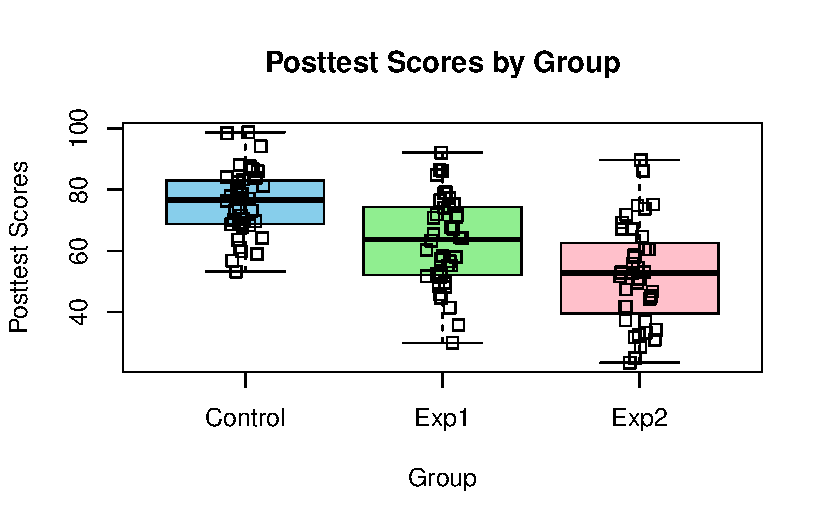
\includegraphics[keepaspectratio]{05_CRD_Intro_files/figure-pdf/fig-socialbox-plot-1.pdf}}

}

\caption{\label{fig-socialbox-plot}Box-plots of Post treatment scores by
group.}

\end{figure}%

The first line of code plots the box-plot and by inputting
\texttt{Posttest\textasciitilde{}Groups} as the first argument we are
say plot the values of \texttt{Posttest} by \texttt{Groups}. There are
extra graphical parameters specified to make the plot look a bit nicer.
The function \texttt{stripchart} is used to overlay the data points.
Based on these plots, there aren't any obvious outlying observations.

\subsection*{Equal population variance}\label{equal-population-variance}
\addcontentsline{toc}{subsection}{Equal population variance}

The model assumes that population variances in different levels of the
treatment factor are equal. That is, it is assumed in ANOVA that the
variance of the response within each treatment is a separate estimate of
the same population variance.

Since we only have sample data, we would not expect that the sample
variances to be exactly the same. If they are different it does not mean
the assumption is not met. We expect them to differ a bit due to chance
simply because we are sampling. Every time we sample from a population,
the data set will be different and so will it's variability. The sample
variances need to be similar enough so that our assumption of equal
population variance is reasonable.

To check this assumption, we can inspect the box-plots again and compare
the heights. More specifically, we look at the interquartile ranges
(IQR). From looking at the plot, the IQRs do not vary widely. If you
prefer to look at the actual values, we can use R to obtain them:

\begin{Shaded}
\begin{Highlighting}[]
\FunctionTok{sort}\NormalTok{(}\FunctionTok{tapply}\NormalTok{(multitask}\SpecialCharTok{$}\NormalTok{Posttest,multitask}\SpecialCharTok{$}\NormalTok{Group,IQR))}
\end{Highlighting}
\end{Shaded}

\begin{verbatim}
 Control     Exp2     Exp1 
14.01068 20.94529 21.97001 
\end{verbatim}

Another measure of variability we can look at, are the standard
deviations (sd's). With the same line of code but just replacing the
function we want to apply, we obtain the sd of each group:

\begin{Shaded}
\begin{Highlighting}[]
\FunctionTok{sort}\NormalTok{(}\FunctionTok{tapply}\NormalTok{(multitask}\SpecialCharTok{$}\NormalTok{Posttest,multitask}\SpecialCharTok{$}\NormalTok{Group,sd))}
\end{Highlighting}
\end{Shaded}

\begin{verbatim}
 Control     Exp1     Exp2 
10.82887 14.60601 16.42678 
\end{verbatim}

The rule of thumb is to use the ratio of the smallest to largest
standard deviation and check whether it is smaller than five. In our
case, the smallest sd (of the Control group) is about 1.5 times smaller
than the largest sd (of the Exp 2 group) which is acceptable.

\subsection*{Normally distributed
errors}\label{normally-distributed-errors}
\addcontentsline{toc}{subsection}{Normally distributed errors}

We can check this assumption by looking at the residuals after model
fitting. A common misconception is to think that the response needs to
be normally distributed. However, it is only the unexplained variation,
i.e.~the errors or residuals (estimates of errors), that we assume to be
normally distributed. Of course, if the response has a clearly
non-normal distribution (e.g.~Binomial), then the residuals are likely
to be non-normal as well. So, we can check our response values before
hand for obvious deviation from normality, but we have to check this
assumption again after fitting our model. Things to look for are
asymmetric box-plots which indicate skew distributions. We also want to
check that the data points tend to cluster around the median. In
Figure~\ref{fig-socialbox-plot}, there are no signs of any clear
deviation from normality. Other graphs we could look at are histograms
or Quantile-Quantile (Q-Q) plots. Q-Q plots show the theoretical
quantiles of the standard normal distribution against the actual
quantiles of our data. We want our data to be as close to the xy line as
possible (deviations in the tails are expected).

\begin{Shaded}
\begin{Highlighting}[]
\FunctionTok{par}\NormalTok{(}\AttributeTok{mfrow =} \FunctionTok{c}\NormalTok{(}\DecValTok{1}\NormalTok{,}\DecValTok{3}\NormalTok{))}

\CommentTok{\# First we subset the data for each group}
\NormalTok{control }\OtherTok{\textless{}{-}}\NormalTok{ multitask}\SpecialCharTok{$}\NormalTok{Posttest[multitask}\SpecialCharTok{$}\NormalTok{Group }\SpecialCharTok{==} \StringTok{"Control"}\NormalTok{]}
\NormalTok{exp1 }\OtherTok{\textless{}{-}}\NormalTok{ multitask}\SpecialCharTok{$}\NormalTok{Posttest[multitask}\SpecialCharTok{$}\NormalTok{Group }\SpecialCharTok{==} \StringTok{"Exp1"}\NormalTok{]}
\NormalTok{exp2 }\OtherTok{\textless{}{-}}\NormalTok{ multitask}\SpecialCharTok{$}\NormalTok{Posttest[multitask}\SpecialCharTok{$}\NormalTok{Group }\SpecialCharTok{==} \StringTok{"Exp2"}\NormalTok{]}


\FunctionTok{qqnorm}\NormalTok{(control, }\AttributeTok{pty =} \DecValTok{4}\NormalTok{, }\AttributeTok{col =}\StringTok{"blue"}\NormalTok{, }\AttributeTok{main =} \StringTok{"Control"}\NormalTok{)}
\FunctionTok{qqline}\NormalTok{(control, }\AttributeTok{col =} \StringTok{"red"}\NormalTok{)}

\FunctionTok{qqnorm}\NormalTok{(exp1, }\AttributeTok{pty =} \DecValTok{4}\NormalTok{, }\AttributeTok{col =}\StringTok{"blue"}\NormalTok{, }\AttributeTok{main =} \StringTok{"Exp 1"}\NormalTok{)}
\FunctionTok{qqline}\NormalTok{(exp1, }\AttributeTok{col =} \StringTok{"red"}\NormalTok{)}

\FunctionTok{qqnorm}\NormalTok{(exp2, }\AttributeTok{pty =} \DecValTok{4}\NormalTok{, }\AttributeTok{col =}\StringTok{"blue"}\NormalTok{, }\AttributeTok{main =} \StringTok{"Exp 2"}\NormalTok{)}
\FunctionTok{qqline}\NormalTok{(exp2, }\AttributeTok{col =} \StringTok{"red"}\NormalTok{)}
\end{Highlighting}
\end{Shaded}

\begin{figure}[H]

\centering{

\pandocbounded{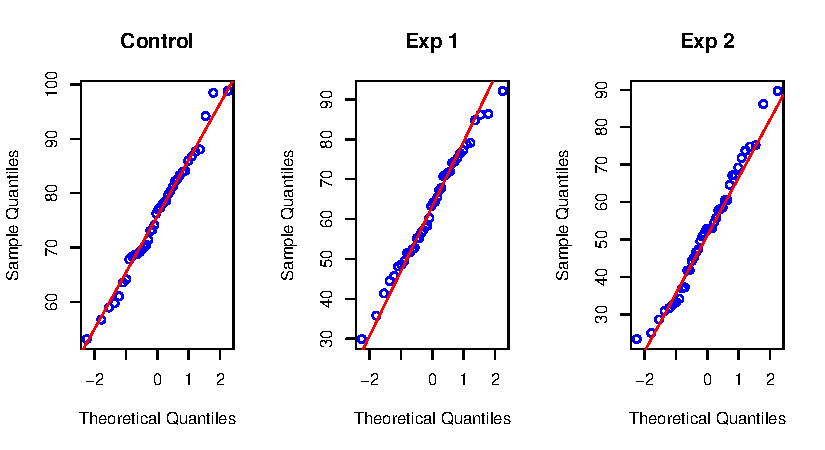
\includegraphics[keepaspectratio]{05_CRD_Intro_files/figure-pdf/fig-socialqq-1.pdf}}

}

\caption{\label{fig-socialqq}Q-Q plots of response per treatment group.}

\end{figure}%

The \texttt{qqnorm} function plots the theoretical quantiles on the
x-axis and the sample quantile son the y-axis. So each point on the plot
corresponds to a quantile from the sample plotted against the expected
quantile from the standard normal distribution. As a reference we add a
straight 45-degree line (in red) using the \texttt{qqline} function to
indicate what perfect normality would look like.

\subsection*{Independent errors}\label{independent-errors}
\addcontentsline{toc}{subsection}{Independent errors}

The assumption is that the \textbf{errors} are independent. While we can
check for certain types of dependence in the residuals after fitting the
ANOVA (as we will see later), dependence among observations generally
results in dependent residuals. Therefore, before fitting any models, we
examine the observations and the experimental design to identify
potential violations of independence.

In statistics, if one observation influences another in some way or
another, they are said to be dependent. For the type of data considered
here, there are two types of independence we require. Firstly,
observations within treatments should be independent and second,
observations between samples should be independent. Another way of
saying this, is \textbf{there should be independence within and among
treatments.} Depending on the direction of any violations, the within
treatment variance or among treatment variance can either be deflated or
inflated and treatment effects can be biased. This has considerable
impact on the test statistic (F-ratio for ANOVA, more on this later)
which could lead to misleading results. \footnote{Underwood
  (\citeproc{ref-underwood_1996}{1996}) has a very detailed explanation
  of the independence assumption (and the others) in the context of
  ANOVA. The book is for ecological experiments, but much of it pertains
  to all types of experiments.}

Violations of independence typically occur when the experimental units
within or among treatments are connected in some way. Dependence within
a sample can occurs when they are taken in a non-random sequence. Doing
so typically allows some other variable to introduce dependence between
successive observations. For example, measurement drift (when a tool's
reading gradually changes over time), physical effects
(e.g.~temperature) of the location of experimental units or the
experimenter might become better (or worse) at taking the measurement as
they move along. If these variables are not taken into account (by
including them as factors in the model), it leads to a lack of
independence in the errors of our model. Specifically, they lead to
auto-correlated residuals; observations made closer together in time or
space are more similar to each other than expected (this is what we
check after model fitting).

An informal check we could do, is to plot the data in the order in which
they were collected (if this information is available) whether that is
temporally or spatially to see if any patterns emerge. To do this in R,
we can create a Cleveland dot plot.

\begin{Shaded}
\begin{Highlighting}[]
\FunctionTok{dotchart}\NormalTok{(multitask}\SpecialCharTok{$}\NormalTok{Posttest, }\AttributeTok{ylab =} \StringTok{"Order of observation"}\NormalTok{, }\AttributeTok{xlab =}\StringTok{"Post treatment test score"}\NormalTok{)}
\end{Highlighting}
\end{Shaded}

\begin{figure}[H]

\centering{

\pandocbounded{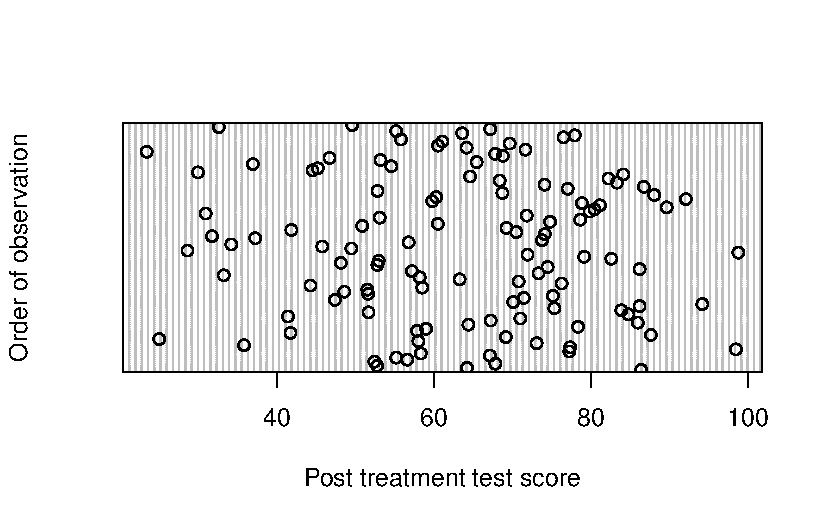
\includegraphics[keepaspectratio]{05_CRD_Intro_files/figure-pdf/fig-socialdotchart-1.pdf}}

}

\caption{\label{fig-socialdotchart}Cleveland dot chart of response
values in the order in which they appear in the data set.}

\end{figure}%

We have assumed that the order in which the observations appear in the
data set are the order in which they were recorded. If there were any
factors that caused systematic trends, (i.e.~dependence) in the
observations, then there would be some kind of pattern in the dot chart.
For our example, there is no clear pattern. After fitting the model, we
can also plot the residuals against spatial coordinate or against order
to check for obvious patterns. This method, however, only detects
violations of independence if observations are related to time or space.

Dependence between treatments can occur if we apply the treatments to
the same group of experimental units or if experimental units from
different treatments are able to interact in some way during the
experiment. These types of violations including those mentioned above,
are ones that we can mostly prevent or control by properly designing the
experiment. When we control for factors that might induce dependence, we
can include them in our model.

Other reasons for dependence may not be as obvious or easy to eliminate
as we will see below. In the end, they may not have a strong impact on
our estimates but it is important to carefully scrutinize your design
and the system you are studying to identify possible sources of
dependence so that these can be addressed and dealt with properly.

In our example, within and among group dependence could be caused by the
students interacting or influencing each other in some way (by sharing
notes for example). During the lectures, this can be controlled by
careful monitoring and randomising their position in the lecture
theater, but outside of lectures, it is less easy to control. Here we
can argue that if students interacted outside of lectures the impact on
their academic performance (as measured by the test) would likely be
negligible. The integrity of the students is at play. It is not really
possible to diagnose this type of dependence after the fact, only with
careful design and implementation can these be avoided.

\textbf{It is the onus of the experimenter to design and conduct
experiments that ensure independence.} With more thought (and if we're
lucky, funding) all well-designed experiments should lead to independent
data. If violations are found after the fact, they cannot typically be
corrected and then methods that deal specifically with dependent data
(if appropriate) should be used\footnote{A few of these methods are
  repeated measures ANOVA, mixed-models or hierarchical models.}.

\subsection*{A quick note on the robustness of
ANOVA}\label{a-quick-note-on-the-robustness-of-anova}
\addcontentsline{toc}{subsection}{A quick note on the robustness of
ANOVA}

A statistical procedure is said to be robust to departures from a model
assumption if the results remain unbiased even when the assumption is
not met. The robustness of ANOVA is as follows:

\begin{enumerate}
\def\labelenumi{\arabic{enumi}.}
\item
  The assumption of normality is not super crucial. Only severe
  departures from normality such as long-tailed distributions or skewed
  distributions when sample sizes are unequal and/or small are
  particularly problematic.
\item
  Independence within and among groups is extremely important. ANOVA
  does not handle dependent data and other analyses should be attempted
  if there is dependence.
\item
  ANOVA is relatively robust to violations of the equal variance
  assumption as long as there are no outliers, sample sizes are large
  and fairly equal (in the case of unbalanced designs which we do not
  cover here), and the sample variances are relatively equal.
\item
  ANOVA is not very resistant to severely outlying observations either.
\end{enumerate}

\begin{tcolorbox}[enhanced jigsaw, opacitybacktitle=0.6, colbacktitle=quarto-callout-tip-color!10!white, toprule=.15mm, bottomtitle=1mm, breakable, leftrule=.75mm, rightrule=.15mm, left=2mm, colback=white, coltitle=black, toptitle=1mm, colframe=quarto-callout-tip-color-frame, bottomrule=.15mm, title=\textcolor{quarto-callout-tip-color}{\faLightbulb}\hspace{0.5em}{Note}, arc=.35mm, titlerule=0mm, opacityback=0]

\begin{enumerate}
\def\labelenumi{\arabic{enumi}.}
\item
  In this course, you will always encounter data that has already been
  collected and the description of the experiment will likely not be
  very exhaustive. You might be task then with thinking about how the
  assumption of independence could have been violated, but for the most
  part we will assume the data are independent, both within and among
  samples (unless otherwise stated or you are asked if the assumption
  holds).
\item
  No real data set ever meets all assumptions of a model perfectly. As
  the famous (at least in the world of statistics) quote by George Box
  goes: ``All models are wrong but some are useful.'' Judging whether a
  particular data set meets our assumptions reasonably well is therefore
  a bit of an art. You will likely read and hear that being able to
  identify violations comes from \textbf{experience}. The best way to
  get experience is to look at lots of data sets where you know how well
  they meet the assumptions. That's best done via simulation. We
  therefore encourage you to use the attached R code to simulate data
  where various assumptions are violated. Run the code a number of times
  to get a feeling for how variable your actual sample can be even if
  the data generating mechanism doesn't change. You may also want to
  play around with the sample sizes and you can change the degree to
  which the assumptions are violated to get a feeling for how these
  violations show up in the plots.
\end{enumerate}

\end{tcolorbox}

\section{Summary}\label{summary}

Completely Randomized Designs (\textbf{CRDs}) are the simplest
experimental designs, used when experimental units are \textbf{uniform}
and expected to react similarly to treatments. Since no nuisance factors
are controlled, randomization occurs \textbf{without restriction}, and
treatments are \textbf{evenly assigned} across experimental units
(\textbf{balanced design}).

The social media multitasking study served as an example, where 120
students were randomly assigned to three groups (Control, SMS, Facebook)
to measure their academic performance. This setup represents a
single-factor CRD, where students are both the experimental and
observational units with 40 replicates per group.

Before conducting ANOVA, we:

\begin{itemize}
\tightlist
\item
  Checked the data set for correct structure (120 observations,
  treatment groups as factors).
\item
  Inspected summary statistics and visualized distributions (box-plots,
  histograms, Q-Q plots).
\end{itemize}

For ANOVA, the following assumptions were examined:

\begin{enumerate}
\def\labelenumi{\arabic{enumi}.}
\tightlist
\item
  \textbf{Outliers}: Check via box-plots.
\item
  \textbf{Equal variance}: Assess using interquartile ranges and ratio
  of sample standard deviations.
\item
  \textbf{Normality of errors}: Verified using Q-Q plots.
\item
  \textbf{Independence within and between treatment groups}: Considered
  through study design.
\end{enumerate}

Proper experimental design ensures valid conclusions. Identifying
violations of assumptions early helps prevent biased results.

\chapter{A Simple Model for a CRD}\label{a-simple-model-for-a-crd}

To analyse data collected from a Completely Randomised Design we could
use \(t\)-tests and compare the samples two at a time. This approach is
problematic for two reasons. Firstly, the test statistic of a \(t\)-test
is calculated with a standard deviation based only on the two samples it
considers. We want our test statistic to consider the variability in all
samples collected. Second, when we conduct multiple tests the overall
Type 1 Error rate increases. That is, when doing many tests, the chance
of making \emph{at least one wrong conclusion} increases with the number
of tests (if you want to know more see the box below). To avoid this, we
will use the ANOVA method which was specifically developed for comparing
multiple means.

\begin{tcolorbox}[enhanced jigsaw, opacitybacktitle=0.6, colbacktitle=quarto-callout-caution-color!10!white, toprule=.15mm, bottomtitle=1mm, breakable, leftrule=.75mm, rightrule=.15mm, left=2mm, colback=white, coltitle=black, toptitle=1mm, colframe=quarto-callout-caution-color-frame, bottomrule=.15mm, title={Multiple Testing / Comparisons}, arc=.35mm, titlerule=0mm, opacityback=0]

When we conduct a test, there is always a possibility that a significant
result is due to chance and not actually a real difference. In first
year, you were taught the Neyman-Pearson approach to hypothesis testing,
which entails setting a significance level (\(\alpha\)) for the test you
will conduct. This significance level is the Type 1 error rate
(probability of falsely rejecting \(H_0\)). A common \(\alpha\) is 0.05,
meaning that 5\% of the time we will reject the null hypothesis even if
it is true. That means when we find a significant result, one of two
things have happened:

\begin{enumerate}
\def\labelenumi{\arabic{enumi}.}
\tightlist
\item
  Either we genuinely found a significant result or,
\item
  We were that unlucky, that our result is one of those 5\% cases.
\end{enumerate}

We will never know, this is the basis of statistical testing. We accept
that we cannot tell which of our conclusions are Type 1 Errors. When we
conduct many tests, the overall Type 1 Error rate increases. That is the
overall chance of \emph{at least one wrong conclusion} increases with
the number of tests conducted. This is not good! We already might be
wrong 5\% and we don't want to increase that risk even further when
conducting multiple tests.

\end{tcolorbox}

\section{The model}\label{the-model}

When we collect samples, we usually want to learn something about the
populations from which they were drawn. To do this, we can develop a
model for the observations that reflects the different sources of
variation believed to be at play.

For Completely Randomised Designs, we have \(a\) treatments which
implies \(a\) population means \(\mu_1, \mu_2, \mu_3, \ldots, \mu_a\).
We are interested in modelling the means of the treatments and the
differences between them. Ultimately we want to test whether they are
equal which we'll get to in the next section. First, we construct a
simple model for each observation \(Y_{ij}\):

\[
Y_{ij} = \mu_{i} + e_{ij},
\]

where

\[
\begin{aligned}
i & = 1, \dots, a \quad (a = \text{number of treatments}) \\
j & = 1, \dots, r \quad (r = \text{number of replicates}) \\
Y_{ij} & = \text{observation of the } j^{th} \text{ unit receiving treatment } i \\
\mu_i & = \text{mean of treatment } i \\
e_{ij} & = \text{random error with } e_{ij} \sim N(0, \sigma^2)
\end{aligned}
\]

That is, each observation is modeled as the sum of its population mean
and some random variation, \(e_{ij}\). This random variation represents
unexplained differences between individual observations within the same
group and we assume that these differences follow a normal distribution
with mean 0 and constant variance across all treatment groups.
\footnote{As opposed to non-constant variance across all treatment
  groups: \(e_{ij} \sim N(0, \sigma^2_{i})\) where the \(\sigma_i^2\)'s
  are different.}

We can change the notation slightly by arbitrarily dividing each mean
into a sum of two components: the overall mean \(\mu\) (the mean of the
entire data set, which is the same as the mean of the \(a\)
means\footnote{\(\mu = \frac{\sum\mu_i}{a}\)}) and the difference
between the population mean and the overall mean. In symbols, this
translates to:

\[
\begin{aligned}
\mu_1 &= \mu + (\mu_1 - \mu) \\
\mu_2 &= \mu + (\mu_2 - \mu) \\
&\;\;\vdots \notag \\
\mu_a &= \mu + (\mu_a - \mu)
\end{aligned}
\]

The difference \((\mu_i - \mu)\) is the \textbf{effect of treatment}
\(i\), denoted by \(A_i\). So each population mean is the sum of the
overall mean and the part that we attribute to the particular treatment
(\(A_i\)):

\[
\mu_i = \mu + A_i, \quad i = 1, 2, \dots, a,
\]

where \(\sum A_i = 0\).

\begin{tcolorbox}[enhanced jigsaw, opacitybacktitle=0.6, colbacktitle=quarto-callout-caution-color!10!white, toprule=.15mm, bottomtitle=1mm, breakable, leftrule=.75mm, rightrule=.15mm, left=2mm, colback=white, coltitle=black, toptitle=1mm, colframe=quarto-callout-caution-color-frame, bottomrule=.15mm, title={Why the \(\sum A_i = 0\) constraint?}, arc=.35mm, titlerule=0mm, opacityback=0]

This constraint ensures that the treatment effects are expressed as
deviations from the overall mean. To see why this holds, take the sum of
both sides of the equation:

\[
\sum_{i=1}^{a} \mu_i = \sum_{i=1}^{a} (\mu + A_i).
\]

Expanding the right-hand side:

\[
\sum_{i=1}^{a} \mu_i = a\mu + \sum_{i=1}^{a} A_i.
\]

By definition, the overall mean \(\mu\) is the mean of the treatment
means:

\[
\mu = \frac{1}{a} \sum_{i=1}^{a} \mu_i.
\]

Multiplying both sides by \(a\) gives:

\[
\sum_{i=1}^{a} \mu_i = a\mu.
\]

Comparing this with our earlier equation:

\[
a\mu = a\mu + \sum_{i=1}^{a} A_i.
\]

Subtracting \(a\mu\) from both sides, we get:

\[
\sum_{i=1}^{a} A_i = 0.
\]

This constraint is standard in ANOVA models to ensure that the treatment
effects are relative to the overall mean rather than being arbitrarily
defined. It is not an additional assumption; any \(a\) means can be
written in this way.

\end{tcolorbox}

Replacing \(\mu_i\) in the model above leads to the common
parameterisation of a single-factor ANOVA model\footnote{Often called
  \textbf{Model I}.}:

\[
Y_{ij} = \mu + A_{i} + e_{ij}
\]

where

\[
\begin{aligned}
i & = 1, \dots, a \quad (a = \text{number of treatments}) \\
j & = 1, \dots, r \quad (r = \text{number of replicates}) \\
Y_{ij} & = \text{observation of the } j^{th} \text{ unit receiving treatment } i \\
\mu & = \text{overall or general mean} \\
A_i & = \text{effect of the } i^{th} \text{ level of treatment factor A} \\
e_{ij} & = \text{random error with } e_{ij} \sim N(0, \sigma^2)
\end{aligned}
\]

\begin{tcolorbox}[enhanced jigsaw, opacitybacktitle=0.6, colbacktitle=quarto-callout-caution-color!10!white, toprule=.15mm, bottomtitle=1mm, breakable, leftrule=.75mm, rightrule=.15mm, left=2mm, colback=white, coltitle=black, toptitle=1mm, colframe=quarto-callout-caution-color-frame, bottomrule=.15mm, title={Comparison to regression}, arc=.35mm, titlerule=0mm, opacityback=0]

If you wanted to, you could rewrite this with the regression notation
you've encountered before as a regression model with a single
categorical explanatory variable:

\[ Y_i = \beta_0 + \beta_1 T2_i + \beta_2 T3_i + e_i \]

where \(T2\) and \(T3\) are indicator variables (i.e.~\(T2 = 1\) if
observation \(i\) is from treatment 2 and 0 otherwise). The intercept
estimates the mean of the baseline category, here it is \(T1\).

These two models are equivalent. The data are exactly the same: in both
situations we have \(a\) groups and we are interested in the mean
response of these groups and the difference between them. The model
notation is just slightly different. In the ANOVA model we use \(\mu\)
and \(A_i\) instead of \(\beta_0\) and \(\beta_i\) which have different
meanings.

\begin{longtable}[]{@{}
  >{\centering\arraybackslash}p{(\linewidth - 2\tabcolsep) * \real{0.5000}}
  >{\centering\arraybackslash}p{(\linewidth - 2\tabcolsep) * \real{0.5000}}@{}}
\toprule\noalign{}
\begin{minipage}[b]{\linewidth}\centering
Regression
\end{minipage} & \begin{minipage}[b]{\linewidth}\centering
ANOVA
\end{minipage} \\
\midrule\noalign{}
\endhead
\bottomrule\noalign{}
\endlastfoot
\(\beta_0\) is the mean of the baseline category & \(\mu\) is the
overall mean \\
\(\beta_1\) is the difference between the means of category 2 and the
baseline category. & \(A_i\) is the effect of treatment \(i\),
i.e.~change in mean response relative to the overall mean. \\
\end{longtable}

When all the explanatory variables are categorical, which is mostly the
case in comparative experimental data, it is more convenient to write
the model in the ANOVA form, for two reasons:

\begin{enumerate}
\def\labelenumi{\arabic{enumi}.}
\item
  The \(A_i\) notation is more concise, because we don't have to add all
  the dummy variables. This makes it easier to read and understand
  because there is only one term per factor.
\item
  Mathematically it is more convenient. In this format all terms are
  deviations from a mean. This leads directly to sums of
  squares\footnotemark{} (squared deviations from a mean) and analysis
  of variance. We will see later that we can partition the total sum of
  squares into one part for every factor in the model. This allows us to
  investigate the variability in the response contributed by every model
  term (or factor).
\end{enumerate}

\end{tcolorbox}

\footnotetext{In statistics, sums of squares is a measure of variability
and refers to squared deviations from a mean or expected value. For
example, the residual sums of squares (sum of squared deviations of the
observations from the fitted values).}

The model can be interpreted as follows:

Each observation, \(Y_{ij}\), is the sum of the overall mean (\(\mu\)),
plus the effect of the treatment it belongs to (\(A_i\)), and some
random error (\(e_{ij}\)). We use two subscripts on the \(Y\). One to
identify the group (treatment) and the other to identify the subject
(experimental unit) within the group:

\[
\begin{aligned}
Y_{1j} &= \mu + A_1 + e_{1j} \\ 
Y_{2j} &= \mu + A_2 + e_{2j} \\ 
Y_{3j} &= \mu + A_3 + e_{3j} \\
&\;\;\vdots \notag \\
Y_{aj} &= \mu + A_a + e_{aj} \\
\end{aligned}
\]

\section{Estimation}\label{estimation}

Okay, so we have a model which we now need to \textbf{fit to our data}.
When we do this, we estimate the model parameters using our data. The
parameters we want to estimate are \(\mu\) (the overall mean), the
treatment effects (\(A_i\)) and \(\sigma^2\) (the error variance). As
for regression, we find \textbf{least squares estimates} for the
parameters which minimise the residual or error sum of
squares\footnote{error = observed - fitted.}:

\[ \text{SSE} = \sum_i\sum_j e_{ij}^2 = \sum_i\sum_j (Y_{ij} - \hat{Y}_{ij})^2 = \sum_i\sum_j (Y_{ij} - \mu - A_i)^2\]

It turns out when we solve for the estimates that minimise the
SSE\footnote{Another name for this is the residual sums of squares
  (RSS).}, we obtain the following estimators:

\[
\begin{aligned}
\hat{\mu} = \bar{Y}_{..} \\
\hat{\mu}_i = \bar{Y}_{i.}
\end{aligned}
\]

and

\[\hat{A}_i =  \bar{Y}_{i.} - \bar{Y}_{..}\]

From linear model theory we know that the above are unbiased
estimates\footnote{Unbiased means that the expected value of these
  statistics equals the parameter being estimated. In other words, the
  statistic equals the true parameter on average.} of \(\mu\) and the
\(A_i\)'s. What does this tell you? It tells you that we can use the
sample means as estimates for the true means. The estimated mean
response for treatment \(i\) is the observed sample mean of treatment
\(i\) and the observed overall mean is the estimated grand mean.

For the last parameter, the error variance, an unbiased estimator is
found by dividing the minimised SSE (i.e.~calculated with the least
squares estimates) by its degrees of freedom:

\[ s^2 = \frac{1}{N-a}\sum_{ij}(Y_{ij} - \bar{Y}_{i.})^2 \]

This quantity is called the Mean Squares for Error (MSE) or residual
mean square. It has \((N-a)\) degrees of freedom since we have \(N\)
observations and have estimated \(a\) means. If you look at the formula
you'll notice that it is an average of the observed variability from the
different treatment groups.

\begin{tcolorbox}[enhanced jigsaw, opacitybacktitle=0.6, colbacktitle=quarto-callout-caution-color!10!white, toprule=.15mm, bottomtitle=1mm, breakable, leftrule=.75mm, rightrule=.15mm, left=2mm, colback=white, coltitle=black, toptitle=1mm, colframe=quarto-callout-caution-color-frame, bottomrule=.15mm, title={Compare this with regression}, arc=.35mm, titlerule=0mm, opacityback=0]

Compare this with the equations you saw in the regression section.
Barring the extra subscript, the only difference is the equation for
calculating the fitted/predicted value.

In regression, the fitted value is:

\[ \hat{Y}_i = \hat{\beta}_0 + \hat{\beta}_1X_i \]

and here it is:

\[ \hat{Y}_{ij} = \bar{Y}_{i.} = \hat{\mu} + \hat{A}_i \]

\end{tcolorbox}

\section{In context of the social media multitasking
example}\label{in-context-of-the-social-media-multitasking-example}

Let's take what we've learned so far and apply it to our example. We had
\(a = 3\) treatments each with \(r=40\) replicates. The model equation
is:

\[ Y_{ij} = \mu + A_{i} + e_{ij}  \]

where

\[
\begin{aligned}
i & = 1, \dots, 3  \\
j & = 1, \dots, 40 \\
\end{aligned}
\]

If we write the model out for each treatment, we get:

\[
\begin{aligned}
Y_{Cj} &= \mu + A_C + e_{Cj} \\ 
Y_{E1j} &= \mu + A_{E1} + e_{E1j} \\ 
Y_{E2j} &= \mu + A_{E2} + e_{E2j} \\
\end{aligned}
\]

and when we fit the model to the data, the predicted means for the
treatments are:

\[
\begin{aligned}
\hat{Y}_{C} &= \hat{\mu} + \hat{A}_C = \bar{Y}_{C.}\\ 
\hat{Y}_{E1} &= \hat{\mu} + \hat{A}_{E1} = \bar{Y}_{E1.}\\ 
\hat{Y}_{E2} &= \hat{\mu} + \hat{A}_{E2} = \bar{Y}_{E2.}
\end{aligned}
\]

To fit this model in R, we use the \texttt{aov} function and then use
another function to extract the estimated parameters. By specifying type
= ``effects'', the function returns the \(\hat{A_i}\)'s

This tells us that the average score for students in the control group
is roughly 12\% higher than the overall average\footnote{Remember:
  \(\mu_i = \mu + A_i\)}. Both experimental groups performed worse, with
students in the second group scoring, on average, about 11\% less than
the mean across all groups. We can also extract the overall mean and the
treatment means by specifying type = ``means'':

The grand mean (i.e.~average of all test scores) was 64\% in this
experiment. The control group scored on average 76\% which is 12\%
higher than the overall mean and so on. So we have the estimates for the
effects, grand mean and treatment means.

The last parameter we need to estimate is the error variance
\(\sigma^2\). Have a look at the formula again:

\[ s^2 = \frac{1}{N-a}\sum_{ij}(Y_{ij} - \bar{Y}_{i.})^2 \]

If we focus on the sum and break into sums of squares for each treatment
\(i\), we get for the first treatment (let's say that is the control
group):

\[ \sum_{j}(Y_{1j} - \bar{Y}_{1.})^2 \] Which is the sum of the squared
differences between the observations in the control group and the mean
score of the control group. We can easily calculated that in R:

First, we subset the data set for the scores in the control group. Then
we find the mean and calculate the squared differences, which is all
summed together to give the sums of squares for treatment group 1. We
can repeat this for the remaining treatments and sum the three sum of
squares together and divide by \(N-a\) to get the MSE.

Later we will see that we can extract this quantity easily from the
ANOVA table. But for now, this is a useful exercise to make sure you
understand the formula. So, \(\hat{\sigma^2} = s^2 = 200\) (rounded off
to the nearest integer) and \(\hat{\sigma} = s = 14\). This is the
estimate of variance we will use to conduct an hypothesis to determine
if there are any difference in the treatment means. Now you can see that
it takes into account the variability of all our samples.

\section{Standard errors and confidence
intervals}\label{standard-errors-and-confidence-intervals}

In the previous section we saw how the parameters of the ANOVA model are
estimated. We also need a measure of uncertainty for each of these
estimates (in the form of a standard error, variance, or confidence
interval). Let's start with the variance of a treatment mean estimate:

\marginnote{\begin{footnotesize}

\textbf{Variance, Standard Deviation and Standard Error: what's all this
again?} The variance (Var) is a good way of measuring variability. The
Standard Deviation (SD) is the square root of the variance of a sample
or population. The Standard Error (SE) is the SD of an estimate (read
that again).

\end{footnotesize}}

\[Var(\mu_i) = \frac{\sigma^2}{n_i} \]

Remember that the sampling distribution of the mean is
\(N(\mu,\frac{\sigma^2}{n})\) and here we assumed that the groups have
equal population variances.

If we assume that two treatment means are independent, the variance of
the difference between two means is:

\[
Var(\hat{\mu}_i - \hat{\mu}_j) = Var(\hat{\mu}_i) + Var(\hat{\mu}_j) = \frac{\sigma^2}{n_i} + \frac{\sigma^2}{n_j}
\]

To estimate these variances we substitute the MSE for \(\sigma^2\) as it
is an unbiased estimate of the error variance (the variability within
each group). The standard errors of the estimates are found by taking
the square root of the variances. The standard error is the standard
deviation of an estimated quantity, and is a measure of its precision
(uncertainty); how much it would vary in repeated sampling.

We can assume normal distributions for our estimates because we have
assumed a normal linear model and because they are means (or differences
between means). This means that confidence intervals for the population
treatment means are of the form:

\[ \text{estimate} \pm t^{\alpha/2}_v \times \text{SE}(\text{estimate})\]

where \(t^{\alpha/2}_v\) is the \({\alpha/2}^{th}\) percentile of the
Student's \(t\) distribution with \(v\) degrees of freedom. The degrees
of freedom are the error degrees of freedom, \(N-a\) for CRD.

What are the standard errors associated with the parameter estimates in
the social media example? We can easily extract this by specifying an
extra argument to the \texttt{model.tables} function.

Standard error of the effects:

and for the treatment means:

So, now we have parameter estimates and their standard errors. Equipped
with these, we are closer to answering the original question: Does
social media multitasking impact academic performance of students? Based
on the model we fitted and the parameters we estimated, how do we test
this? The answer is with an ANOVA table.

\section{Summary}\label{summary-1}

This chapter introduces the Completely Randomized Design (CRD) model and
explains why ANOVA is preferred over multiple t-tests, which inflate the
Type 1 Error rate.

In ANOVA, each observation is modeled as:

\[
Y_{ij} = \mu + A_{i} + e_{ij}
\]

where \(\mu\) is the overall mean, \(A_{i}\) is the treatment effect
(difference between treatment mean \(\mu_i\) and the overall mean), and
\(e_{ij}\) is random error which normally distributed with mean 0 and
variance (\(\sigma^2\)).

Parameters are estimated using least squares, with the mean squares
error (MSE) providing an estimate of variance (\(\sigma^2\)).

Applying ANOVA to the social media multitasking study, we estimated
treatment means and effects together with their standard errors, setting
the stage for hypothesis testing using an ANOVA table.

\chapter{Analysis of Variance}\label{analysis-of-variance}

The ANOVA model we have introduced is identical to a regression model
with categorical variables, it is just parameterised differently. So why
the different names and emphasis on variance - \textbf{AN}alysis
\textbf{O}f \textbf{VA}riance? A well designed experiment allows us to
estimate the within-treatment variability and between treatment
variability. More specifically, it enables the partitioning of the total
sum of squares into independent parts, one for each factor in the model
(treatment and/or blocking factors). This allows us unambiguously to
estimate the variability in the response contributed by each factor and
the experimental error variance! We can then use this partitioning to
perform hypothesis tests. In other words: by looking at the variation we
can find out if the response differs due to the treatments.

An ANOVA applied to a single factor CRD is called a one-way ANOVA or
between-subjects ANOVA or an independent factor ANOVA. It is a
generalization of the `two-sample t-test assuming equal variances' to
the case of more than two populations.

\section{An Intuitive Explanation}\label{an-intuitive-explanation}

Before we consider real data, we first want to look at a constructed
example to explain the main ideas behind ANOVA. Assume that we carried
out two experiments on plants removing nitrate (NO\(_3\)) from storm
water. In both experiments, we consider three plant species
(un-creatively called `A', `B', and `C'). In both experiments, we have
three replicates per treatment. We are only interested in comparing the
species so there is no control treatment. We obtained the following
data:

\begin{table}

\caption{\label{tbl-panel}Hypothetical Experiment}

\begin{minipage}{0.50\linewidth}

\subcaption{\label{tbl-first}Experiment 1}

\centering{

\begin{tabular}{lccc}
\toprule
Species & A & B & C\\
\midrule
 & 40 & 48 & 58\\
 & 42 & 50 & 62\\
 & 38 & 52 & 60\\
Average & 40 & 50 & 60\\
\bottomrule
\end{tabular}

}

\end{minipage}%
%
\begin{minipage}{0.50\linewidth}

\subcaption{\label{tbl-second}Experiment 2}

\centering{

\begin{tabular}{lccc}
\toprule
Species & A & B & C\\
\midrule
 & 40 & 65 & 45\\
 & 25 & 35 & 75\\
 & 55 & 50 & 60\\
Average & 40 & 50 & 60\\
\bottomrule
\end{tabular}

}

\end{minipage}%

\end{table}%

If you look at these data sets carefully, you will see that each of the
three species had the same mean in the two experiments. However, the
measurements were much more variable in Experiment 2 than in Experiment
1.

\begin{tcolorbox}[enhanced jigsaw, opacitybacktitle=0.6, colbacktitle=quarto-callout-caution-color!10!white, toprule=.15mm, bottomtitle=1mm, breakable, leftrule=.75mm, rightrule=.15mm, left=2mm, colback=white, coltitle=black, toptitle=1mm, colframe=quarto-callout-caution-color-frame, bottomrule=.15mm, title={Which experiment has better evidence that the true mean NO\(_3\) removal
rate differs between species? \textbf{Pause and think about this before
reading on.}}, arc=.35mm, titlerule=0mm, opacityback=0]

Intuitively, we would say that Experiment 1 shows much stronger evidence
for a true effect than Experiment 2. Why? Both experiments show the same
differences among the treatment (species) means. So the variability in
the treatment means is the same. However, \textbf{the variability among
the observations within treatments} differs between the two experiments.
In Experiment 1, the variability within treatments is much less than the
variability among treatments. In Experiment 2, the variability within
treatments is about the same as the variability among treatments.

\end{tcolorbox}

The basic idea of ANOVA relies on the ratio of the among-treatment-means
variation to the within-treatment variation. This is the F-ratio. The
F-ratio can be thought of as a signal-to-noise ratio:

\begin{itemize}
\item
  Large ratios imply the signal (difference among the means) is large
  relative to the noise (variation within groups), providing evidence of
  a difference in the means.
\item
  Small ratios imply the signal (difference among the means) is small
  relative to the noise, indicating no evidence that the means differ.
\end{itemize}

\section{The F-test}\label{the-f-test}

When we take the ratio of two variances, it can be shown that the ratio
follows an F-distribution with degrees of freedom equal to those of the
two variances.

So, for example, say we want to compare the variability between two
independent groups, each with normally distributed observations. We
define the test statistic as the ratio of the two sample variances:

\[
F = \frac{s_1^2}{s_2^2}
\]

where \(s_1^2\) and \(s_2^2\) are the sample variances of the two
groups. The resulting statistic follows an F-distribution with degrees
of freedom:

\begin{itemize}
\tightlist
\item
  \(df_1 = n_1 - 1\) for the numerator (corresponding to variance
  \(s_1^2\))
\item
  \(df_2 = n_2 - 1\) for the denominator (corresponding to variance
  \(s_2^2\))
\end{itemize}

The F-distribution is a probability distribution that arises frequently,
particularly in ANOVA and regression analysis.

\begin{Shaded}
\begin{Highlighting}[]
\CommentTok{\# Define the range of F{-}values}
\NormalTok{x }\OtherTok{\textless{}{-}} \FunctionTok{seq}\NormalTok{(}\DecValTok{0}\NormalTok{, }\DecValTok{5}\NormalTok{, }\AttributeTok{length.out =} \DecValTok{500}\NormalTok{)}

\CommentTok{\# Define degrees of freedom pairs}
\NormalTok{df\_pairs }\OtherTok{\textless{}{-}} \FunctionTok{list}\NormalTok{(}
  \FunctionTok{c}\NormalTok{(}\DecValTok{1}\NormalTok{, }\DecValTok{10}\NormalTok{),}
  \FunctionTok{c}\NormalTok{(}\DecValTok{5}\NormalTok{, }\DecValTok{10}\NormalTok{),}
  \FunctionTok{c}\NormalTok{(}\DecValTok{10}\NormalTok{, }\DecValTok{10}\NormalTok{),}
  \FunctionTok{c}\NormalTok{(}\DecValTok{20}\NormalTok{, }\DecValTok{20}\NormalTok{)}
\NormalTok{)}

\CommentTok{\# Define colors for different lines}
\NormalTok{colors }\OtherTok{\textless{}{-}} \FunctionTok{c}\NormalTok{(}\StringTok{"red"}\NormalTok{, }\StringTok{"blue"}\NormalTok{, }\StringTok{"green"}\NormalTok{, }\StringTok{"purple"}\NormalTok{)}

\CommentTok{\# Create an empty plot}
\FunctionTok{plot}\NormalTok{(x, }\FunctionTok{df}\NormalTok{(x, df\_pairs[[}\DecValTok{1}\NormalTok{]][}\DecValTok{1}\NormalTok{], df\_pairs[[}\DecValTok{1}\NormalTok{]][}\DecValTok{2}\NormalTok{]), }\AttributeTok{type=}\StringTok{"n"}\NormalTok{,}
     \AttributeTok{xlab=}\StringTok{"F value"}\NormalTok{, }\AttributeTok{ylab=}\StringTok{"Density"}\NormalTok{,}
     \AttributeTok{main=}\StringTok{"F{-}distribution for Varying Degrees of Freedom"}\NormalTok{)}

\CommentTok{\# Loop through df pairs and add lines}
\ControlFlowTok{for}\NormalTok{ (i }\ControlFlowTok{in} \FunctionTok{seq\_along}\NormalTok{(df\_pairs)) \{}
  \FunctionTok{lines}\NormalTok{(x, }\FunctionTok{df}\NormalTok{(x, df\_pairs[[i]][}\DecValTok{1}\NormalTok{], df\_pairs[[i]][}\DecValTok{2}\NormalTok{]), }\AttributeTok{col=}\NormalTok{colors[i], }\AttributeTok{lwd=}\DecValTok{2}\NormalTok{)}
\NormalTok{\}}

\CommentTok{\# Add a legend}
\FunctionTok{legend}\NormalTok{(}\StringTok{"topright"}\NormalTok{, }\AttributeTok{legend=}\FunctionTok{paste}\NormalTok{(}\StringTok{"df1 ="}\NormalTok{, }\FunctionTok{sapply}\NormalTok{(df\_pairs, }\StringTok{\textasciigrave{}}\AttributeTok{[[}\StringTok{\textasciigrave{}}\NormalTok{, }\DecValTok{1}\NormalTok{), }\StringTok{", df2 ="}\NormalTok{, }\FunctionTok{sapply}\NormalTok{(df\_pairs, }\StringTok{\textasciigrave{}}\AttributeTok{[[}\StringTok{\textasciigrave{}}\NormalTok{, }\DecValTok{2}\NormalTok{)), }
       \AttributeTok{col=}\NormalTok{colors, }\AttributeTok{lwd=}\DecValTok{2}\NormalTok{, }\AttributeTok{bty=}\StringTok{"n"}\NormalTok{)}
\end{Highlighting}
\end{Shaded}

\pandocbounded{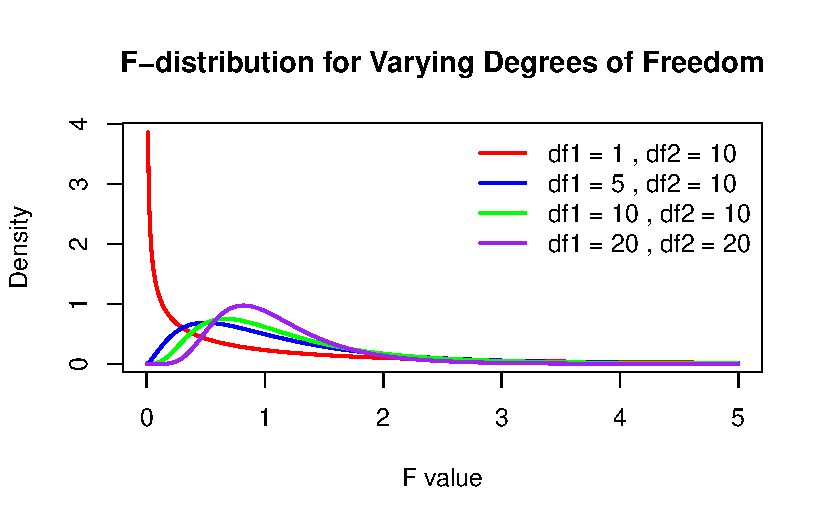
\includegraphics[keepaspectratio]{07_CRD_ANOVA_files/figure-pdf/unnamed-chunk-1-1.pdf}}

Key properties of the F-distribution:

\begin{itemize}
\tightlist
\item
  It is always non-negative: \(F \geq 0\).
\item
  It is asymmetric and skewed to the right, particularly for small
  degrees of freedom.
\item
  As the degrees of freedom increase, the F-distribution approaches a
  normal shape.
\end{itemize}

\section{Analysis of Variance for
CRD}\label{analysis-of-variance-for-crd}

Let's go back to the linear model for the single-factor CRD that we
examined earlier:

\[
Y_{ij} = \mu + A_i + e_{ij}
\]

where \(\mu\) is the overall mean, \(A_i\) are the treatment effects
(that is the difference between treatment means and the overall mean),
and \(e_{ij}\) are the error terms (the differences between the
observation and the fitted value, i.e.~treatment mean). Remember that
the estimated values for these parameters are the observed values:

\[
\begin{aligned}
\hat{\mu} &= \bar{Y}_{..} \\
\hat{A}_i &= \bar{Y}_{i.} - \bar{Y}_{..}\\
\hat{e}_{ij} &= Y_{ij} -  \bar{Y}_{i.}
\end{aligned}
\]

By taking \(\mu\) over to the left-hand-side in the equation, and
substituting the above observed values we obtain:

\[
\begin{aligned}
Y_{ij} - \mu &= (\mu_i - \mu) + (Y_{ij} - \mu)\\
Y_{ij} - \bar{Y} &= (\bar{Y}_i - \bar{Y}) + (Y_{ij} - \bar{Y}_i) \\
\end{aligned}
\]

Squaring and summing both sides gives the decomposition:

\[
\sum_i \sum_j (Y_{ij} - \bar{Y})^2 = \sum_i \sum_j (\bar{Y}_i - \bar{Y})^2 + \sum_i \sum_j (Y_{ij} - \bar{Y}_i)^2
\]

Each term represents squared deviations:

\begin{itemize}
\tightlist
\item
  The first term is of observations around the overall mean representing
  the total variation in the response.
\item
  The second is of the group means around the overall mean representing
  the explained variation or variation between treatments and,
\item
  The last term represents the deviations of observations from their
  treatment means (unexplained or within treatment variation).
\end{itemize}

We could also call these:

\[
SS_{\text{total}} = SS_{\text{between groups}} + SS_{\text{within groups}}
\] or

\[
SS_{\text{total}} = SS_{\text{treatment}} + SS_{\text{error}}
\]

\textbf{The analysis of variance is based on this identity}\footnote{In
  mathematics, an identity is an equation that is always true,
  regardless of the values of it's variables. In other words, the
  identity is true for all observations.}. The total sums of squares
equals the sum of squares between groups plus the sum of squares within
groups.

Back to our constructed example. What are the different sums of squares?
For Experiment 1, we get:
\(SS_{\text{total}} = 624; SS_{\text{between groups}} = 600; SS_{\text{within groups}} = 24\).
Verify these numbers and do the same for Experiment 2.

\section{ANOVA Table}\label{anova-table}

This division of the total sums of squares is typically summarised in an
analysis of variance table. The first column contains the ``source'' of
the variability with the first entry (the order is not important,
although this is the typical order) representing the between-treatment
variability (explained variation), second is the error (unexplained
variation, variation of experimental units within treatments) and lastly
the total variation. Here we have used the notation \(SS_A\) to
represent the sums of squares for treatment factor A. The second column
gives the sums of squares of each source. The third column contains the
degrees of freedom.

\begin{longtable}[]{@{}
  >{\raggedright\arraybackslash}p{(\linewidth - 8\tabcolsep) * \real{0.2000}}
  >{\raggedright\arraybackslash}p{(\linewidth - 8\tabcolsep) * \real{0.2000}}
  >{\raggedright\arraybackslash}p{(\linewidth - 8\tabcolsep) * \real{0.2000}}
  >{\raggedright\arraybackslash}p{(\linewidth - 8\tabcolsep) * \real{0.2000}}
  >{\raggedright\arraybackslash}p{(\linewidth - 8\tabcolsep) * \real{0.2000}}@{}}
\toprule\noalign{}
\begin{minipage}[b]{\linewidth}\raggedright
Source
\end{minipage} & \begin{minipage}[b]{\linewidth}\raggedright
Sums of Squares (SS)
\end{minipage} & \begin{minipage}[b]{\linewidth}\raggedright
df
\end{minipage} & \begin{minipage}[b]{\linewidth}\raggedright
Means Squares (MS)
\end{minipage} & \begin{minipage}[b]{\linewidth}\raggedright
F
\end{minipage} \\
\midrule\noalign{}
\endhead
\bottomrule\noalign{}
\endlastfoot
Treatment & \(\sum_i n_i(\bar{Y}_i - \bar{Y})^2\) & \(a-1\) &
\(MS_A = SS_A / (a-1)\) & \(MS_A / MSE\) \\
Residuals (Error) & \(\sum_i \sum_j (Y_{ij} - \bar{Y}_i)^2\) & \(N-a\) &
\(MSE = SSE / (N-a)\) & \\
Total & \(\sum_i \sum_j (Y_{ij} - \bar{Y})^2\) & \(N-1\) & & \\
\end{longtable}

The fourth column contains the Mean squares. This is what we get when we
divide sums of squares by the appropriate degrees of freedom.

\[ \text{MS} = \frac{SS}{df}\]

This is simply an average and may be seen as an estimate of variance. So
when we divide the treatment SS by its degrees of freedom, we get an
estimate of the variation due to treatments and similarly, for the the
residual SS, we get an estimate of the error variance. You've seen this
before!

\[\text{MSE} = \hat{\sigma}^2 = \frac{1}{N-a}\sum_i\sum_j(Y_{ij} - Y_{i.})^2\]

\subsection{What Are Degrees of
Freedom?}\label{what-are-degrees-of-freedom}

Degrees of freedom (df) represent the number of independent pieces of
information available for estimating a parameter. When making
statistical calculations, we typically lose one degree of freedom for
every estimated parameter before the current calculation.

For example, when estimating the standard deviation of a data set, we
first estimate the mean, thereby reducing the number of independent
observations available to calculate variability. This is why the
denominator in the variance formula is \(N-1\):

\[ s^2 = \frac{\sum(Y_i - \bar{Y})^2}{N -1} \]

You can think of degrees of freedom as the number of independent
deviations around a mean. If we have \(n\) observations and their mean,
once we know \(n-1\) of the values, the last one is fixed---it must take
on a specific value to satisfy the mean equation. Therefore, only
\(n-1\) observations are truly free to vary.

\textbf{Example: Three Numbers Summing to a Fixed Mean}

Say we have three (\(n=3\)) numbers: (4, 6, 8). The mean of these three
numbers is 6. If we only knew the first two numbers (4,6) and the mean,
the third number must be 8:

\[
\begin{aligned}
\bar{x} &= \frac{\sum x_i}{n}\\
6 &= \frac{4+6+x_3}{3}\\
18 &= 10 + x_3 \\
x_3 &= 8
\end{aligned}
\]

Since the third number is uniquely determined by the first two and the
mean, we only have \(n-1\) (i.e., 2) degrees of freedom.

\textbf{Another Intuitive Analogy}

Imagine you are distributing a fixed amount of money among friends. If
you have R100 and four friends, you can freely allocate money to three
friends, but whatever is left must go to the fourth friend to ensure the
total remains R100. Similarly, once the first \(n-1\) values are chosen,
the last value is determined, limiting the degrees of freedom.

\textbf{In ANOVA}

If you look at the treatment sums of squares:
\(\sum_i n_i (\bar{Y}_{i.} - \bar{Y}_{..})^2\). We have \(a\) deviations
around the grand mean. But once we know \(a-1\) of the treatment means
and the grand mean\footnote{Remember, \(\mu = \frac{\sum \mu_i}{a}\).},
the last mean is fixed. So we have \(a-1\) independent deviations around
the overall mean.

If you look at the treatment sums of squares:
\(\sum_i \sum_j (Y_{ij} - \bar{Y}_{..})^2\). We are using \(N\)
observations and calculating the deviations of these observations around
the overall mean. So, only \(N-1\) observations are free to vary, the
last observation is fixed for the calculated mean to hold true.

\section{Back to the constructed
example}\label{back-to-the-constructed-example}

What does the ANOVA table look like for our constructed example? You've
already worked out the sums of squares. What are the df's and Mean
squares?

Let's have a look at Experiment 1 first.

\begin{Shaded}
\begin{Highlighting}[]
\CommentTok{\# Experiment 1 data }
\NormalTok{exp1data }\OtherTok{\textless{}{-}} \FunctionTok{data.frame}\NormalTok{(}\AttributeTok{species =} \FunctionTok{rep}\NormalTok{(}\FunctionTok{c}\NormalTok{(}\StringTok{"A"}\NormalTok{,}\StringTok{"B"}\NormalTok{,}\StringTok{"C"}\NormalTok{), }\AttributeTok{each =} \DecValTok{3}\NormalTok{),}
                       \AttributeTok{response =} \FunctionTok{c}\NormalTok{(}\DecValTok{40}\NormalTok{,}\DecValTok{42}\NormalTok{,}\DecValTok{38}\NormalTok{,}\DecValTok{48}\NormalTok{,}\DecValTok{50}\NormalTok{,}\DecValTok{52}\NormalTok{,}\DecValTok{58}\NormalTok{,}\DecValTok{62}\NormalTok{,}\DecValTok{60}\NormalTok{))}

\NormalTok{exp1\_anova }\OtherTok{\textless{}{-}} \FunctionTok{aov}\NormalTok{(response}\SpecialCharTok{\textasciitilde{}}\NormalTok{species, }\AttributeTok{data =}\NormalTok{ exp1data)}
\FunctionTok{summary}\NormalTok{(exp1\_anova)}
\end{Highlighting}
\end{Shaded}

\begin{verbatim}
            Df Sum Sq Mean Sq F value   Pr(>F)    
species      2    600     300      75 5.69e-05 ***
Residuals    6     24       4                     
---
Signif. codes:  0 '***' 0.001 '**' 0.01 '*' 0.05 '.' 0.1 ' ' 1
\end{verbatim}

And then Experiment 2:

\begin{Shaded}
\begin{Highlighting}[]
\CommentTok{\# Experiment 2 data }
\NormalTok{exp2data }\OtherTok{\textless{}{-}} \FunctionTok{data.frame}\NormalTok{(}\AttributeTok{species =} \FunctionTok{rep}\NormalTok{(}\FunctionTok{c}\NormalTok{(}\StringTok{"A"}\NormalTok{,}\StringTok{"B"}\NormalTok{,}\StringTok{"C"}\NormalTok{), }\AttributeTok{each =} \DecValTok{3}\NormalTok{),}
                       \AttributeTok{response =} \FunctionTok{c}\NormalTok{(}\DecValTok{40}\NormalTok{,}\DecValTok{25}\NormalTok{,}\DecValTok{55}\NormalTok{,}\DecValTok{65}\NormalTok{,}\DecValTok{35}\NormalTok{,}\DecValTok{50}\NormalTok{,}\DecValTok{45}\NormalTok{,}\DecValTok{75}\NormalTok{,}\DecValTok{60}\NormalTok{))}

\NormalTok{exp2\_anova }\OtherTok{\textless{}{-}} \FunctionTok{aov}\NormalTok{(response}\SpecialCharTok{\textasciitilde{}}\NormalTok{species, }\AttributeTok{data =}\NormalTok{ exp2data)}
\FunctionTok{summary}\NormalTok{(exp2\_anova)}
\end{Highlighting}
\end{Shaded}

\begin{verbatim}
            Df Sum Sq Mean Sq F value Pr(>F)
species      2    600     300   1.333  0.332
Residuals    6   1350     225               
\end{verbatim}

Since the overall mean and the treatment means were the same in both
experiment, we expected the \(SS_{\text{treatment}}\) to be the same in
both experiments. This was indeed the case -- they are 600 in both
experiments. The sample sizes were also the same in both experiments, so
we would expect the df to be the same. With 9 observations, we have 8 df
in total. Three treatments (Species) leads to 2 treatment df and 6 df
remain for the residuals. The difference between the two experiments is
that the observations were much more variable in Experiment 2 than in
Experiment 1. Accordingly, we find that \(SS_{\text{error}}\) was much
larger in Experiment 2, and this led to larger MSE in Experiment 2. How
does this affect the conclusions we draw from each of the experiments?
This is where the F-ratio comes in.

\section{The F-test in ANOVA}\label{the-f-test-in-anova}

We first set up the null and alternate hypothesis. The null hypothesis
is that all treatments have the same mean, or equivalently, that all
treatment effects are zero.

\[
\begin{aligned}
H_0&: \mu_1 = \mu_2 = \ldots = \mu_a \\
H_0&: A_1 = A_2 = \ldots = A_a = 0\
\end{aligned}
\]

And the alternative hypothesis is the opposite of that:

\[
\begin{aligned}
H_A&: \text{At least one } \mu_i \text{ is different.} \\
H_A&: \text{At least one } A_i \neq 0
\end{aligned}
\]

\marginnote{\begin{footnotesize}

Read that again. The alternative is that at least one treatment is
different, there is a difference somewhere. It is not that all treatment
means are different.

\end{footnotesize}}

If \(H_0\) is true, the among-treatment-means variation should equal the
within-treatment variation. We can use the F-ratio to test \(H_0\):

\[ F^* = \frac{MS_A}{MSE} \]

This ratio has an F-distribution with \(a-1\) numerator degrees of
freedom and \(N-a\) denominator degrees of freedom.

You can think of the \emph{F-ratio} as a signal-to-noise ratio. If
\(H_0\) is true, \(F\) is expected to be close to 1. If \(H_0\) is
false, \(F\) is expected to be much larger than 1. This means that the
F-test we conduct is a \textbf{one-sided upper tailed test}. If \(H_0\)
is false, the means squares for treatment will be much larger than the
MSE, resulting in large F-values. We are only interested in this one
side of possible outcomes therefore, a one-sided test.

In Experiment 1, \(F = \frac{300}{4} = 75\), which leads to a very small
\(p\)-value (\(< 0.001\)). The signal was much larger than the noise,
and our data are very unlikely if \(H_0\) were true. So we have good
evidence that the treatments differ.

In Experiment 2, \(F = \frac{300}{225} = 1.33\), which leads to a large
\(p\)-value (\(0.33\)). Signal and noise were of similar magnitude, and
our data are not unlikely if \(H_0\) were true. So we have no evidence
against \(H_0\), i.e., no evidence that nitrate extraction differs
between species.

How did we get these p-values? This is the same as in any hypothesis
test. We have a test statistic and to say something about how likely
this test statistic (or more extreme is) under the null hypothesis, we
need the null distribution of the test statistic (that is the sampling
distribution of the test statistic as if the null hypothesis were true).
We then compared the observed value of the test statistic to that null
distribution and asked ourselves how unusual it is in light of that
distribution. Does our test statistic belong to this null distribution?

The \(F\) test statistic follows an F distribution as specified above.

\[\text{F}^* \sim \text{F}_{(a-1),\;(N-a)}\]

For both experiment, this equates to an F distribution with 2 numerator
and 6 denominator degrees of freedom which looks like this:

\begin{Shaded}
\begin{Highlighting}[]
\CommentTok{\# Define the range of F{-}values}
\NormalTok{x }\OtherTok{\textless{}{-}} \FunctionTok{seq}\NormalTok{(}\DecValTok{0}\NormalTok{, }\DecValTok{100}\NormalTok{, }\AttributeTok{length.out =} \DecValTok{500}\NormalTok{)}
\NormalTok{y }\OtherTok{\textless{}{-}} \FunctionTok{df}\NormalTok{(x, }\AttributeTok{df1 =} \DecValTok{2}\NormalTok{, }\AttributeTok{df2 =} \DecValTok{6}\NormalTok{)}
\FunctionTok{plot}\NormalTok{(x, y, }\AttributeTok{type=}\StringTok{"l"}\NormalTok{,}
     \AttributeTok{xlab=}\StringTok{"F value"}\NormalTok{, }\AttributeTok{ylab=}\StringTok{"Density"}\NormalTok{,}
     \AttributeTok{main=}\StringTok{""}\NormalTok{)}
\end{Highlighting}
\end{Shaded}

\pandocbounded{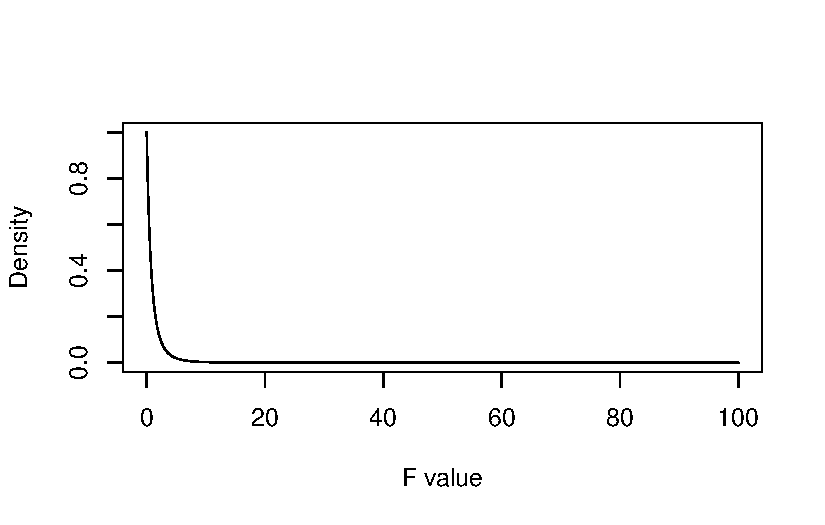
\includegraphics[keepaspectratio]{07_CRD_ANOVA_files/figure-pdf/unnamed-chunk-4-1.pdf}}

We can plot the test statistics on the graph as well and highlight the
area under the curve to the right of each of these test statistics:

\begin{Shaded}
\begin{Highlighting}[]
\CommentTok{\# Define x values}
\NormalTok{x }\OtherTok{\textless{}{-}} \FunctionTok{seq}\NormalTok{(}\DecValTok{0}\NormalTok{, }\DecValTok{100}\NormalTok{, }\AttributeTok{length.out =} \DecValTok{500}\NormalTok{)}
\NormalTok{y }\OtherTok{\textless{}{-}} \FunctionTok{df}\NormalTok{(x, }\AttributeTok{df1 =} \DecValTok{2}\NormalTok{, }\AttributeTok{df2 =} \DecValTok{6}\NormalTok{)}

\CommentTok{\# Define test\_stats}
\NormalTok{test\_stats }\OtherTok{\textless{}{-}} \FunctionTok{c}\NormalTok{(}\DecValTok{75}\NormalTok{, }\FloatTok{1.33}\NormalTok{)}

\CommentTok{\# Plot the F{-}distribution density curve}
\FunctionTok{plot}\NormalTok{(x, y, }\AttributeTok{type =} \StringTok{"l"}\NormalTok{, }\AttributeTok{col =} \StringTok{"black"}\NormalTok{, }\AttributeTok{lwd =} \DecValTok{2}\NormalTok{,}
     \AttributeTok{xlab =} \StringTok{"F value"}\NormalTok{, }\AttributeTok{ylab =} \StringTok{"Density"}\NormalTok{,}
     \AttributeTok{main =} \StringTok{""}\NormalTok{)}

\CommentTok{\# Add vertical lines at test\_stats}
\FunctionTok{abline}\NormalTok{(}\AttributeTok{v =}\NormalTok{ test\_stats, }\AttributeTok{col =} \StringTok{"red"}\NormalTok{, }\AttributeTok{lty =} \DecValTok{2}\NormalTok{, }\AttributeTok{lwd =} \DecValTok{2}\NormalTok{)}

\CommentTok{\# Shade the areas to the right of the test\_stats}
\FunctionTok{polygon}\NormalTok{(}\FunctionTok{c}\NormalTok{(test\_stats[}\DecValTok{1}\NormalTok{], x[x }\SpecialCharTok{\textgreater{}=}\NormalTok{ test\_stats[}\DecValTok{1}\NormalTok{]], }\FunctionTok{max}\NormalTok{(x)), }
        \FunctionTok{c}\NormalTok{(}\DecValTok{0}\NormalTok{, y[x }\SpecialCharTok{\textgreater{}=}\NormalTok{ test\_stats[}\DecValTok{1}\NormalTok{]], }\DecValTok{0}\NormalTok{), }\AttributeTok{col =} \FunctionTok{rgb}\NormalTok{(}\DecValTok{0}\NormalTok{, }\DecValTok{0}\NormalTok{, }\DecValTok{1}\NormalTok{, }\FloatTok{0.3}\NormalTok{), }\AttributeTok{border =} \ConstantTok{NA}\NormalTok{)}

\FunctionTok{polygon}\NormalTok{(}\FunctionTok{c}\NormalTok{(test\_stats[}\DecValTok{2}\NormalTok{], x[x }\SpecialCharTok{\textgreater{}=}\NormalTok{ test\_stats[}\DecValTok{2}\NormalTok{]], }\FunctionTok{max}\NormalTok{(x)), }
        \FunctionTok{c}\NormalTok{(}\DecValTok{0}\NormalTok{, y[x }\SpecialCharTok{\textgreater{}=}\NormalTok{ test\_stats[}\DecValTok{2}\NormalTok{]], }\DecValTok{0}\NormalTok{), }\AttributeTok{col =} \FunctionTok{rgb}\NormalTok{(}\DecValTok{1}\NormalTok{, }\DecValTok{0}\NormalTok{, }\DecValTok{0}\NormalTok{, }\FloatTok{0.3}\NormalTok{), }\AttributeTok{border =} \ConstantTok{NA}\NormalTok{)}

\CommentTok{\# Add points at the critical values}
\FunctionTok{points}\NormalTok{(test\_stats, }\FunctionTok{df}\NormalTok{(test\_stats, }\AttributeTok{df1 =} \DecValTok{2}\NormalTok{, }\AttributeTok{df2 =} \DecValTok{6}\NormalTok{), }\AttributeTok{pch =} \DecValTok{19}\NormalTok{, }\AttributeTok{col =} \StringTok{"black"}\NormalTok{)}
\end{Highlighting}
\end{Shaded}

\pandocbounded{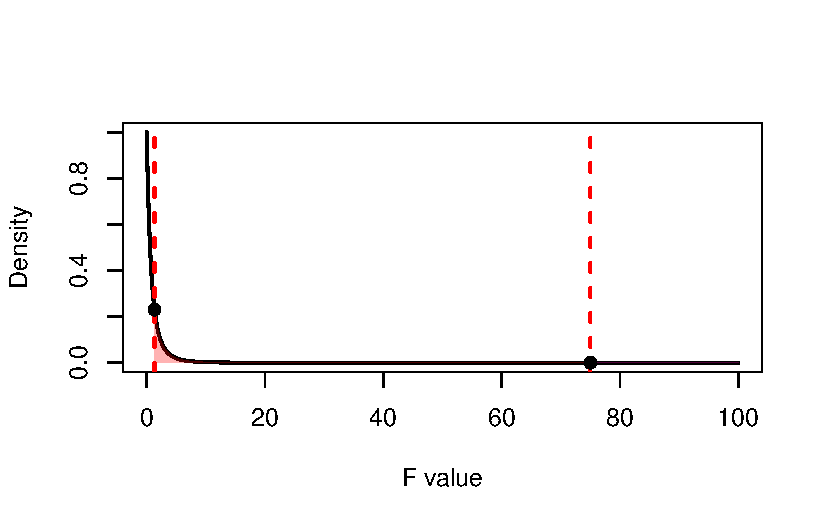
\includegraphics[keepaspectratio]{07_CRD_ANOVA_files/figure-pdf/unnamed-chunk-5-1.pdf}}

Remember sampling distributions are probability distributions. For
continuous random variables, the area under the curve represents
probability. Specifically, the probability of a random variable taking
on a specific value or larger, is the area under the curve to the right
of that value. For test statistics and their probability distribution,
that probability is the p-value. The p-value is the probability of
observing a test statistic at least as extreme as we did if the null
hypothesis was in fact true. The smaller the p-value, the stronger the
evidence against \(H_0\).

We can obtain the p-value in two ways (you will need to be able to do
both):

\begin{enumerate}
\def\labelenumi{\arabic{enumi}.}
\tightlist
\item
  Using Software.
\end{enumerate}

In R, there are several built-in functions for certain probability
distributions. These functions typically follow a naming convention:

\begin{itemize}
\tightlist
\item
  \texttt{d\textless{}dist\textgreater{}()} for density functions
\item
  \texttt{p\textless{}dist\textgreater{}()} for cumulative probability
  functions
\item
  \texttt{q\textless{}dist\textgreater{}()} for quantile functions
\item
  \texttt{r\textless{}dist\textgreater{}()} for random sampling
\end{itemize}

For example, when working with the F-distribution, we use:

\begin{itemize}
\tightlist
\item
  \texttt{df(x,\ df1,\ df2)} for the probability density function (PDF)
\item
  \texttt{pf(x,\ df1,\ df2)} for the cumulative distribution function
  (CDF)
\item
  \texttt{qf(p,\ df1,\ df2)} for quantiles
\item
  \texttt{rf(n,\ df1,\ df2)} for random sampling
\end{itemize}

To obtain a p-value, we often use the cumulative probability functions
(\texttt{p\textless{}dist\textgreater{}()}) with returns \(Pr[X<x]\) so
\(Pr[X>x] = 1 - Pr[X<x]\). Below is how to obtain the p-value for the
second experiment:

\begin{Shaded}
\begin{Highlighting}[]
\NormalTok{f\_statistic }\OtherTok{\textless{}{-}} \FloatTok{1.33}
\NormalTok{df1 }\OtherTok{\textless{}{-}} \DecValTok{2}  \CommentTok{\# Numerator degrees of freedom}
\NormalTok{df2 }\OtherTok{\textless{}{-}} \DecValTok{6}  \CommentTok{\# Denominator degrees of freedom}

\CommentTok{\# Upper{-}tail probability (right{-}tailed test)}
\NormalTok{p\_value }\OtherTok{\textless{}{-}} \DecValTok{1} \SpecialCharTok{{-}} \FunctionTok{pf}\NormalTok{(f\_statistic, df1, df2)}
\NormalTok{p\_value}
\end{Highlighting}
\end{Shaded}

\begin{verbatim}
[1] 0.332583
\end{verbatim}

This value is quite large and corresponds to the area to the right of an
F value of 1.33 for the distribution above. We interpret this p-value as
the test statistic is quite likely to have come from this null
distribution, there is a 33\% chance of observing this test statistic or
more extreme if the null hypothesis is true. We do not have strong
evidence against the null hypothesis of equal means.

\begin{tcolorbox}[enhanced jigsaw, opacitybacktitle=0.6, colbacktitle=quarto-callout-caution-color!10!white, toprule=.15mm, bottomtitle=1mm, breakable, leftrule=.75mm, rightrule=.15mm, left=2mm, colback=white, coltitle=black, toptitle=1mm, colframe=quarto-callout-caution-color-frame, bottomrule=.15mm, title=\textcolor{quarto-callout-caution-color}{\faFire}\hspace{0.5em}{Caution}, arc=.35mm, titlerule=0mm, opacityback=0]

A large p-value does not mean that \(H_0\) is true!

\begin{itemize}
\tightlist
\item
  The p-value is not the probability that the null hypothesis is true.
\item
  The p-value is not the probability that the alternative hypothesis is
  false.
\item
  The p-value is a statement about the relation of the data to the null
  hypothesis.
\item
  The p-value does not indicate the size or biological importance of the
  observed pattern.
\end{itemize}

\end{tcolorbox}

\begin{tcolorbox}[enhanced jigsaw, opacitybacktitle=0.6, colbacktitle=quarto-callout-tip-color!10!white, toprule=.15mm, bottomtitle=1mm, breakable, leftrule=.75mm, rightrule=.15mm, left=2mm, colback=white, coltitle=black, toptitle=1mm, colframe=quarto-callout-tip-color-frame, bottomrule=.15mm, title=\textcolor{quarto-callout-tip-color}{\faLightbulb}\hspace{0.5em}{Tip}, arc=.35mm, titlerule=0mm, opacityback=0]

You can round the p-value if you need to enter the value to a certain
number of decimals in a quiz or test using the function \texttt{round}.

\end{tcolorbox}

\begin{enumerate}
\def\labelenumi{\arabic{enumi}.}
\setcounter{enumi}{1}
\tightlist
\item
  Using tables.
\end{enumerate}

Before the days of widespread programming, statisticians used tables to
find critical values and p-values for various probability distributions.
These tables were pre-computed for different significance levels (e.g.,
0.05, 0.01) and degrees of freedom. In modern statistical analysis, we
no longer rely on static tables, as software like R can compute exact
probabilities. But since we have written examinations, we have to learn
how to do this and it is a useful exercise to make sure you understand
what you are doing and not just spitting out a value.

F-tables look like this:

\pandocbounded{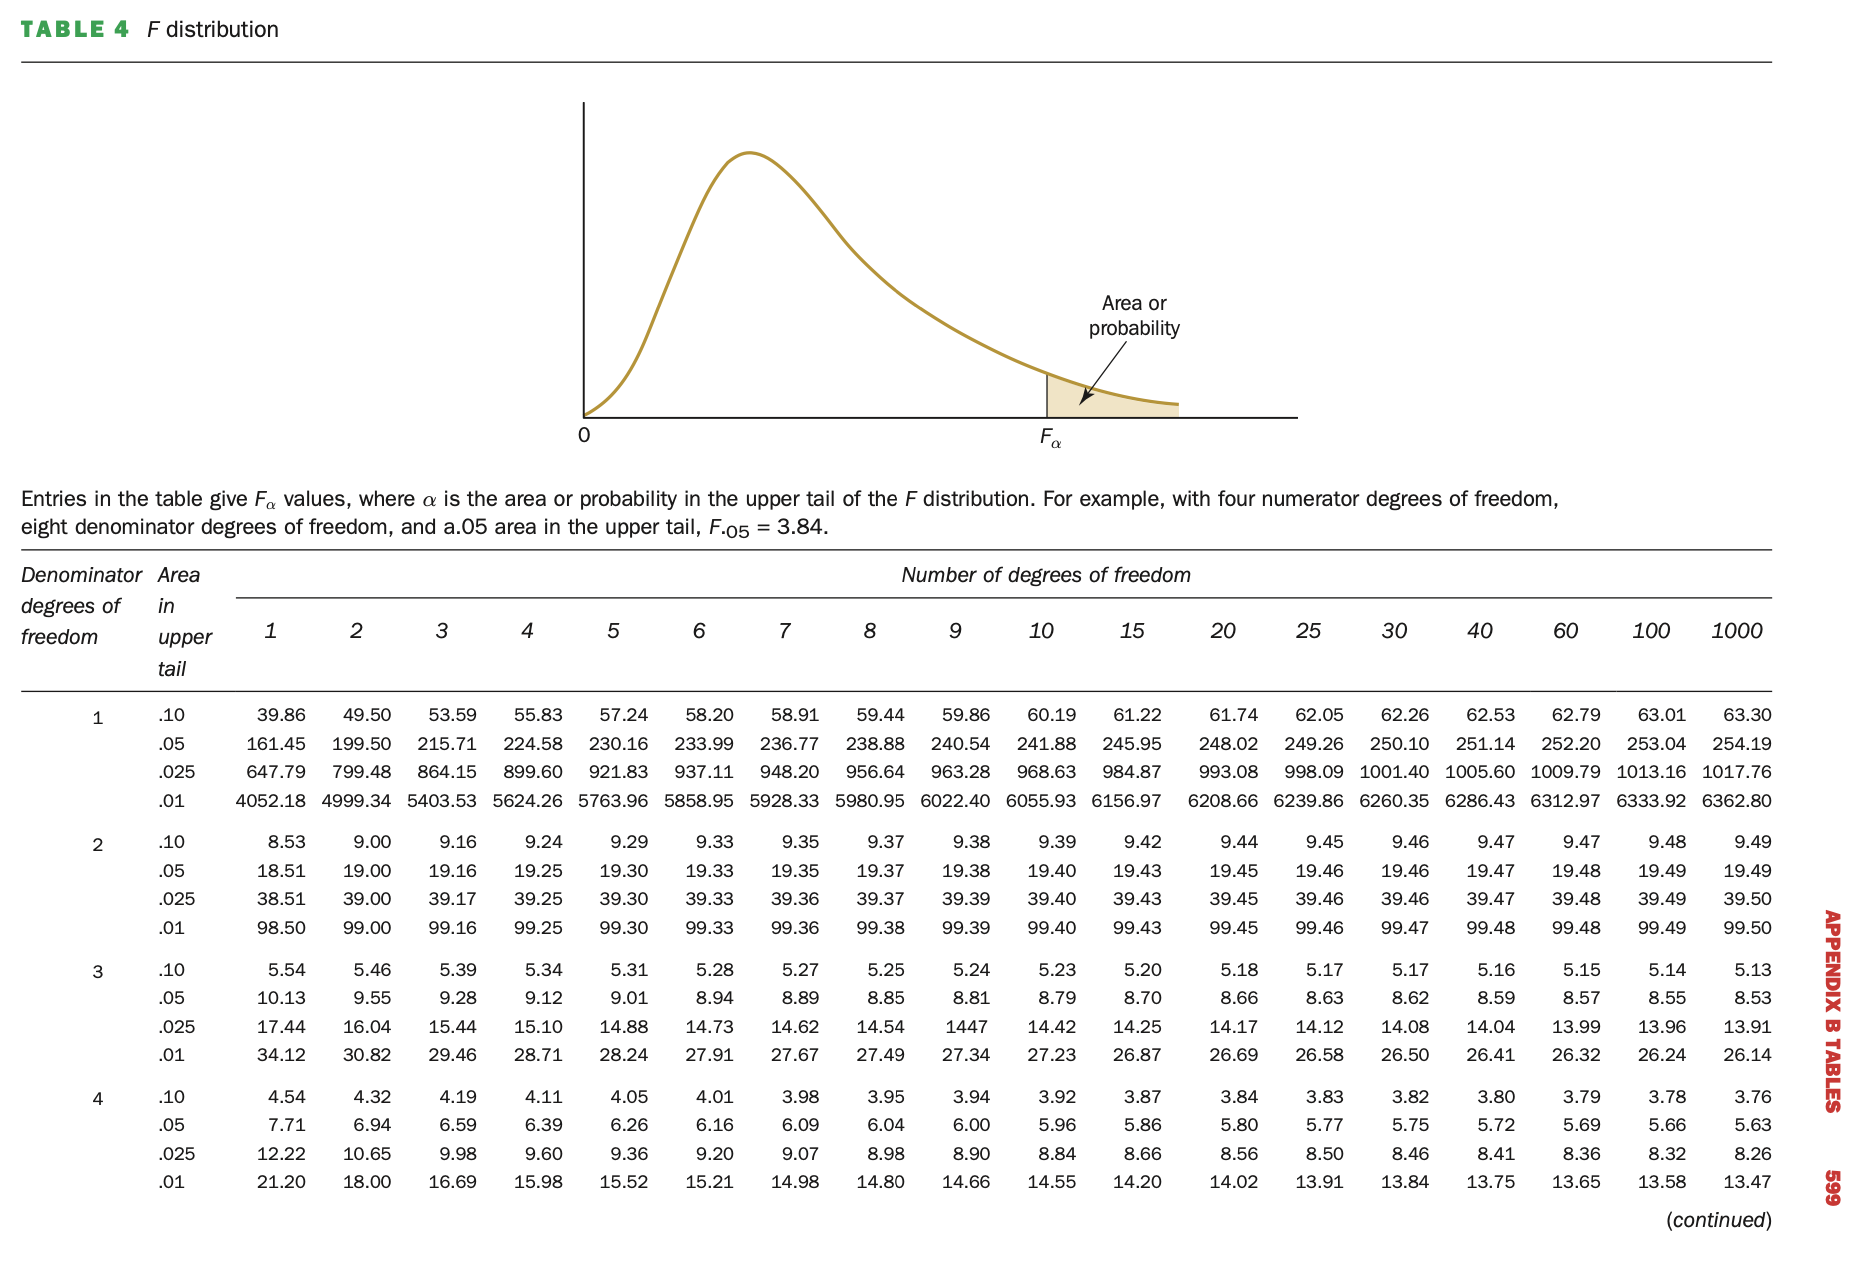
\includegraphics[keepaspectratio]{images/fdist1.png}}

Read it carefully. The table says: ``Entries in the table give
\(F_\alpha\) values, where \(\alpha\) is the area or probability in the
upper tail of the F distribution. For example, with four numerator
degrees of freedom, eight denominator degrees of freedom, and 0.05 area
in the upper tail, F.05 = 3.84.'' This is important, not all tables look
like this. See if you can find the F-value mentioned.

The numerator df is in the column and the denominator df is in the row.
In the row dimension are different \(\alpha\) values as well. To find an
F-value, locate the df in the column and row. Can you find the
following:

\begin{itemize}
\tightlist
\item
  \(F_{4,4}^{0.05} = 6.39\)
\item
  \(F_{10,2}^{0.1} = 9.39\)
\item
  \(F_{1,1}^{0.025} = 647.79\)
\item
  \(F_{7,3}^{0.01} = 27.67\)
\end{itemize}

This is how we find critical values of F-distributions. If you are asked
to compare a test statistic with a critical value at a specific
significance level, you will find the value with a table like this. To
find the critical values in R, we use the \texttt{fq} function:

\begin{Shaded}
\begin{Highlighting}[]
\CommentTok{\# F4,4 0.05}

\FunctionTok{qf}\NormalTok{(}\AttributeTok{p =} \FloatTok{0.05}\NormalTok{, }\AttributeTok{df1 =} \DecValTok{4}\NormalTok{, }\AttributeTok{df2 =} \DecValTok{4}\NormalTok{, }\AttributeTok{lower.tail =} \ConstantTok{FALSE}\NormalTok{) }\CommentTok{\# if lower.tail = TRUE which is the default, the critical value with probability 0.05 to the left would be return. }
\end{Highlighting}
\end{Shaded}

\begin{verbatim}
[1] 6.388233
\end{verbatim}

\begin{Shaded}
\begin{Highlighting}[]
\CommentTok{\# F10,2 0.11}
\FunctionTok{qf}\NormalTok{(}\AttributeTok{p =} \FloatTok{0.1}\NormalTok{,   }\AttributeTok{df1 =} \DecValTok{10}\NormalTok{, }\AttributeTok{df2 =} \DecValTok{2}\NormalTok{, }\AttributeTok{lower.tail =} \ConstantTok{FALSE}\NormalTok{)}
\end{Highlighting}
\end{Shaded}

\begin{verbatim}
[1] 9.391573
\end{verbatim}

\begin{Shaded}
\begin{Highlighting}[]
\CommentTok{\# F1,1 0.025}
\FunctionTok{qf}\NormalTok{(}\AttributeTok{p =} \FloatTok{0.025}\NormalTok{, }\AttributeTok{df1 =} \DecValTok{1}\NormalTok{,  }\AttributeTok{df2 =} \DecValTok{1}\NormalTok{, }\AttributeTok{lower.tail =} \ConstantTok{FALSE}\NormalTok{)}
\end{Highlighting}
\end{Shaded}

\begin{verbatim}
[1] 647.789
\end{verbatim}

\begin{Shaded}
\begin{Highlighting}[]
\CommentTok{\# F7,3 0.01}
\FunctionTok{qf}\NormalTok{(}\AttributeTok{p =} \FloatTok{0.01}\NormalTok{,  }\AttributeTok{df1 =} \DecValTok{7}\NormalTok{,  }\AttributeTok{df2 =} \DecValTok{3}\NormalTok{, }\AttributeTok{lower.tail =} \ConstantTok{FALSE}\NormalTok{)}
\end{Highlighting}
\end{Shaded}

\begin{verbatim}
[1] 27.6717
\end{verbatim}

Now, how do we use the tables to obtain p-values? The test statistic for
the first Experiment was 1.33 and the df's were 2 (num) and 6 (denom).
If we look at the table above, it only goes to 4 denominator degrees of
freedom, so we need the continuation of the table.

\pandocbounded{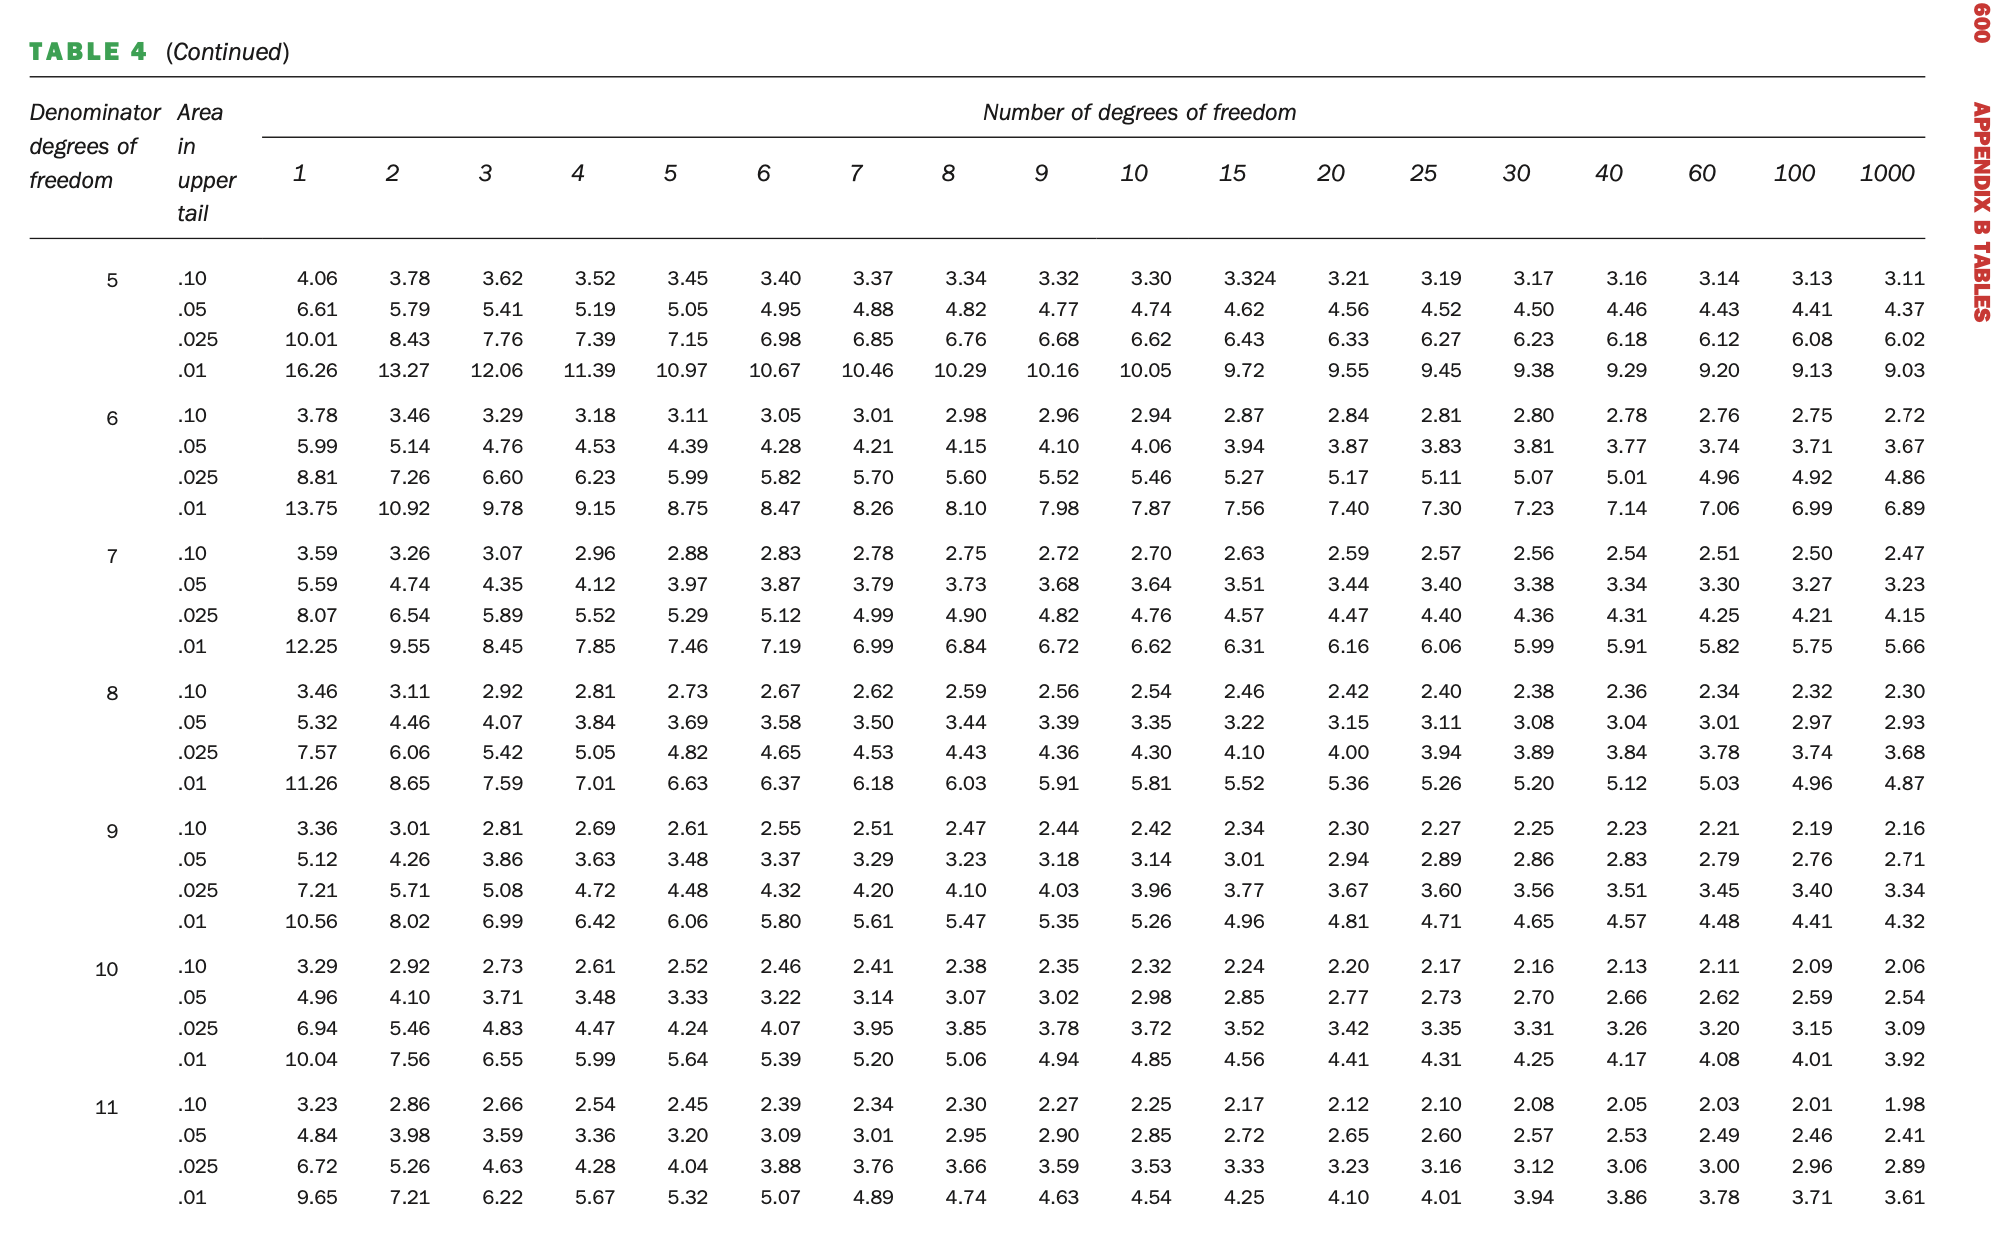
\includegraphics[keepaspectratio]{images/fdist2.png}}Now
we locate the F-values with 2 and 6 degrees of freedom and compare the
test statistic of the second experiment (1.33) to them. The smallest
value is 3.46 where the probability to the right of that value is 0.1.
Our test statistic is much smaller than this, so lies further to the
right and so logically, the right-hand-side probability of this value
with be greater than 0.1. So we conclude that the p-value that our
p-value is \textgreater{} 0.1 (which it is, we calculated it to be
0.32). With tables we cannot get exact probabilities, but we can say
something about the magnitude of the p-value. Try it for the first
experiment which had an F-value of 75.

\section{Conclusion: Does social media multitasking impact academic
performance of
students?}\label{conclusion-does-social-media-multitasking-impact-academic-performance-of-students}

Let's revisit the real experiment we started this section with. I repeat
the experiment description below.

\begin{tcolorbox}[enhanced jigsaw, opacitybacktitle=0.6, colbacktitle=quarto-callout-warning-color!10!white, toprule=.15mm, bottomtitle=1mm, breakable, leftrule=.75mm, rightrule=.15mm, left=2mm, colback=white, coltitle=black, toptitle=1mm, colframe=quarto-callout-warning-color-frame, bottomrule=.15mm, title={Example 5.1}, arc=.35mm, titlerule=0mm, opacityback=0]

Two researchers from Turkey, Demirbilek and Talan
(\citeproc{ref-multitask2018}{2018}), conducted a study to try and
answer this question. Specifically, they examined the impact of social
media multitasking during live lectures on students' academic
performance.

A total of 120 undergraduate students were randomly assigned to one of
three groups:

\begin{enumerate}
\def\labelenumi{\arabic{enumi}.}
\tightlist
\item
  \textbf{Control Group:} Students used traditional pen-and-paper
  note-taking.
\item
  \textbf{Experimental Group 1 (Exp 1):} Students engaged in SMS texting
  during the lecture.
\item
  \textbf{Experimental Group 2 (Exp 2):} Students used Facebook during
  the lecture.
\end{enumerate}

Over a three-week period, participants attended the same lectures on
Microsoft Excel. To measure academic performance, a standardised test
was administered.

\end{tcolorbox}

In the previous sections we introduced this study, checked the model
assumptions and obtained estimates of the model parameters. Now equipped
with that information and all that you have learnt, we are ready to fit
to conduct the ANOVA hypothesis test to finally answer our question:

Does social media multitasking impact academic performance of students?

We start with the hypotheses:

\[H_0: \mu_1 = \mu_2 = \ldots = \mu_a\]

In words we say that the average academic performance of students did
not differ across the treatments (levels of social media multitasking).

And the alternative hypothesis is the opposite of that:

\[H_A: \text{At least one } \mu_i \text{ is different.}\]

At least one of the social media multitasking treatments resulted in a
different mean academic performance, they are not all equal.

We have fit the model already (called \texttt{m1}) and call the
\texttt{summary} function to obtain the ANOVA table:

\begin{Shaded}
\begin{Highlighting}[]
\CommentTok{\# m1 \textless{}{-} aov(Posttest \textasciitilde{} Group, data = multitask)}

\FunctionTok{summary}\NormalTok{(m1)}
\end{Highlighting}
\end{Shaded}

\begin{verbatim}
             Df Sum Sq Mean Sq F value   Pr(>F)    
Group         2  10975    5488   27.42 1.72e-10 ***
Residuals   117  23417     200                     
---
Signif. codes:  0 '***' 0.001 '**' 0.01 '*' 0.05 '.' 0.1 ' ' 1
\end{verbatim}

Violà! We have our ANOVA table. Inspect the results and make sure you
understand how each value is obtained and what they represent. By just
looking at the table, you should be able to answer the following
questions:

\begin{enumerate}
\def\labelenumi{\arabic{enumi}.}
\tightlist
\item
  How many treatments were there?
\item
  How many observations in total?
\item
  Is there evidence for a treatment effect?
\end{enumerate}

The first two you can answer with the degrees of freedom and the third
is answered by conducting the hypothesis test. With three treatments, we
have 2 treatment degrees of freedom. We had 40 students per group, the
sample size is then 120 which means there are 117 degrees of freedom for
the residuals. The treatment MS (5488) was much larger that the MSE
(200). This leads to an F-ratio of 27.42 with a p-value of
\(1.72\times e^{-10}\) (that's extremely small). We have strong evidence
that the treatments did result different academic performances across
students At least one treatment resulted in a different mean academic
performance. In a report, you would write:

``The manipulation of social media multitasking affected the academic
performance of students in this experiment (\(F_{2,117} = 27.42\),
\(p=1.72\times e^{-10}\)).''

But which treatments differed? \textbf{We cannot answer that question
with this hypothesis.} It only tells us that there is a difference,
there is a treatment effect. \textbf{It does not tell us where the
difference or possible differences lie.} To determine this, we need to
use treatment contrasts. Before we do this or present any results, we
need to do one last thing.

\section{Model Checking}\label{model-checking}

Remember that we said some of our assumptions need to be checked after
the model is fitted. Our model specifies the error terms are (1)
normally distributed, (2) all with the same variance (homoscedastic),
and (3) that they are independent. The residuals are estimates of these
error terms and we can therefore use them to check the model
assumptions. Normally distributed, equal variance and independent really
means that there is no discernible pattern or structure left in the
residuals. If there is, then the model has failed to pick up an
important structure in the data.\footnote{The same concepts apply to
  linear regression models.}

We call the function \texttt{plot} on our model object. For our purposes
we are only going to look at two of the plots and we inspect them one by
one by specifying the plot number with the argument \texttt{which}:

\begin{Shaded}
\begin{Highlighting}[]
\FunctionTok{plot}\NormalTok{(m1, }\AttributeTok{which =} \DecValTok{1}\NormalTok{)}
\end{Highlighting}
\end{Shaded}

\pandocbounded{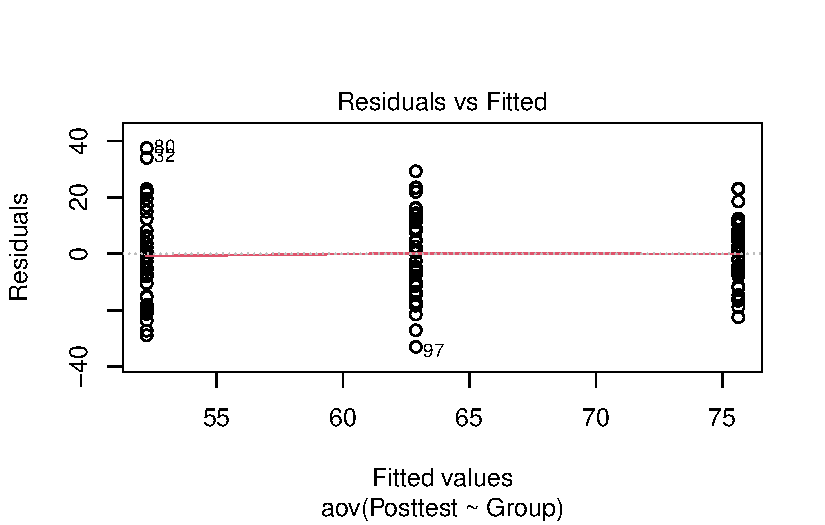
\includegraphics[keepaspectratio]{07_CRD_ANOVA_files/figure-pdf/unnamed-chunk-9-1.pdf}}

This is a plot of the residuals (obs - fitted) against the fitted values
and we are hoping to see no patterns. We have three lines, one for each
treatment group and we want to check that our residuals are centered
around zero and have constant variance across the groups. \footnote{Remember
  we assumed \(e_{ij} \sim N(0,\sigma^2)\) and residuals are estimates
  of the errors.}

\begin{Shaded}
\begin{Highlighting}[]
\FunctionTok{plot}\NormalTok{(m1, }\AttributeTok{which =} \DecValTok{2}\NormalTok{)}
\end{Highlighting}
\end{Shaded}

\pandocbounded{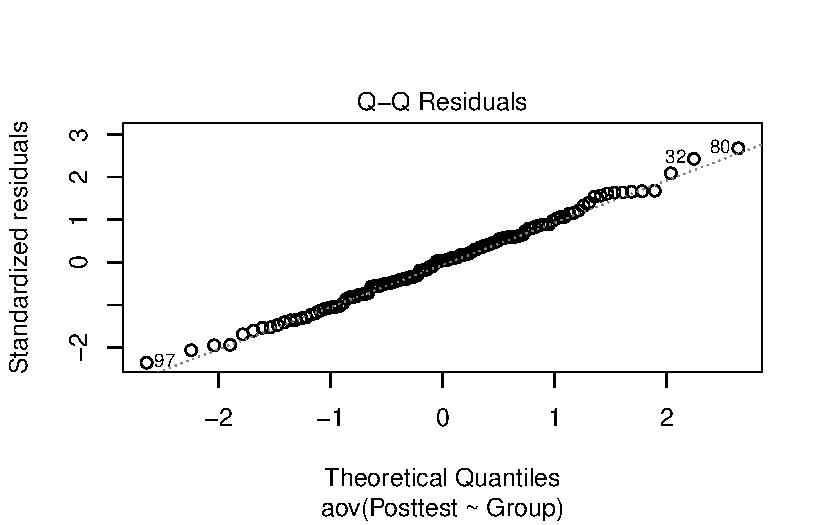
\includegraphics[keepaspectratio]{07_CRD_ANOVA_files/figure-pdf/unnamed-chunk-10-1.pdf}}

The second plot is a Q-Q plot which we have seen before when we checked
the assumption of normality before model fitting. Now, we plot the
standardised residuals against the theoretical quantiles of a standard
normal distribution. We are looking for the same pattern as before, that
the points fall close to the dotted line. As usual, there many be some
deviations at the tails but for the most part, there are no serious
problems with this plot. If there is some doubt, we can also look at a
histogram of the residuals:

\begin{Shaded}
\begin{Highlighting}[]
\FunctionTok{hist}\NormalTok{(}\FunctionTok{resid}\NormalTok{(m1))}
\end{Highlighting}
\end{Shaded}

\pandocbounded{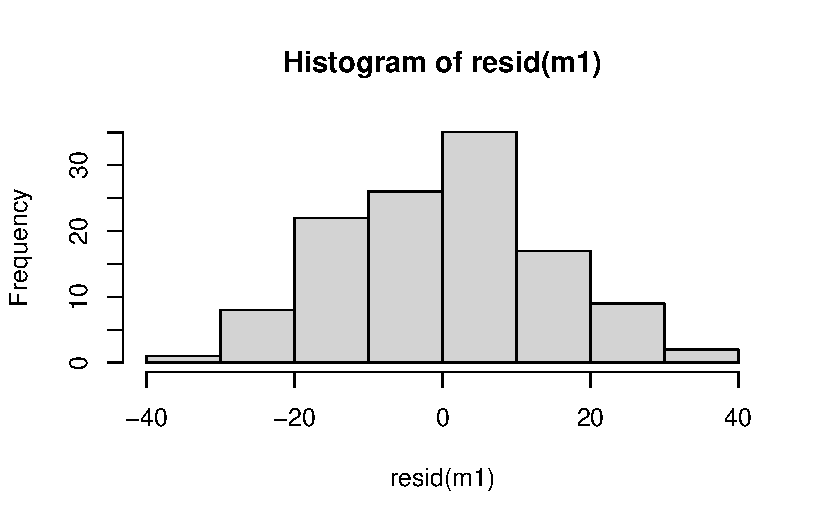
\includegraphics[keepaspectratio]{07_CRD_ANOVA_files/figure-pdf/unnamed-chunk-11-1.pdf}}

The assumption of independent errors is mostly checked before model
fitting and by consideration of the experimental design. If we suspected
auto-correlated residuals, we could plot the residuals against order:

\begin{Shaded}
\begin{Highlighting}[]
\FunctionTok{plot}\NormalTok{(}\FunctionTok{resid}\NormalTok{(m1) }\SpecialCharTok{\textasciitilde{}} \FunctionTok{seq\_along}\NormalTok{(}\FunctionTok{resid}\NormalTok{(m1)), }
     \AttributeTok{xlab =} \StringTok{"Order of Observations"}\NormalTok{, }
     \AttributeTok{ylab =} \StringTok{"Residuals"}\NormalTok{, }
     \AttributeTok{main =} \StringTok{"Residuals vs. Order"}\NormalTok{)}
\FunctionTok{abline}\NormalTok{(}\AttributeTok{h =} \DecValTok{0}\NormalTok{, }\AttributeTok{col =} \StringTok{"red"}\NormalTok{)}
\end{Highlighting}
\end{Shaded}

\pandocbounded{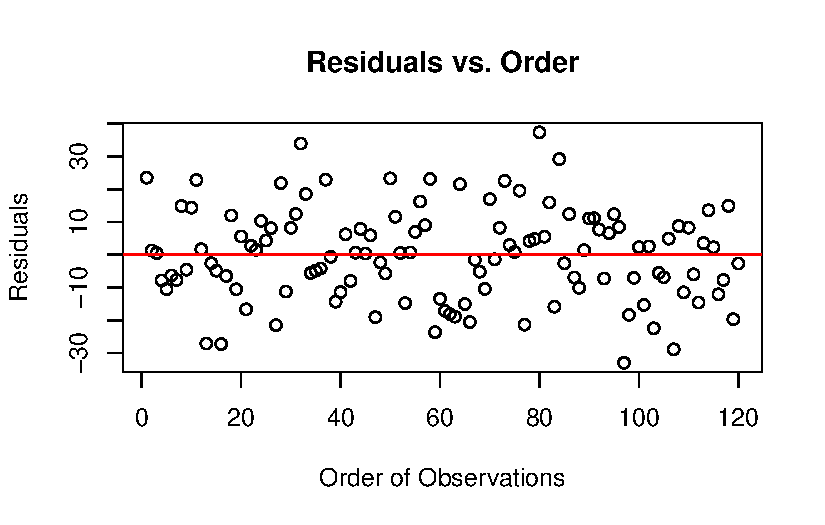
\includegraphics[keepaspectratio]{07_CRD_ANOVA_files/figure-pdf/unnamed-chunk-12-1.pdf}}

There are no patterns at all, the residuals appear randomly distributed.
So no indications of dependence.

\section{Summary}\label{summary-2}

That's a lot. So let's summarise what we did in this chapter:

We introduced Analysis of Variance (ANOVA), which is fundamentally the
same as a regression model with categorical variables but parameterised
differently. ANOVA allows us to partition total variance into
between-treatment and within-treatment variability, helping us determine
whether observed differences in the response variable are due to the
treatments and not just sampling error.

We explored ANOVA through a constructed experiment on nitrate removal by
plants, demonstrating that variation within treatments influences our
ability to detect true treatment effects. The F-ratio, a measure of the
signal-to-noise ratio, is central to ANOVA. A large F-ratio suggests
that between-group variability is greater than within-group variability,
providing evidence that at least one treatment differs.

The F-test determines statistical significance, and its p-value is
derived from the F-distribution. A small p-value suggests strong
evidence against the null hypothesis (\(H_0\)), indicating at least one
group mean differs. The ANOVA table summarises the calculations of the
hypothesis test, including sums of squares (SS), degrees of freedom
(df), mean squares (MS), and the F-statistic.

Applying ANOVA to real experimental data, we analysed the impact of
social media multitasking on student performance. With three treatment
groups (control, SMS, Facebook), we found a statistically significant
effect (\(F_{2,117} = 27.42\), \(p=1.72\times10^{-10}\)), confirming
that at least one treatment influenced academic performance. However,
ANOVA does not specify which groups differ and how they differ --- this
requires post-hoc tests.

Finally, we validated model assumptions:

\begin{itemize}
\item
  Normality: Checked via a Q-Q plot and histogram of residuals.
\item
  Homoscedasticity (equal variance): Examined using a residuals
  vs.~fitted plot.
\item
  Independence: Considered in the experimental design and checked by
  plotting residuals against observation order.
\end{itemize}

\chapter{Contrasts}\label{contrasts}

The aim in many experiments is to compare treatments. To do this we
contrast one group of means with another, i.e.~we compare means, or
groups of means, to see if treatments differ, and by how much they
differ. A comparison of treatments (or groups of treatments) is called a
contrast. If the experiment has been conducted as a result of specific
research hypotheses, these will already define the contrasts we should
construct first.

For a single-factor CRD with only two treatments, we could conduct a
t-test to compare the two means or construct a confidence interval to
estimate the difference. But we know that with more than two treatments,
we encounter problems of multiple testing. How do we contrast treatments
when we have a factor with more than two levels?

\section*{Contrasting pairs of treatment
means}\label{contrasting-pairs-of-treatment-means}
\addcontentsline{toc}{section}{Contrasting pairs of treatment means}

\markright{Contrasting pairs of treatment means}

We wrote the ANOVA model as:

\[Y_{ij} = \mu + A_i + e_{ij}\]

with overall mean and the treatment effects as the parameters (as well
as the error variance). Because the effects are constrained to sum to
zero, i.e.~\(\sum_i^a A_i = 0\) we call this ANOVA model the
\emph{sum-to-zero} parameterisation.

The above parameterisation is useful for constructing ANOVA tables. For
estimating differences between treatments, however, a different
parameterisation is more useful:

\[Y_{ij} = A_i + e_{ij}\] In this version, we no longer have the overall
mean as a parameter but use only the treatment effects \(A_i\). Remember
that any model ultimately needs to describe the treatment means. There
are a number of different ways in which to do this. One is the so-called
\emph{treatment contrast} parameterisation, which R uses as default for
regression models. In this parameterisation, \(A_1\) estimates the mean
of the baseline treatment (by default, R orders the treatments
alphabetically and takes the first one as baseline). The other
parameters then estimate the difference between each treatment and the
baseline treatment: \(A_2\) estimates the difference between the second
and the first treatment, \(A_3\) estimates the difference between the
third and the first, etc.

\marginnote{\begin{footnotesize}

Construction of treatmenat means under the \emph{treatment contrast}
parameterisation:

\[
\begin{aligned}
\mu_1 &= A_1 \\ 
\mu_2 &= A_1 + A_2 \\
\vdots& \\
\mu_a &= A_1 + A_a
\end{aligned}
\]

and under the \emph{sum-to-zero} parameterisation:

\[
\begin{aligned}
\mu_1 &= \mu + A_1 \\ 
\mu_2 &= \mu + A_2 \\
\vdots& \\
\mu_a &= \mu + A_a
\end{aligned}
\]

\end{footnotesize}}

To get a better understanding of this, let's fit the model to the social
media data with this parameterisation. In R, this is done by using the
\texttt{lm} function.

\begin{Shaded}
\begin{Highlighting}[]
\NormalTok{m1.tc }\OtherTok{\textless{}{-}} \FunctionTok{lm}\NormalTok{(Posttest }\SpecialCharTok{\textasciitilde{}}\NormalTok{ Group, }\AttributeTok{data =}\NormalTok{ multitask)}
\FunctionTok{summary}\NormalTok{(m1.tc)}
\end{Highlighting}
\end{Shaded}

\begin{verbatim}

Call:
lm(formula = Posttest ~ Group, data = multitask)

Residuals:
    Min      1Q  Median      3Q     Max 
-32.964 -10.175   0.583   8.550  37.408 

Coefficients:
            Estimate Std. Error t value Pr(>|t|)    
(Intercept)   75.634      2.237  33.812  < 2e-16 ***
GroupExp1    -12.752      3.163  -4.031 9.92e-05 ***
GroupExp2    -23.394      3.163  -7.395 2.32e-11 ***
---
Signif. codes:  0 '***' 0.001 '**' 0.01 '*' 0.05 '.' 0.1 ' ' 1

Residual standard error: 14.15 on 117 degrees of freedom
Multiple R-squared:  0.3191,    Adjusted R-squared:  0.3075 
F-statistic: 27.42 on 2 and 117 DF,  p-value: 1.717e-10
\end{verbatim}

This is exactly the same output as you have seen before in the
regression section! The intercept measures the mean of the baseline
treatment (here it is the Control group). The next estimate
\texttt{GroupExp1} is the difference between the mean of Experiment 1
and the mean of the Control group. Similarly, the last one is the
difference between the mean of the Control Group and that of Experiment
2. You can verify this by using the mean estimates we obtain when we fit
the model previously:

\begin{Shaded}
\begin{Highlighting}[]
\FunctionTok{model.tables}\NormalTok{(m1, }\AttributeTok{type =} \StringTok{"means"}\NormalTok{)}
\end{Highlighting}
\end{Shaded}

\begin{verbatim}
Tables of means
Grand mean
         
63.58527 

 Group 
Group
Control    Exp1    Exp2 
  75.63   62.88   52.24 
\end{verbatim}

\begin{Shaded}
\begin{Highlighting}[]
\FloatTok{62.88} \SpecialCharTok{{-}} \FloatTok{75.63} \CommentTok{\#GroupExp1}
\end{Highlighting}
\end{Shaded}

\begin{verbatim}
[1] -12.75
\end{verbatim}

\begin{Shaded}
\begin{Highlighting}[]
\FloatTok{52.24} \SpecialCharTok{{-}} \FloatTok{75.63} \CommentTok{\#GroupExp2 }
\end{Highlighting}
\end{Shaded}

\begin{verbatim}
[1] -23.39
\end{verbatim}

Why is this useful? Now, we can formally test whether these differences
are statistically significant using a hypothesis test!

Think back to regression---what was the null hypothesis for the
coefficients in the output?

It was:

\[\beta_i = 0\].

The same principle applies here. We test whether the treatment effects
(\(A_i\)) are equal to zero:

\[H_0: A_i = 0\]

Since we are interested in testing differences between groups, and the
control group serves as the baseline, we are specifically testing:

\[
\begin{aligned}
H_0: A_2 &= 0 \\ 
H_0: A_3 &= 0
\end{aligned}
\]

This is the test that R conducts in the output above. It tests, for the
last two parameters, the hypothesis that the difference between
Experiment 1 and the Control is zero an that the difference between
Experiment 2 and the Control is zero. In both cases, the p-values are
extremely small which suggest that there are differences (the effects
are not equal to zero).

What about the intercept? This is testing that the mean of the Control
group is zero. So, it tests whether the students in the control group
scored zero on average. This doesn't really make sense and it is not a
useful test. So not all tests that R carries out are necessarily useful
or informative! Very often testing whether the intercept is different
from zero is not interesting.

What if we aren't interested in the contrast R perform by default? We
wanted to know whether there is a difference between the other two
groups? We simply need to change the baseline treatment that R uses and
we can do this easily using the \texttt{relevel} command:

\begin{Shaded}
\begin{Highlighting}[]
\NormalTok{m1.tc }\OtherTok{\textless{}{-}} \FunctionTok{lm}\NormalTok{(Posttest }\SpecialCharTok{\textasciitilde{}} \FunctionTok{relevel}\NormalTok{(Group, }\AttributeTok{ref =}\StringTok{"Exp1"}\NormalTok{), }\AttributeTok{data =}\NormalTok{ multitask)}
\FunctionTok{summary}\NormalTok{(m1.tc)}
\end{Highlighting}
\end{Shaded}

\begin{verbatim}

Call:
lm(formula = Posttest ~ relevel(Group, ref = "Exp1"), data = multitask)

Residuals:
    Min      1Q  Median      3Q     Max 
-32.964 -10.175   0.583   8.550  37.408 

Coefficients:
                                    Estimate Std. Error t value Pr(>|t|)    
(Intercept)                           62.882      2.237  28.111  < 2e-16 ***
relevel(Group, ref = "Exp1")Control   12.752      3.163   4.031 9.92e-05 ***
relevel(Group, ref = "Exp1")Exp2     -10.642      3.163  -3.364  0.00104 ** 
---
Signif. codes:  0 '***' 0.001 '**' 0.01 '*' 0.05 '.' 0.1 ' ' 1

Residual standard error: 14.15 on 117 degrees of freedom
Multiple R-squared:  0.3191,    Adjusted R-squared:  0.3075 
F-statistic: 27.42 on 2 and 117 DF,  p-value: 1.717e-10
\end{verbatim}

Notice that the residual standard error, F-value and other statistics at
the end of the output are exactly the same as for Model m1.tc above. The
two models are equivalent and provide the same fit to the data. The only
difference is that the parameters have different interpretations.

To conclude this section, we present the final results of the social
media multitasking experiment. The ANOVA revealed a significant
treatment effect on academic performance (\(F = 27.42\),
\(p = 1.72\times e^{-10}\)). Specifically, students in both experimental
conditions performed worse than those in the control group. On average,
students in Experiment 1 scored 12\% lower (\(t = -4.031\),
\(p = 9.92 \times 10^{-5}\)), while those in Experiment 2 scored 24\%
lower (\(t = -7.395\), \(p = 2.32 \times 10^{-11}\)), with a standard
error of 3.163. Students in Experiment 2 scored on average 10\% less
than those in Experiment 1 (\(t=-3.364\), \(p = 0.001\)). This confirms
that multitasking with social media during lectures negatively impacted
academic performance in this experiment.

I think the message is clear, going on social media during lectures is
probably not going to help you learn. In general reducing the time you
spend on social media will probably help you. You certainly don't have
to delete all social media apps, but taking intentional breaks and
trying to give your full attention when it is required, will certainly
make a difference. Here are some videos that have motivated me to
improve my focu and decrease my time spent on social media!

\begin{itemize}
\item
  Why we can't focus \url{https://www.youtube.com/watch?v=6QltxZ-vPMc}
\item
  Quit social media \url{https://www.youtube.com/watch?v=3E7hkPZ-HTk}
\end{itemize}

\part{Randomised Block Designs}

\chapter{Introduction}\label{introduction-1}

So far, we have examined completely randomised designs where
randomisation of experimental units to treatments was completely
unrestricted. With complete randomisation, all other variables (the
environment that we can never control completely) that might affect the
response are, on average, equal in all treatment groups. This allows us
to be confident that differences in group means are due to the
treatments.

However, there is often important variation in additional variables that
we are not directly interested in. If we can group our experimental
units with respect to these variables to make them more similar, we
achieve a more powerful design. This is the idea of blocking.

If blocks are used effectively, we can separate variability due to
treatments, blocks, and errors, reducing unexplained variability. That
is, variability between blocks can be estimated and removed from the
residual error. Essentially, we compare treatments over more similar
experimental units than in a completely randomised design. With reduced
error variance, our test becomes more powerful.

Blocking is also useful when we want to demonstrate that treatment
differences hold over a wider range of conditions. For example, in the
social media multitasking example, the experiment was conducted on first
year students. Strictly speaking, the results then only apply to first
year students and extrapolation to students in different years of their
degree is limited. Alternatively, we could choose students from first,
second and third year (for example) and apply one replicate of each
treatment within year. In this case, year of study would be the blocking
factor.

More generally, we often want to show that our results hold for
different species, age groups, or biological sexes. In such cases, we
could use species, age, or sex as blocks. While blocks are typically
used to control for variation in variables we are not directly
interested in, sometimes these factors may also be of interest in their
own right.

\section{Treatments vs.~Blocks}\label{treatments-vs.-blocks}

When is a factor a treatment, and when is it a block?

A good way to distinguish between them is by asking whether we can
manipulate the factor and randomly assign experimental units to its
levels.

\begin{itemize}
\item
  We generally cannot manipulate the age or sex of an individual, but we
  can manipulate, for example, the food they receive. So, age and sex
  are blocking factors, whereas food type is a treatment.
\item
  We can manipulate the level of social media multitasking, but we
  cannot manipulate the year of study of students. So, level of social
  media multitasking is a treatment, while year of study is a block.
\end{itemize}

Although we can always estimate differences between blocks, we need to
be much more cautious when inferring causality from block-level
differences or from any factor that we cannot randomise (as is the case
in observational studies).

\begin{tcolorbox}[enhanced jigsaw, opacitybacktitle=0.6, colbacktitle=quarto-callout-warning-color!10!white, toprule=.15mm, bottomtitle=1mm, breakable, leftrule=.75mm, rightrule=.15mm, left=2mm, colback=white, coltitle=black, toptitle=1mm, colframe=quarto-callout-warning-color-frame, bottomrule=.15mm, title={Example of observational study}, arc=.35mm, titlerule=0mm, opacityback=0]

Suppose we are studying whether different music streaming platforms
(e.g., Spotify, Apple Music, YouTube Music) influence a song's
popularity. We cannot randomly assign a song to a particular streaming
platform because artists typically release their music on multiple
platforms simultaneously. However, platform choice is still the main
factor of interest.

We would analyze differences in song popularity (e.g., number of
streams, chart position) across platforms as we would for any treatment
factor. However, we must be cautious when attributing differences solely
to the platform itself because other factors could also play a role. For
instance:

\begin{itemize}
\tightlist
\item
  Artist popularity: A well-known artist might naturally attract more
  streams, regardless of the platform.
\item
  Marketing strategies: Some platforms might promote certain songs more
  aggressively.
\item
  Release timing: Songs released during peak listening hours or days may
  perform better.
\item
  Platform demographics: Different platforms cater to different
  audiences, which might influence engagement.
\end{itemize}

Since we cannot randomly assign songs to platforms, we cannot be certain
that observed differences in popularity are only due to the platform.
Instead, they may be influenced by a combination of these external
factors. This is an observational study.

\end{tcolorbox}

Suppose we study whether different teaching methods (interactive
vs.~traditional) affect student performance, conducted in public and
private schools.

\begin{itemize}
\tightlist
\item
  Teaching method is the treatment (assigned to students).\\
\item
  School type is a blocking factor (cannot be randomly assigned).
\end{itemize}

If private school students perform better, we cannot conclude school
type caused the difference due to potential confounders such as
socioeconomic background or teacher quality.

Even though we control for school type, observed differences may be due
to these external factors, not just the school itself. We cannot be sure
that the observed differences are really only due to school type.

Sometimes, however, blocking variables can also be randomised. Suppose a
study is testing two medications (A vs.~B) for blood pressure,
experiments are conducted in two labs (Lab 1 \& Lab 2).

\begin{itemize}
\tightlist
\item
  Medication is the treatment (randomly assigned).\\
\item
  Lab is a blocking factor (controls lab-related variability).
\end{itemize}

Patients could have been randomly assigned to labs, but if logistical
constraints prevent this, lab is used as a block. Since we only care
about medication effects, lab differences are treated as a nuisance
variable. The real difference is interest. We are not interested block
effects on the response, only treatment effects. Blocking factors are
used to control for known sources of variation that might obscure the
treatment effect.

\section{Choosing Blocking Factors}\label{choosing-blocking-factors}

Any variable that might affect the response besides treatment factor
should be considered for blocking. Common blocking factors include:

\begin{itemize}
\tightlist
\item
  Geographic location: field, site, regions or cities that share similar
  economic conditions.
\item
  Time: experimental replication over different days or weeks. Blocking
  for economic cycles or seasonal effects.
\item
  Subject: person, plant, businesses, phenotype.
\item
  Demographic groups: age, gender, income or education level, consumer
  behavior segments.\\
\item
  Equipment: container types, growth chambers.
\end{itemize}

For example, if we are testing the effectiveness of a new advertising
campaign, it would be useful to block by city or region to control for
differences in local economies, purchasing behavior, or media
consumption. Similarly, if an experiment measures the impact of dynamic
pricing on sales, it is a good practice to replicate the price changes
across multiple days, blocking for daily or weekly variations in
consumer spending habits. This way time accounts for these differences
rather inflating the error variance.

Likewise, if we are studying the effect of sports training programs on
player performance, and athletes train in different facilities with
varying equipment, we could assign a block to each training center to
ensure that facility-related differences are accounted for. This
prevents training location from being mistaken as a treatment effect,
allowing a clearer evaluation of the actual program's impact.

The key takeaway is that reducing error variance increases the power of
the experiment. Thoughtful blocking design helps achieve this by
accounting for known sources of variation.

\section{Randomised Complete Block
Design}\label{randomised-complete-block-design}

There are a few different types of randomised block designs depending on
the availability of experimental units and size of the blocks. Here we
will consider the best case scenario, where blocks are big enough to
contain an equal amount of experimental units such that \emph{each
treatment occcurs exactly once within a block}. If we have a single
treatment factor with \(a\) levels, then we have \(a\) experimental
units per block. This design is said to be \emph{balanced}, each block
is the same with respect to treatments. In balanced block designs, the
treatment and block effects can be completely separated (are
independent) . This greatly simplifies the interpretation of results.

As in CRD, randomisation is still a crucial component of the design. The
difference is that now \(a\) treatments are assigned randomly to the
\(a\) experimental units within a block, i.e.~randomisation is not
complete over ALL experimental units but restricted within each block.
Within each block, the experimental units are equally likely to receive
any of the \(a\) treatments. You can see this as CRD within each block!

Let's see how we could randomise treatment within blocks using R.
Imagine we had four treatments (A,B,C and D). We randomise the
treatments to the units within one block like this:

\begin{Shaded}
\begin{Highlighting}[]
\NormalTok{units }\OtherTok{\textless{}{-}} \DecValTok{1}\SpecialCharTok{:}\DecValTok{4}
\FunctionTok{rbind}\NormalTok{(}\FunctionTok{sample}\NormalTok{(units,}\DecValTok{4}\NormalTok{), }\FunctionTok{rep}\NormalTok{(}\FunctionTok{c}\NormalTok{(}\StringTok{"A"}\NormalTok{,}\StringTok{"B"}\NormalTok{,}\StringTok{"C"}\NormalTok{,}\StringTok{"D"}\NormalTok{)))}
\end{Highlighting}
\end{Shaded}

\begin{verbatim}
     [,1] [,2] [,3] [,4]
[1,] "3"  "2"  "4"  "1" 
[2,] "A"  "B"  "C"  "D" 
\end{verbatim}

The third unit receive treatment A, the second receives B and so on. We
then repeat this for every block.

\section{The Pygmalion Effect}\label{the-pygmalion-effect}

The \textbf{Pygmalion effect} is a psychological phenomenon that
suggests when people are held to high expectations, they tend to perform
better. This applies to, for example, teachers and students, managers
and employees or coaches and athletes. It is named after a mythological
king of Cyprus, Pygmalion, who fell in love with a sculpture he created
of his ideal woman.

\marginnote{\begin{footnotesize}

This article explains the concept nicely and also briefly discusses the
study we will use later.
https://thedecisionlab.com/biases/the-pygmalion-effect

\end{footnotesize}}

Many experiments have found results to support this type of
self-fulfilling prophecy. Typically, they involve putting someone in
charge of a group of people, then privately telling the leader that say
a few of these people are exceptional (these people were randomly
selected though). Then, later the performance of the group is measured
and if the Pygmalion effect is present, the individuals who were marked
as exceptional should have performed better.

Back in 1990, one researcher in this field, noticed that experiments
like these might involve something that is called interpersonal
contrasts. When some individuals are singled out for high expectations,
others might feel neglected. This could potentially skew the results by
making the others look good even though it was just the rest that
performed poorly. The researcher wanted to conduct an experiment to test
the Pygmalion effect without interpersonal contrasts.

They achieved this by applying the high expectation to an entire group
and not selected individuals within a group. Let's have a look the exact
experiment!

\begin{tcolorbox}[enhanced jigsaw, opacitybacktitle=0.6, colbacktitle=quarto-callout-warning-color!10!white, toprule=.15mm, bottomtitle=1mm, breakable, leftrule=.75mm, rightrule=.15mm, left=2mm, colback=white, coltitle=black, toptitle=1mm, colframe=quarto-callout-warning-color-frame, bottomrule=.15mm, title={Example: The Pygmalion Effect in Military Training}, arc=.35mm, titlerule=0mm, opacityback=0]

A study conducted by Eden (1990) examined whether raising leaders'
expectations of their trainees would enhance performance, without
creating interpersonal contrast effects.

A total of 10 army companies consisting of 2 platoons each were used in
the study. Within each company, one randomly assigned platoon received
the Pygmalion treatment, while the other two served as controls. The
idea is that the assignment of the Pygmalion treatment to an entire
platoon prevents interpersonal contrasts.

\begin{enumerate}
\def\labelenumi{\arabic{enumi}.}
\tightlist
\item
  \textbf{Pygmalion Group:} Platoon leaders were informed that their
  trainees had exceptionally high command potential based on
  pre-existing evaluations.\\
\item
  \textbf{Control Group:} Platoon leaders received no
  expectation-enhancing information.
\end{enumerate}

Over the training period, leaders in both conditions met biweekly with a
psychologist to reinforce expectations. At the end of the program,
soldiers took multiple tests which measured their performance in four
areas:

\begin{itemize}
\tightlist
\item
  Theoretical specialty knowledge (taught by platoon leaders)\\
\item
  Practical specialty skills (taught by platoon leaders)\\
\item
  Physical fitness (assessed independently)\\
\item
  Target shooting (assessed independently)
\end{itemize}

\end{tcolorbox}

\marginnote{\begin{footnotesize}

A platoon is a military unit typically consisting of 30 to 50 soldiers,
led by a platoon leader (usually a lieutenant). Several platoons form a
company, which is a larger military unit consisting of three to five
platoons, commanded by a company leader (usually a captain).

\end{footnotesize}}

First things first! We need to determine the design so we can use the
appropriate analysis. The researcher was interested in determining the
effect of the Pygmalion effect on performance. This indicates to use
that there is a single treatment factor and that it is whether or not
the Pygmalion effect was applied (we'll call this the Pygmalion
Treatment) and the response is some measure of performance. The text
gives four possible responses! The four areas in which the performance
was tested. We'll start with the first one as our response. So far we
know:

\marginnote{\begin{footnotesize}

The name of the treatment factor is not always obvious. It is usually
something that describes the collection of similar treatments created in
response to some research hypothesis or what has been manipulated. In
biological or ecological studies, it can be quite clear. For example, if
we had treatments high, medium and low rainfall, ``Rainfall'' is the
variable we manipulated.

Also, as before, I've modified the example slightly. In the original
study, there three platoons per company with two serving as control and
one company only had two. So we have simplified the design so that it is
balanced.

\end{footnotesize}}

\begin{itemize}
\tightlist
\item
  \textbf{Response Variable:} Theoretical specialty knowledge.
\item
  \textbf{Treatment Factor:} Pygmalion Treatment.
\item
  \textbf{Treatment Levels (Groups):} Control, Pygmalion
\item
  \textbf{Treatments:} Control, Pygmalion
\end{itemize}

Now, the treatments were randomly assigned to platoons within a company.
This gives away two things, (1) the experimental unit is an entire
platoon and (2) treatments were assigned randomly within a company,
i.e.~a block! They were not interested in the effect of company on
performance but merely wanted to account for possible differences
between platoons in companies. So here Company is a blocking variable
and the 10 companies are the blocks. Finally, on what was the response
measured? The soldiers! They are then the observational units. The paper
doesn't state how many soldiers were in each platoon and it doesn't
really matter since the scores have to be combine to have one
measurement per experimental unit.

Here is the final summary of the design:

\begin{itemize}
\tightlist
\item
  \textbf{Response Variable:} Theoretical specialty knowledge.
\item
  \textbf{Treatment Factor:} Pygmalion Treatment.
\item
  \textbf{Treatment Levels (Groups):} Control, Pygmalion
\item
  \textbf{Treatments:} Control, Experiment 1, Experiment 2\\
\item
  \textbf{Experimental Unit:} Platoon (20)\\
\item
  \textbf{Observational Unit:} Soldier\\
\item
  \textbf{Replicates:} 10 platoons received each treatment\\
\item
  \textbf{Randomisation:} To platoons within companies, i.e.~restricted
  to within blocks.
\item
  \textbf{Design Type:} Randomised Complete Block Design (CRD)
\end{itemize}

You will typically have access to the data as well to help you identify
some aspects of the design. There are two ways the data might be
represented, in long format:

\begin{longtable*}[t]{llr}
\toprule
Company & Treat & Score\\
\midrule
C1 & Pygmalion & 80.0\\
C1 & Control & 63.2\\
C2 & Pygmalion & 83.9\\
C2 & Control & 63.1\\
C3 & Pygmalion & 68.2\\
\addlinespace
C3 & Control & 76.2\\
C4 & Pygmalion & 76.5\\
C4 & Control & 59.5\\
C5 & Pygmalion & 87.8\\
C5 & Control & 73.9\\
\addlinespace
C6 & Pygmalion & 89.8\\
C6 & Control & 78.9\\
C7 & Pygmalion & 76.1\\
C7 & Control & 60.6\\
C8 & Pygmalion & 71.5\\
\addlinespace
C8 & Control & 67.8\\
C9 & Pygmalion & 69.5\\
C9 & Control & 72.3\\
C10 & Pygmalion & 83.7\\
C10 & Control & 63.7\\
\bottomrule
\end{longtable*}

\vspace{5em}

or in wide format:

\begin{longtable*}[t]{lrr}
\toprule
Company & Pygmalion & Control\\
\midrule
C1 & 80.0 & 63.2\\
C2 & 83.9 & 63.1\\
C3 & 68.2 & 76.2\\
C4 & 76.5 & 59.5\\
C5 & 87.8 & 73.9\\
\addlinespace
C6 & 89.8 & 78.9\\
C7 & 76.1 & 60.6\\
C8 & 71.5 & 67.8\\
C9 & 69.5 & 72.3\\
C10 & 83.7 & 63.7\\
\bottomrule
\end{longtable*}

The \textbf{long format} represents each observation as a separate row,
with treatments recorded in a single column. This format is useful for
statistical modeling and visualization since it keeps data structured
for comparisons across treatments. You might have noticed that so far
all the data sets we have used when fitting models using \texttt{aov}
have been in long format. You will struggle to fit the model with a data
set in wide format!

The \textbf{wide format} organizes data so that each unit (e.g., a
company) appears in a single row, with treatments as separate columns.
This format is often preferred for paired comparisons and summary
tables.

Both formats contain the same information but serve different purposes
depending on the type of analysis being performed.

\chapter{Assumptions}\label{assumptions}

Data from randomised block designs are analysed with two-way ANOVAs. The
assumptions of a two-way ANOVA are the same as a one-way. That is,

\begin{enumerate}
\def\labelenumi{\arabic{enumi}.}
\tightlist
\item
  Equal population variance.
\item
  Normal errors.
\item
  Independent errors.
\item
  No outliers.
\end{enumerate}

With the addition of a block variable comes a new assumption:

\begin{enumerate}
\def\labelenumi{\arabic{enumi}.}
\setcounter{enumi}{4}
\tightlist
\item
  The effects of the blocks and treatments are additive.
\end{enumerate}

Simply put, it means that the we assume the treatment effects are
similar in all blocks. That if a treatment is applied in one block, the
effect is the same as in another block. For example, if we applied had a
treatment factor: marketing strategy with two treatments A and B, and we
want to apply it to stores in different economic regions (blocks), the
effect of, for example, marketing strategy A should be the same in both
regions. We will check this assumption visually as well. One way, is to
plot the response against the block for each treatment. But first! Some
exploratory data analysis.

\begin{Shaded}
\begin{Highlighting}[]
\CommentTok{\# read in data }
\NormalTok{pyg\_data }\OtherTok{\textless{}{-}} \FunctionTok{read.csv}\NormalTok{(}\StringTok{"Datasets/pygmalion\_data.csv"}\NormalTok{)}

\CommentTok{\# look at first and last few rows }
\FunctionTok{head}\NormalTok{(pyg\_data); }\FunctionTok{tail}\NormalTok{(pyg\_data)}
\end{Highlighting}
\end{Shaded}

\begin{verbatim}
  Company     Treat Score
1      C1 Pygmalion  80.0
2      C1   Control  63.2
3      C2 Pygmalion  83.9
4      C2   Control  63.1
5      C3 Pygmalion  68.2
6      C3   Control  76.2
\end{verbatim}

\begin{verbatim}
   Company     Treat Score
15      C8 Pygmalion  71.5
16      C8   Control  67.8
17      C9 Pygmalion  69.5
18      C9   Control  72.3
19     C10 Pygmalion  83.7
20     C10   Control  63.7
\end{verbatim}

\begin{Shaded}
\begin{Highlighting}[]
\FunctionTok{summary}\NormalTok{(pyg\_data)}
\end{Highlighting}
\end{Shaded}

\begin{verbatim}
   Company             Treat               Score      
 Length:20          Length:20          Min.   :59.50  
 Class :character   Class :character   1st Qu.:66.78  
 Mode  :character   Mode  :character   Median :73.10  
                                       Mean   :73.31  
                                       3rd Qu.:79.17  
                                       Max.   :89.80  
\end{verbatim}

Ah! We need to convert both the company and Treat variable to factors.

\begin{Shaded}
\begin{Highlighting}[]
\NormalTok{pyg\_data}\SpecialCharTok{$}\NormalTok{Company }\OtherTok{\textless{}{-}} \FunctionTok{as.factor}\NormalTok{(pyg\_data}\SpecialCharTok{$}\NormalTok{Company)}
\NormalTok{pyg\_data}\SpecialCharTok{$}\NormalTok{Treat }\OtherTok{\textless{}{-}} \FunctionTok{as.factor}\NormalTok{(pyg\_data}\SpecialCharTok{$}\NormalTok{Treat)}

\FunctionTok{summary}\NormalTok{(pyg\_data)}
\end{Highlighting}
\end{Shaded}

\begin{verbatim}
    Company        Treat        Score      
 C1     :2   Control  :10   Min.   :59.50  
 C10    :2   Pygmalion:10   1st Qu.:66.78  
 C2     :2                  Median :73.10  
 C3     :2                  Mean   :73.31  
 C4     :2                  3rd Qu.:79.17  
 C5     :2                  Max.   :89.80  
 (Other):8                                 
\end{verbatim}

Nice, now we can see that we had ten replicates per treatment, two
observations per block which means 20 observations in total. Let's go
ahead and check the the first four assumptions.

\begin{Shaded}
\begin{Highlighting}[]
\FunctionTok{boxplot}\NormalTok{(Score}\SpecialCharTok{\textasciitilde{}}\NormalTok{Treat, }\AttributeTok{data =}\NormalTok{ pyg\_data)}

\FunctionTok{stripchart}\NormalTok{(Score}\SpecialCharTok{\textasciitilde{}}\NormalTok{Treat, }\AttributeTok{data =}\NormalTok{ pyg\_data, }\AttributeTok{add =} \ConstantTok{TRUE}\NormalTok{, }\AttributeTok{vertical =} \ConstantTok{TRUE}\NormalTok{, }\AttributeTok{method =} \StringTok{"jitter"}\NormalTok{, }\AttributeTok{jitter =} \FloatTok{0.1}\NormalTok{)}
\end{Highlighting}
\end{Shaded}

\pandocbounded{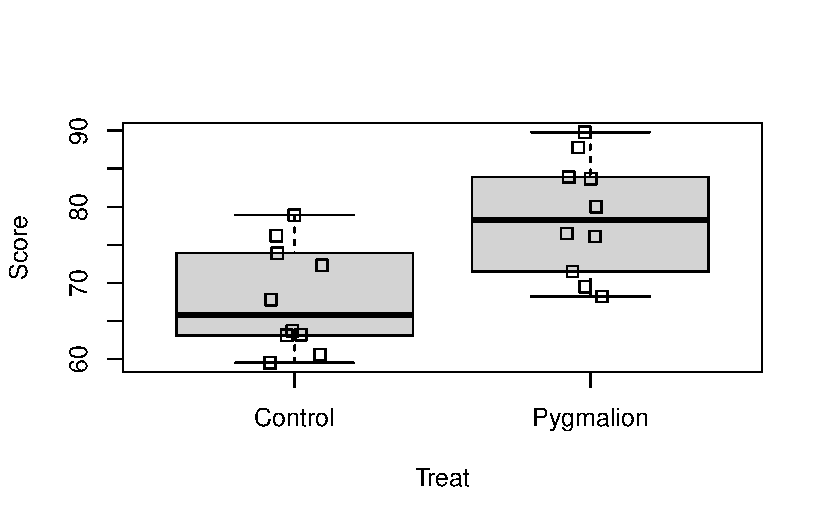
\includegraphics[keepaspectratio]{11_RCBD_Assump_files/figure-pdf/unnamed-chunk-3-1.pdf}}

Okay, the boxplots look relatively symmetric, there are no clear signs
of non-normality. They also look very similar in terms of height, the
assumption of homogeneity seems reasonable as well. Let's have a look at
the sample standard deviations.

\begin{Shaded}
\begin{Highlighting}[]
\FunctionTok{sd}\NormalTok{(pyg\_data}\SpecialCharTok{$}\NormalTok{Score[pyg\_data}\SpecialCharTok{$}\NormalTok{Treat }\SpecialCharTok{==} \StringTok{"Pygmalion"}\NormalTok{])}
\end{Highlighting}
\end{Shaded}

\begin{verbatim}
[1] 7.587124
\end{verbatim}

\begin{Shaded}
\begin{Highlighting}[]
\FunctionTok{sd}\NormalTok{(pyg\_data}\SpecialCharTok{$}\NormalTok{Score[pyg\_data}\SpecialCharTok{$}\NormalTok{Treat }\SpecialCharTok{==} \StringTok{"Control"}\NormalTok{])}
\end{Highlighting}
\end{Shaded}

\begin{verbatim}
[1] 6.927209
\end{verbatim}

Then, we need to check the independence assumption. This is often the
hardest assumption to verify because it requires knowledge about how the
data were collected. In practice, you will need to assess independence
in one of two ways:

\begin{enumerate}
\def\labelenumi{\arabic{enumi}.}
\tightlist
\item
  Before conducting an experiment -- Ideally, you would discuss the
  study design with the researchers before data collection to ensure
  that independence is maintained.
\item
  When analyzing existing data -- If you are reviewing a published
  study, you must rely on the authors' description of the experimental
  setup to determine whether independence is reasonable.
\end{enumerate}

In this study, the researchers assumed platoons operated independently
and took steps to prevent treatment contamination:

\begin{itemize}
\tightlist
\item
  Randomization ensured that each platoon was independently assigned to
  the Pygmalion or control condition, reducing bias.
\item
  Leaders were instructed not to discuss their treatment condition,
  preventing expectation spillover.
\item
  Each platoon was analyzed separately, ensuring observations within
  treatments were treated as independent.
\end{itemize}

After fitting the model, and assuming the order in which the response
was measured is the order in which it appears in the data set, we can
check for any pattern in the residuals that may indicate dependence.

Now, let's check the new assumption of additivity. We can plot the
response against treatment and add colour-coded lines connecting the
experimental units from the same block. This is a bit tedious to do with
base R (don't worry, we won't expect you to code this manually) but you
have to understand and interpret the plot it produces.

\begin{Shaded}
\begin{Highlighting}[]
\CommentTok{\# Ensure Treat is a factor with proper order}
\NormalTok{pyg\_data}\SpecialCharTok{$}\NormalTok{Treat }\OtherTok{\textless{}{-}} \FunctionTok{factor}\NormalTok{(pyg\_data}\SpecialCharTok{$}\NormalTok{Treat, }\AttributeTok{levels =} \FunctionTok{c}\NormalTok{(}\StringTok{"Control"}\NormalTok{, }\StringTok{"Pygmalion"}\NormalTok{))}

\CommentTok{\# Convert Treat to numeric for plotting (1 = Control, 2 = Pygmalion)}
\NormalTok{pyg\_data}\SpecialCharTok{$}\NormalTok{Treat\_numeric }\OtherTok{\textless{}{-}} \FunctionTok{as.numeric}\NormalTok{(pyg\_data}\SpecialCharTok{$}\NormalTok{Treat)}

\CommentTok{\# Define colors for companies}
\NormalTok{company\_colors }\OtherTok{\textless{}{-}} \FunctionTok{rainbow}\NormalTok{(}\FunctionTok{length}\NormalTok{(}\FunctionTok{unique}\NormalTok{(pyg\_data}\SpecialCharTok{$}\NormalTok{Company)))}
\FunctionTok{names}\NormalTok{(company\_colors) }\OtherTok{\textless{}{-}} \FunctionTok{unique}\NormalTok{(pyg\_data}\SpecialCharTok{$}\NormalTok{Company)}

\CommentTok{\# Create base plot}
\FunctionTok{plot}\NormalTok{(pyg\_data}\SpecialCharTok{$}\NormalTok{Treat\_numeric, pyg\_data}\SpecialCharTok{$}\NormalTok{Score, }
     \AttributeTok{xlab =} \StringTok{"Treatment"}\NormalTok{, }\AttributeTok{ylab =} \StringTok{"Score"}\NormalTok{, }
     \AttributeTok{main =} \StringTok{"Pygmalion Effect by Company"}\NormalTok{,}
     \AttributeTok{pch =} \DecValTok{16}\NormalTok{, }\AttributeTok{col =}\NormalTok{ company\_colors[pyg\_data}\SpecialCharTok{$}\NormalTok{Company], }\AttributeTok{xaxt =} \StringTok{"n"}\NormalTok{)}

\CommentTok{\# Add custom x{-}axis labels}
\FunctionTok{axis}\NormalTok{(}\DecValTok{1}\NormalTok{, }\AttributeTok{at =} \FunctionTok{c}\NormalTok{(}\DecValTok{1}\NormalTok{, }\DecValTok{2}\NormalTok{), }\AttributeTok{labels =} \FunctionTok{c}\NormalTok{(}\StringTok{"Control"}\NormalTok{, }\StringTok{"Pygmalion"}\NormalTok{))}

\CommentTok{\# Add lines connecting observations from the same company}
\ControlFlowTok{for}\NormalTok{(block }\ControlFlowTok{in} \FunctionTok{unique}\NormalTok{(pyg\_data}\SpecialCharTok{$}\NormalTok{Company))\{}
\NormalTok{  temp }\OtherTok{\textless{}{-}}\NormalTok{ pyg\_data[pyg\_data}\SpecialCharTok{$}\NormalTok{Company }\SpecialCharTok{==}\NormalTok{ block, ]}
\NormalTok{  temp }\OtherTok{\textless{}{-}}\NormalTok{ temp[}\FunctionTok{order}\NormalTok{(temp}\SpecialCharTok{$}\NormalTok{Treat\_numeric), ]  }\CommentTok{\# Order by treatment for correct line drawing}
  \FunctionTok{lines}\NormalTok{(temp}\SpecialCharTok{$}\NormalTok{Treat\_numeric, temp}\SpecialCharTok{$}\NormalTok{Score, }\AttributeTok{col =}\NormalTok{ company\_colors[block], }\AttributeTok{lwd =} \DecValTok{2}\NormalTok{)}
\NormalTok{\}}
\end{Highlighting}
\end{Shaded}

\pandocbounded{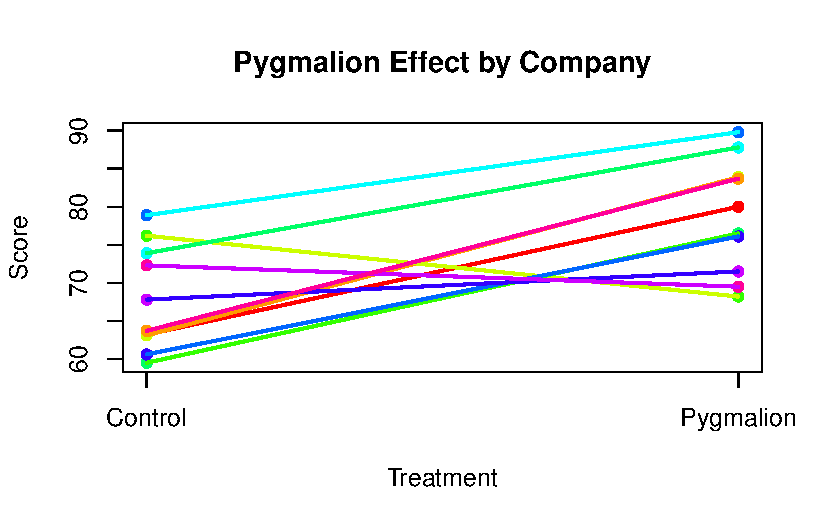
\includegraphics[keepaspectratio]{11_RCBD_Assump_files/figure-pdf/unnamed-chunk-5-1.pdf}}

If the assumption of additivity is met, we would expect relatively few
lines to cross, i.e.~we would expect mostly parallel lines. In the plot
above, it seems that for most blocks, a low value in the control
treatment is associated with a high value in the Pygmalion treatment.
There are three lines (i.e.~companies) that don't conform to this
pattern, where it seems that Pygmalion treatment did not alter the
scores or maybe even caused a reduction. It's important to remember that
\textbf{sampling variability} prevents us from observing perfectly
parallel lines in practice. The observed treatment means are always
subject to \textbf{random variation}, which can introduce some
deviations from the expected pattern.

What happens if this assumption is wrong, i.e.~the blocking and
treatment factors do interact? That is the treatment effect depends on
which block it is in. Consider the following plots depicting an
experiment with three treatments and three blocks. The first panel shows
an example where treatments and blocks are additive -- the lines
connecting the same treatment in all blocks are parallel. Due to
variability, we would of course never actually observe such parallel
lines. In reality, the observed treatment means would be subject to
random deviations from the true population means, and with lots of
variability, the lines could cross and look more like the second panel,
which is showing an example where the additivity assumption is violated.

\pandocbounded{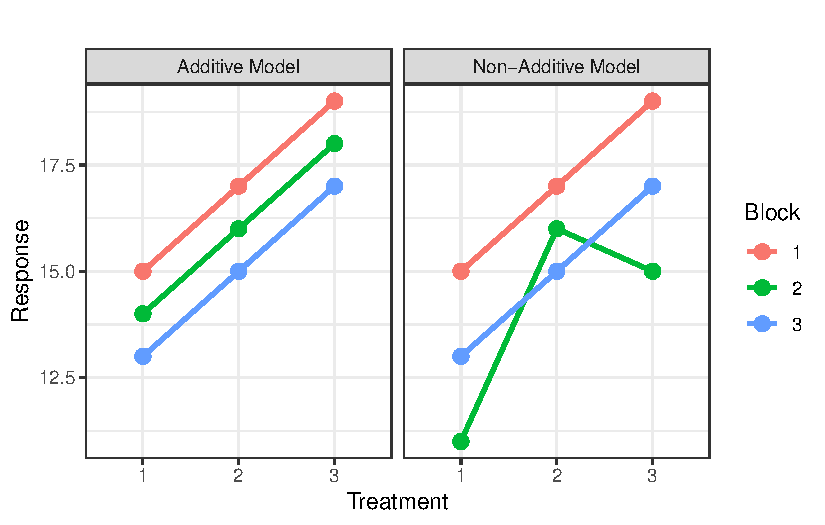
\includegraphics[keepaspectratio]{11_RCBD_Assump_files/figure-pdf/unnamed-chunk-6-1.pdf}}

With only one experimental unit per treatment in each block, as in a
typical randomised complete block design, it is difficult to know which
situation we have: the additivity assumption is violated, or there is
simply a lot of random error. The interaction effect between treatment
and block is confounded with the random error term. That is, \(e_{ij}\)
in the model equation is actually the sum of the interaction effect and
the random error. So if the additivity assumption is violated,
\(e_{ij}\) is inflated and it will be harder to find differences between
treatments.

\marginnote{\begin{footnotesize}

With some replication of treatments within blocks, as in generalised
randomised complete block designs (which we don't cover here), we can
separately estimate the interaction effects. This is similar to what we
will see when we talk about Factorial Experiment sin the next section.

\end{footnotesize}}

\chapter{Linear model \& ANOVA}\label{linear-model-anova}

\section*{Linear model}\label{linear-model}
\addcontentsline{toc}{section}{Linear model}

\markright{Linear model}

We wish to compare \(a\) treatments and have \(N\) experimental units
arranged in \(b\) blocks each containing \(a\) homogeneous experimental
units: \(N = ab\). The \(a\) treatments are assigned to the units in the
\(j^{th}\) block at random. The design (blocking and treatment factors
and the randomisation) determine the structural part of the model.

A linear model for the RBD is:

\[Y_{ij} = \mu + A_i + B_j  +e_{ij}\]

where,

\[
\begin{aligned}
    Y_{ij} &= \text{observation on treatment } i \text{ in block } j \\
    i &= 1, \dots, a \text{ and } j = 1, \dots, b \\
    \mu &= \text{general/overall mean} \\
    A_i &= \text{effect of the } i^{th} \text{ treatment} \\
    B_j &= \text{effect of the } j^{th} \text{ block} \\
    e_{ij} &= \text{random error with } e_{ij} \sim N(0, \sigma^2) \\
    \sum_{i=1}^{a} A_i &= \sum_{j=1}^{b} B_j = 0
\end{aligned}
\]

This model says that each observation is made up of an overall mean, a
treatment effect, a block effect, and an error part. The block effect is
interpreted in the same way as the treatment effect, it is the
difference between block mean \(j\) and the overall mean \(\mu\).

It also says that these effects are additive. Additivity means that the
effect of the \(i^{th}\) treatment on the response (\(A_i\)) is the same
regardless of the block in which the treatment is used. Similarly, the
effect of the \(j^{th}\) block is the same (\(B_j\)) regardless of the
treatment. The additional constraint of \(\sum_{j=1}^{b} \beta_j = 0\)
follows the same logic as explained before.

Let's fit this model to the Pygmalion data. For the Pygmalion
experiment, the researchers compared control to Pygmalion treatment so
we have \(a=2\) treatments. The number of blocks, \(b\), was 10. In R,
on the right-hand-side of the formula, we have the treatment factor +
blocking factor. The code looks exactly the same as before, except we
\textbf{add} the Company (blocking) variable.

\begin{Shaded}
\begin{Highlighting}[]
\NormalTok{pyg\_model }\OtherTok{\textless{}{-}} \FunctionTok{aov}\NormalTok{(Score }\SpecialCharTok{\textasciitilde{}}\NormalTok{ Treat }\SpecialCharTok{+}\NormalTok{ Company, }\AttributeTok{data =}\NormalTok{ pyg\_data)}
\end{Highlighting}
\end{Shaded}

We can again extract the model estimates with \texttt{model.table}:

\begin{Shaded}
\begin{Highlighting}[]
\FunctionTok{model.tables}\NormalTok{(pyg\_model, }\AttributeTok{type =} \StringTok{"means"}\NormalTok{, }\AttributeTok{se =} \ConstantTok{TRUE}\NormalTok{)}
\end{Highlighting}
\end{Shaded}

\begin{verbatim}
Tables of means
Grand mean
      
73.31 

 Treat 
Treat
  Control Pygmalion 
    67.92     78.70 

 Company 
Company
   C1   C10    C2    C3    C4    C5    C6    C7    C8    C9 
71.60 73.70 73.50 72.20 68.00 80.85 84.35 68.35 69.65 70.90 

Standard errors for differences of means
        Treat Company
        3.126   6.990
replic.    10       2
\end{verbatim}

First we see the grand mean of 73.31 followed by the treatment means.
Then, we have ten block means, these are the mean scores within each
block. Lastly, we see the standard errors for the differences of means.

\section*{Sums of squares and Analysis of
variance}\label{sums-of-squares-and-analysis-of-variance}
\addcontentsline{toc}{section}{Sums of squares and Analysis of variance}

\markright{Sums of squares and Analysis of variance}

Now we have three sources of variability: differences between
treatments, differences between blocks and experimental error. The total
sum of squares can be split into three sums of squares: for treatments,
blocks, and error respectively.

\[
SS_{total} = SS_A + SS_B + SSE
\]

with degrees of freedom

\[
(ab - 1) = (a - 1) + (b - 1) + (a - 1)(b - 1)
\]

The advantage of blocking becomes apparent here. If we had not blocked,
i.e.~used a completely randomised design, for example, the \(SS_A\)
(sums of squares for treatment) would be the same. However, in the
completely randomised design, we would not be able to separate \(SS_B\)
from \(SSE\) and the combined \(SSE\) would therefore be larger.

When using a RBD, part of the unexplained variation is now explained and
can be captured in the block sum of squares, \(SS_B\). A small \(SSE\)
has the advantage of smaller standard errors, i.e.~more precise
estimates (for treatment effects and treatment means) and thus it is
easier to detect differences between treatments.

\marginnote{\begin{footnotesize}

You can think of the SSE as the variability among experimental units
that cannot be accounted for by blocks or treatments.

\end{footnotesize}}

The sums of squares are summarised in an ANOVA table.

\begin{longtable}[]{@{}
  >{\raggedright\arraybackslash}p{(\linewidth - 8\tabcolsep) * \real{0.2000}}
  >{\raggedright\arraybackslash}p{(\linewidth - 8\tabcolsep) * \real{0.2000}}
  >{\raggedright\arraybackslash}p{(\linewidth - 8\tabcolsep) * \real{0.2000}}
  >{\raggedright\arraybackslash}p{(\linewidth - 8\tabcolsep) * \real{0.2000}}
  >{\raggedright\arraybackslash}p{(\linewidth - 8\tabcolsep) * \real{0.2000}}@{}}
\toprule\noalign{}
\begin{minipage}[b]{\linewidth}\raggedright
Source
\end{minipage} & \begin{minipage}[b]{\linewidth}\raggedright
SS
\end{minipage} & \begin{minipage}[b]{\linewidth}\raggedright
df
\end{minipage} & \begin{minipage}[b]{\linewidth}\raggedright
MS
\end{minipage} & \begin{minipage}[b]{\linewidth}\raggedright
F
\end{minipage} \\
\midrule\noalign{}
\endhead
\bottomrule\noalign{}
\endlastfoot
Treatments A & \(SS_A = b \sum_i (\bar{Y}_i - \bar{Y}_{..})^2\) &
\((a - 1)\) & \(\frac{SS_A}{(a-1)}\) & \(\frac{MS_A}{MSE}\) \\
Blocks B & \(SS_B = a \sum_j (\bar{Y}_j - \bar{Y}_{..})^2\) &
\((b - 1)\) & \(\frac{SS_B}{(b-1)}\) & \\
Error &
\(SSE = \sum_{ij} (Y_{ij} - \bar{Y}_{i.} - \bar{Y}_{.j} + \bar{Y}_{..})^2\)
& \((a - 1)(b - 1)\) & \(\frac{SSE}{(a-1)(b-1)}\) & \\
Total & \(SS_{total} = \sum (Y_{ij} - \bar{Y}_{..})^2\) & \(ab - 1\) &
& \\
\end{longtable}

Much of the table remains the same as in a one-way ANOVA, but now it
includes an additional row for the blocking variable. The sum of squares
for the blocking factor is calculated similarly to that of the treatment
factor---by summing the squared deviations of observations within each
block from the block's mean response. The residual sum of squares is
also slightly different, but you don't need to worry too much about
that\footnote{You can easily get there by rearranging the model equation
  so that \(e_{ij}\) is on the right-hand-side, replacing the effects
  with the difference in terms of means and simplifying.}. Since the
total SS is simply the sum of the treatment, block, and residual SS, you
can always compute SSE by subtraction.

From this ANOVA table, we can test the hypothesis of no differences
between the treatment means as before.

\[H_0: \mu_! = \mu_2 = \ldots =\mu_a\]

Which is equivalent to testing:

\[
H_0 : \alpha_1 = \alpha_2 = \dots = \alpha_a = 0
\]

using the F-test which compares the mean square for treatments with the
mean square for error:

\[
F = \frac{MS_A}{MSE} \sim F_{a-1, (a-1)(b-1)}
\]

Notice the degrees of freedom!

What does the ANOVA table look like for the Pygmalion data? Again, we
use the \texttt{summary} function on the model object to obtain the
table.

\begin{Shaded}
\begin{Highlighting}[]
\FunctionTok{summary}\NormalTok{(pyg\_model)}
\end{Highlighting}
\end{Shaded}

\begin{verbatim}
            Df Sum Sq Mean Sq F value  Pr(>F)   
Treat        1  581.0   581.0   11.89 0.00729 **
Company      9  510.2    56.7    1.16 0.41433   
Residuals    9  439.8    48.9                   
---
Signif. codes:  0 '***' 0.001 '**' 0.01 '*' 0.05 '.' 0.1 ' ' 1
\end{verbatim}

Let's first look at the degrees of freedom:

\begin{itemize}
\tightlist
\item
  We had \(a \times b = 2 \times 10 = 20\) experimental units, so we
  should have \(a \times b - 1\) total degrees of freedom.
\item
  The treatment degrees of freedom are \(a-1 = 2-1 = 1\) and similarity,
  there are \(b-1 = 10 -1=9\) degrees of freedom of the block effect.
\item
  That leaves \((a-1)(b-1) = 1 \times 9\) degrees of freedom for the
  error term.
\end{itemize}

It is always a good idea to check that the df's match with what you
expected them to be. One serious error that happens easily is one of the
factor is fitted as continuous covariate because the levels were
labelled using numbers. Hence why we converted the categorical variables
(Treat and Company) to factors.

The next column lists the sums of squares for the three components. The
mean squares are calculated as \(\frac{SS}{df}\),
e.g.~\(\frac{581}{1} = 581\) for the treatment. The \(F\)-value for the
treatment variable is the ratio of \(MS_{treat}\) to the \(MSE\). This
is the same as in the one-way ANOVA. R then looks up the corresponding
p-value, which is \(0.00729\).

So we have an very small p-value which means that we have strong
evidence against our null hypothesis of equal treatment means. We cannot
conclude that the effects are equal to zero. There is evidence to
suggest that at least one treatment resulted in a different mean score.
Here, because we have two treatments, the results indicate that the data
are not compatible with a null hypothesis of equal means. We make the
following conclusion:

``There is evidence to suggest that the two treatment means are
different (\(F = 11.89\), \(p = 0.0073\)).''

If we had more than two treatment means as is usually the case, we would
conclude:

``There is evidence to suggest that at least one treatment resulted in a
different mean response, there is evidence for a treatment effect
(\(F = 11.89\), \(p = 0.0073\)).''

There are many different ways to say that there is a difference
somewhere. For example:

\begin{itemize}
\tightlist
\item
  One or more treatments had a mean response that differed from the
  others.
\item
  Not all treatment means are the same; at least one is significantly
  different.
\item
  The results indicate that not all treatment means are equal.
\end{itemize}

You get the idea! As long as it is clear that a `significant' result
indicates that there is a difference somewhere, we don't know where, but
there is evidence for a treatment effect.

\section*{What about the F-test for the blocking
variable?}\label{what-about-the-f-test-for-the-blocking-variable}
\addcontentsline{toc}{section}{What about the F-test for the blocking
variable?}

\markright{What about the F-test for the blocking variable?}

We see that the blocks accounted for a similar fraction of the sums of
squares as the other two components (just over a third). If we did not
block, this variation would be part of the SSE but then the error
degrees of freedom would also be larger (the 9 degrees of freedom would
be part of the error degrees of freedom). In fact, here, the blocking
did not significantly reduce the unexplained variability, since the
F-value is close to one. The variability explained by the blocks is
close to what would be expected due to random noise.

Remember, we aren't particularity interested in formal inference about
block effects (we knew or suspected that they were different) and we
should always be careful about interpreting the F-test for the blocking
variable (as blocks typically cannot be randomised to experimental units
- see the previous chapter). We might, however, be interested in whether
blocking increased the efficiency of the design by reducing the
unexplained variation (SSE). There exists a more thorough method of
assessing the relative efficiency of blocking - that is, relative to if
a simpler design (i.e.~CRD) was used instead\footnote{Kuehl
  (\citeproc{ref-kuehl2000design}{2000}) wrote a great textbook (freely
  available) that explains the relative efficiency check in detail.}.
Here, however, we focus on a simple and quick check of block efficiency
using the F-ratio.

We would like the block factor to explain a lot of variation. If the
mean square of the blocking variable is larger than the error mean
square we conclude that blocking was effective (compared to a CRD).

\begin{itemize}
\item
  If \(F > 1\) then blocking did reduce unexplained error variance.
\item
  If \(F \approx 1\) then the blocks did not improve the power of the
  experiment and you would have been equally well off with a CRD.
\item
  If \(F<1\) which happens rarely, it means that blocking did not
  account for much of the variability because experimental units within
  blocks are more heterogeneous than between blocks (or there are strong
  interactions between blocks and treatments). Blocks actually reduced
  the power of the experiment but this should really not happen if you
  choose your blocks sensibly.
\end{itemize}

If blocking was not efficient, we would still leave the block factor in
the model (\textbf{design dictates analysis}), but we might decide not
to use blocking in a similar experiment in the future because it didn't
assist in reducing experimental error variance and only cost us degrees
of freedom.

\section*{Estimation}\label{estimation-1}
\addcontentsline{toc}{section}{Estimation}

\markright{Estimation}

To obtain estimates for the treatment and block effects, we minimize the
error sum of squares (method of least squares).

\[
SSE = \sum_i \sum_j (Y_{ij} - \mu - A_i - B_j)^2
\]

\(Y_{ij} - \mu - \alpha_i - \beta_j\) is the observed value minus the
expected value (the structural part of the model). This difference is
just the error \(e_{ij}\). If we minimise the error sum of squares we
obtain the following estimates:

\[
\hat{\mu} = \bar{Y}_{..}
\]

\[
\hat{A_i} = \bar{Y}_{i.} - \bar{Y}_{..}, \quad i = 1 \dots a
\]

\[
\hat{B_j} = \bar{Y}_{.j} - \bar{Y}_{..}, \quad j = 1 \dots b
\]

To estimate the \(i^{th}\) treatment effect we take the observed
treatment mean minus the overall mean, similarly to obtain block effect
estimates.

\chapter{Contrasts}\label{contrasts-1}

After finding that there is evidence to suggest that at least two of the
treatments differed from each other (another way to say there is a
treatment effect!), we want to find out which ones differed and estimate
these differences. In the Pygmalion experiment, there were only two
treatments so we know the difference is between them. In fact, we could
have used a paired t-test to analyse the data and we would get the same
results. Generally though, there will be more than two treatments and
then after concluding that there are differences, we want to know where
the differences lie.

\marginnote{\begin{footnotesize}

When we have blocks in RCBD, the observations are paired and data from
two treatments can be analysed using a paired t-test. When we do not
have blocks, the observations are not and data from two treatments can
be analysed using a standard t-test.

\end{footnotesize}}

To do that, we use the coefficients from fitting a linear regression
model to estimate the difference between the two treatments (as we did
for CRD experiments as well). The null hypothesis is again:

\[H_0: \mu_C - \mu_P = 0 \]

where C stands for Control and P for Pygmalion. We use the \texttt{lm}
function as in regression.

\marginnote{\begin{footnotesize}

We use the \texttt{lm} function when we are primarily interested in the
coefficient estimates and difference. We use \texttt{aov()} when we want
a breakdown of how much each factor can explain of the overall variation
in the response, and when we want a general test for `are there
\emph{any} difference between the treatments'.

\end{footnotesize}}

\begin{Shaded}
\begin{Highlighting}[]
\NormalTok{pyg\_model\_reg }\OtherTok{\textless{}{-}} \FunctionTok{lm}\NormalTok{(Score }\SpecialCharTok{\textasciitilde{}}\NormalTok{ Treat }\SpecialCharTok{+}\NormalTok{ Company, }\AttributeTok{data =}\NormalTok{ pyg\_data)}
\FunctionTok{summary}\NormalTok{(pyg\_model\_reg)}
\end{Highlighting}
\end{Shaded}

\begin{verbatim}

Call:
lm(formula = Score ~ Treat + Company, data = pyg_data)

Residuals:
   Min     1Q Median     3Q    Max 
-9.390 -3.217  0.000  3.217  9.390 

Coefficients:
               Estimate Std. Error t value Pr(>|t|)    
(Intercept)      66.210      5.184  12.771 4.52e-07 ***
TreatPygmalion   10.780      3.126   3.448  0.00729 ** 
CompanyC10        2.100      6.990   0.300  0.77069    
CompanyC2         1.900      6.990   0.272  0.79191    
CompanyC3         0.600      6.990   0.086  0.93348    
CompanyC4        -3.600      6.990  -0.515  0.61897    
CompanyC5         9.250      6.990   1.323  0.21839    
CompanyC6        12.750      6.990   1.824  0.10147    
CompanyC7        -3.250      6.990  -0.465  0.65303    
CompanyC8        -1.950      6.990  -0.279  0.78659    
CompanyC9        -0.700      6.990  -0.100  0.92243    
---
Signif. codes:  0 '***' 0.001 '**' 0.01 '*' 0.05 '.' 0.1 ' ' 1

Residual standard error: 6.99 on 9 degrees of freedom
Multiple R-squared:  0.7127,    Adjusted R-squared:  0.3936 
F-statistic: 2.233 on 10 and 9 DF,  p-value: 0.1211
\end{verbatim}

A few things to note here.

\begin{enumerate}
\def\labelenumi{\arabic{enumi}.}
\item
  We are only interested in the second line starting with
  \texttt{TreatPygmalion}. R pasted the name of the factor and the name
  of the treatment level together.
\item
  The Control treatment was taken as the baseline (it comes first in the
  alphabet).
\item
  The remaining lines are not of interest to us. It estimates the
  differences between each block and the first and tests whether these
  effects are different from zero. R doesn't know we aren't interested
  in these, so it computes the effects and hypothesis test as if we are.
  We ignore this part.
\item
  If we didn't know that this code was for analysing a RCBD we would
  probably think that it is linear regression with two categorical
  variables. Think back to the regression module, what does this
  intercept represent? It represents the mean score for some treatment
  level and company. Since `C' comes before `P' in the alphabet and C1
  is before everything else, the intercept is the average score for the
  control group in the first block. This is because R uses the
  \emph{treatment contrast} parameterisation by default for all the
  factors. We can change this by letting R know that the block effects
  sum to zero.
\end{enumerate}

\begin{Shaded}
\begin{Highlighting}[]
\NormalTok{pyg\_model\_reg2 }\OtherTok{\textless{}{-}} \FunctionTok{lm}\NormalTok{(Score }\SpecialCharTok{\textasciitilde{}}\NormalTok{ Treat }\SpecialCharTok{+} \FunctionTok{C}\NormalTok{(}\FunctionTok{as.factor}\NormalTok{(Company), contr.sum), }\AttributeTok{data =}\NormalTok{ pyg\_data)}
\FunctionTok{summary}\NormalTok{(pyg\_model\_reg2)}
\end{Highlighting}
\end{Shaded}

\begin{verbatim}

Call:
lm(formula = Score ~ Treat + C(as.factor(Company), contr.sum), 
    data = pyg_data)

Residuals:
   Min     1Q Median     3Q    Max 
-9.390 -3.217  0.000  3.217  9.390 

Coefficients:
                                  Estimate Std. Error t value Pr(>|t|)    
(Intercept)                         67.920      2.211  30.725 2.01e-10 ***
TreatPygmalion                      10.780      3.126   3.448  0.00729 ** 
C(as.factor(Company), contr.sum)1   -1.710      4.689  -0.365  0.72379    
C(as.factor(Company), contr.sum)2    0.390      4.689   0.083  0.93554    
C(as.factor(Company), contr.sum)3    0.190      4.689   0.041  0.96857    
C(as.factor(Company), contr.sum)4   -1.110      4.689  -0.237  0.81818    
C(as.factor(Company), contr.sum)5   -5.310      4.689  -1.132  0.28675    
C(as.factor(Company), contr.sum)6    7.540      4.689   1.608  0.14232    
C(as.factor(Company), contr.sum)7   11.040      4.689   2.354  0.04300 *  
C(as.factor(Company), contr.sum)8   -4.960      4.689  -1.058  0.31775    
C(as.factor(Company), contr.sum)9   -3.660      4.689  -0.780  0.45514    
---
Signif. codes:  0 '***' 0.001 '**' 0.01 '*' 0.05 '.' 0.1 ' ' 1

Residual standard error: 6.99 on 9 degrees of freedom
Multiple R-squared:  0.7127,    Adjusted R-squared:  0.3936 
F-statistic: 2.233 on 10 and 9 DF,  p-value: 0.1211
\end{verbatim}

Now, the intercept is what we expect, the mean score for the control
treatment across all blocks.

\begin{Shaded}
\begin{Highlighting}[]
\FunctionTok{mean}\NormalTok{(pyg\_data}\SpecialCharTok{$}\NormalTok{Score[pyg\_data}\SpecialCharTok{$}\NormalTok{Treat }\SpecialCharTok{==} \StringTok{"Control"}\NormalTok{])}
\end{Highlighting}
\end{Shaded}

\begin{verbatim}
[1] 67.92
\end{verbatim}

Let's interpret the hypothesis test for the difference between the
treatment means. The estimated difference is 10.78 with a standard error
of 3.126. The test statistic is 3.448 which has a p-value of 0.00729.
Look familiar? It's the exact same p-value we found in the ANOVA table!
That is because the ANOVA is an extension of the t-test to more than two
groups and when we only have two treatments, they are equivalent. In
fact, the test statistics have the following relationship:

\[ t^2 = F\]

Test the result to confirm that it holds. Now, let's return to the
interpretation. The test shows that the difference between the control
and Pygmalion treatment is statistically significant, as indicated by
the extremely small p-value. This provides strong evidence against the
null hypothesis of equal means.

To recall the experiment's design: The researchers aimed to test the
Pygmalion effect while eliminating interpersonal contrasts by assigning
treatments to entire groups. Specifically, platoons within companies
were used as treatment units, and since there were 10 companies, each
with 2 platoons, companies served as blocks. The response variable,
theoretical specialty knowledge, was measured through test scores.

The results of a two-way ANOVA provide evidence of a treatment effect
(\(F = 11.89\), \(p = 0.0073\)). More precisely, the estimated
difference between the control and Pygmalion treatment was 10.78 (s.e. =
\(3.13\), \(t = 3.45\), \(p = 0.0073\)). This suggests that the
Pygmalion effect was successful, as soldiers in the Pygmalion group
scored higher on average than those in the control group.

\marginnote{\begin{footnotesize}

In an actual analysis, we would not report both the ANOVA and t-test
since they are equivalent when we have two treatments.

\end{footnotesize}}

Nice! We're done. Before we move on, I'll summarise the results of the
actual study. The researcher had four different responses:

\begin{itemize}
\tightlist
\item
  Theoretical specialty knowledge (taught by platoon leaders)
\item
  Practical specialty skills (taught by platoon leaders)
\item
  Physical fitness (assessed independently)
\item
  Target shooting (assessed independently)
\end{itemize}

Significant treatment effects were found for theoretical and practical
specialty scores (\(F = 13.74\), \(p < 0.01\) and \(F = 6.37\),
\(p < 0.05\), respectively). No significant difference was found for
physical fitness or target shooting, confirming that the Pygmalion
effect was specific to areas influenced by leader expectations! This
suggests that high expectations from others can enhance performance,
particularly in areas where they have direct influence. With this in
mind, I want you to know that \textbf{I believe in your potential to
excel in this course and expect nothing less. ;)} On to the next
section!

\part{Factorial Experiments}

\chapter{Introduction}\label{introduction-2}

So far, we have explored experiments with a \textbf{single treatment
factor}. However, in many cases, analyzing factors one at a time does
not fully explain the behavior of the response variable. This is
particularly true when factors interact, meaning that the effect of one
factor depends on the level or setting of another factor.

A factorial experiment involves more than one treatment factor, allowing
us to study how factors interact. In a complete factorial experiment,
every possible combination of factor levels is tested. The total number
of treatments is the product of the number of levels for each factor. In
other words, each treatment is a combination of one level from each
factor.

\section{Factorial Structure vs.~Experimental
Design}\label{factorial-structure-vs.-experimental-design}

It is important to note that a \textbf{factorial experiment is not a
design by itself}---it is a treatment structure. The underlying design
can be:

\begin{itemize}
\tightlist
\item
  A Completely Randomized Design (CRD)
\item
  A Randomized Complete Block Design (RCBD)
\end{itemize}

In the social media multitasking example, suppose the researchers wanted
to know whether the effect of social media multitasking on academic
performance is mitigated by lecture format? We would ask:

\begin{quote}
\emph{Does the effect of social media multitasking on academic
performance depend on lecture format?}
\end{quote}

The experiment would still follow a Completely Randomized Design (CRD)
but now with two treatment factors instead of one.

Similarly, if we extended the Pygmalion experiment to include an
additional factor, we would have an RCBD with two treatment factors.

\section{Notation and Structure of Factorial
Experiments}\label{notation-and-structure-of-factorial-experiments}

In general, if an experiment has two treatment factors with \(a\) and
\(c\) levels, then there are \(a \times c\) treatments. This is called
an \(a \times c\) factorial treatment structure.

To clarify the terminology:

\begin{itemize}
\tightlist
\item
  A \textbf{treatment factor} has \textbf{different levels} (e.g.,
  social media multitasking: \emph{none, texting, Facebook}).
\item
  \textbf{Treatments} are the \textbf{combinations} of factor levels
  (e.g., \emph{no multitasking + lecture format A}, \emph{texting +
  lecture format B}).
\end{itemize}

In factorial experiments, the treatment factors are said to be
\emph{crossed}, meaning that all levels of one factor appear at all
levels of the other factor.

\section{Randomisation in Factorial
Experiments}\label{randomisation-in-factorial-experiments}

Randomization in factorial experiments depends on the chosen design and
is carried out similarly to single-factor experiments. In R, it is
helpful to number or name the treatments systematically.

Suppose we have two factors:

\begin{itemize}
\tightlist
\item
  Marketing Strategy (2 levels: \(m_0, m_1\))
\item
  Product Promotion (2 levels: \(p_0, p_1\))
\end{itemize}

This creates \textbf{four treatments}:

\(m_0p_0\), \(m_0p_1\), \(m_1p_0\), \(m_1p_1\)

If we have 12 experimental units and no need for blocking, we conduct a
Completely Randomized Design (CRD) as follows:

\begin{Shaded}
\begin{Highlighting}[]
\NormalTok{treats }\OtherTok{\textless{}{-}} \FunctionTok{c}\NormalTok{(}\StringTok{"m0p0"}\NormalTok{, }\StringTok{"m0p1"}\NormalTok{, }\StringTok{"m1p0"}\NormalTok{, }\StringTok{"m1p1"}\NormalTok{)}
\NormalTok{treats }\OtherTok{\textless{}{-}} \FunctionTok{rep}\NormalTok{(treats, }\AttributeTok{each =} \DecValTok{3}\NormalTok{)  }\CommentTok{\# Repeat each treatment 3 times}
\NormalTok{treats }
\end{Highlighting}
\end{Shaded}

\begin{verbatim}
 [1] "m0p0" "m0p0" "m0p0" "m0p1" "m0p1" "m0p1" "m1p0" "m1p0" "m1p0" "m1p1"
[11] "m1p1" "m1p1"
\end{verbatim}

\begin{Shaded}
\begin{Highlighting}[]
\NormalTok{r1 }\OtherTok{\textless{}{-}} \FunctionTok{sample}\NormalTok{(treats)  }\CommentTok{\# Randomly assign treatments}

\FunctionTok{cbind}\NormalTok{(}\DecValTok{1}\SpecialCharTok{:}\DecValTok{12}\NormalTok{, r1)  }\CommentTok{\# Display the assignments}
\end{Highlighting}
\end{Shaded}

\begin{verbatim}
           r1    
 [1,] "1"  "m0p1"
 [2,] "2"  "m1p0"
 [3,] "3"  "m0p0"
 [4,] "4"  "m0p0"
 [5,] "5"  "m0p0"
 [6,] "6"  "m1p1"
 [7,] "7"  "m0p1"
 [8,] "8"  "m1p1"
 [9,] "9"  "m1p1"
[10,] "10" "m1p0"
[11,] "11" "m1p0"
[12,] "12" "m0p1"
\end{verbatim}

This code assigns treatments randomly and prints the experimental unit
number alongside its assigned treatment. If we had blocking, we would
repeat the randomization separately for each block.

\section{Is comprehension affect by playback speed and lecture
modality?}\label{is-comprehension-affect-by-playback-speed-and-lecture-modality}

In keeping with the theme of students, learning and teaching. Have you
ever wondered whether playback speed affects your comprehension of a
lecture? Or whether your comprehension is better with audio-only
lectures such as podcast versus recorded lectures with visuals? What
about if you listen to a podcast at double speed versus a recorded
lecture at double speed, is there difference in comprehension? to answer
this question, researchers from the University of California conducted a
\(2\times2\) factorial experiment.

\begin{tcolorbox}[enhanced jigsaw, opacitybacktitle=0.6, colbacktitle=quarto-callout-warning-color!10!white, toprule=.15mm, bottomtitle=1mm, breakable, leftrule=.75mm, rightrule=.15mm, left=2mm, colback=white, coltitle=black, toptitle=1mm, colframe=quarto-callout-warning-color-frame, bottomrule=.15mm, title={Lecture modality and playback speed}, arc=.35mm, titlerule=0mm, opacityback=0]

Chen et al. (\citeproc{ref-chen2024effect}{2024}) conducted an
experiment to find out whether visual information improves comprehension
when lectures are played at faster speeds. Specifically, they wanted to
investigate the effect of \emph{lecture modality} (audio-only or
audio-visual) and \emph{playback speed} (1x or 2x) on comprehension of
students and whether these factors interact. We can summarise the
research questions as follows:

\begin{enumerate}
\def\labelenumi{\arabic{enumi}.}
\tightlist
\item
  Does lecture modality have an effect on comprehension?
\item
  Does playback speed have an effect on comprehension?
\item
  Is there an interaction effect of modality and playback speed on
  comprehension?
\end{enumerate}

A total of 200 undergraduate students were randomly assigned to one of
four groups:

\begin{enumerate}
\def\labelenumi{\arabic{enumi}.}
\tightlist
\item
  Audio-only at normal speed (1x)
\item
  Audio-visual (with slides) at normal speed (1x)
\item
  Audio-only at double speed (2x)
\item
  Audio-visual (with slides) at double speed (2x)
\end{enumerate}

The researchers chose two lectures: one about about real estate
appraisals and another bout the history of the Roman Empire. The
lectures were either presented as audio-visual clips which consisted of
presentation slides and instructor images, and no subtitles or captions
were provided. All the graphics (maps, figures) in the slides were
static. For lectures presented as audio-only clips, only the
instructor's audio was made available.

Each student was presented both lectures in the modality and speed they
were assigned. Afterwards, they completed a comprehension test
consisting of 25 multiple choice questions on each topic. The average of
the scores was taken as the final measure of comprehension.

\end{tcolorbox}

\marginnote{\begin{footnotesize}

We will be using the actual data collected but we will only be using a
subset of the information they recorded. The authors conducted a
different analysis which incorporates this extra information. We will
not be doing this as the method they used is outside th scope of this
course.

\end{footnotesize}}

Right! Let's begin with identifying the design. It should be clear that
we have two treatment factors: \emph{lecture modality} and
\emph{playback speed} each with the treatment levels. this means that we
have a total of \(2 \times 2 = 4\) treatments which are the combinations
of the treatment levels. They investigated the effect of these factors
on the comprehension of students - that means, comprehension is the
response.

\begin{itemize}
\tightlist
\item
  \textbf{Response Variable:} Comprehension\\
\item
  \textbf{Treatment Factors:} Lecture modality and playback speed\\
\item
  \textbf{Treatment Levels:} Lecture modality: Audio-only or
  Audio-visual; Playback speed: 1x or 2x\\
\item
  \textbf{Treatments:} Audio-only at normal speed (1x); Audio-visual at
  normal speed (1x); Audio-only at double speed (2x); Audio-visual at
  double speed (2x)
\end{itemize}

Each student was assigned to one the treatments indicating that students
were the experimental units. The response was also measured on each
student, they are the observational units as well. Therefore, since we
had 200 students and 4 treatment groups, there was 50 students per
group, the experiment had 50 replicates.

\begin{itemize}
\tightlist
\item
  \textbf{Experimental Unit:} Student (200)\\
\item
  \textbf{Observational Unit:} Student (200)\\
\item
  \textbf{Replicates:} 50 students per group\\
\end{itemize}

Lastly, we need to determine how randomisation was conducted. There is
no indication of any blocking and treatments were randomised to the
whole group of experimental units. So this is a Completely Randomised
Design, specifically it is a \(2\times2\) factorial CRD.

\begin{itemize}
\tightlist
\item
  \textbf{Design Type:} \(2\times2\) factorial Completely Randomized
  Design (CRD)
\end{itemize}

Before we do any further analysis, we need to talk a bit about effects!

\chapter{Interactions}\label{interactions}

Interactions between treatment factors are an important reason for
conducting factorial experiments. If the effect of a factor would always
be the same, no matter which other factors are present, and at what
levels, it would be enough to investigate this factor on its own in a
single-factor experiment. However, many factors interact with other
factors, which means that the effects change, depending on the levels of
the other factors.

Up until now, we have spoken rather loosely about `effects'. But at this
point, we need to define more clearly what we mean by the effect of a
treatment or the effect of an explanatory variable. By the effect of a
treatment, we mean the change in response relative to either a reference
or baseline treatment, or often in experiments, to an overall mean
response.

In regression, the effect of a continuous explanatory variable is
measured by the slope, which is the change in response for a one-unit
increase in the explanatory variable, i.e., relative to one unit less.
The effect of categorical or factor variables in regression is the
change in response relative to a reference category.

In experiments, when using an ANOVA model, the effect of a treatment is
mostly measured as the change in response relative to an overall mean
response.

There are different kinds of effects: \textbf{main effects, interaction
effects, and random effects}.

The \textbf{main effect} of a treatment measures the average change in
response, averaged over all levels of the other factors, relative to the
overall mean. When there is only a single factor in an experiment, we
only have main effects.

If the effect of a factor depends on the level of another factor that is
present, then the two factors interact. The \textbf{interaction effect}
represents the change in response relative to the main effects with a
particular treatment.

If there are multiple factors in an experiment, and the effects of one
factor depend on the level of the other factor, i.e., the two factors
interact, the (average) effects might not give a good idea of changes in
the response, or of how the factors affect the response. In such cases,
we need to study the individual treatments more closely. We look at the
combinations of factor levels with large interaction effects.

The figure below illustrates a number of possible interaction situations
in a \(2 \times 2\) factorial experiment, with treatment factor A having
levels a1 and a2, and factor B having levels b1 and b2. To determine
whether main effects of A are present, we must ask whether the average
response changes when moving from a1 to a2, and similarly for main
effects of B.

To determine whether \textbf{interaction effects} are present, we must
ask whether the change in response when moving from a1 to a2 depends on
the level of B. Main effects and interaction effects can both be present
simultaneously.

Before we do anything, orient yourself. What is represented by each
axis, how is the graph differentiating between treatment factors? In the
figure below, the response is on the y-axis and we have the levels of
treatment factor A on the x-axis, the levels of B are denoted by the
colour of the line.

Let's start with (a). The main effect of A is the average change in
response - averaged over all levels of the other factors. Essentially,
we need to determine what happens to the response when we ignore the
levels of B. To do this, we have to calculate the average of the points
at a1 and separately, at a2. When points in a line are eveny
distributed, the average is the mid-point. If you do this for both
levels of A and connect the dots, you will have drawn a flat horizontal
line. Now, going from a1 to a2, what happens to the response? In other
words, does the average response change? No, there is n change which
means there is no main effect of factor A.

Going through the same motions for factor B, reveals that going from b1
to b2 increases the mean response. There is a main effect of factor B.
What about an interaction effect? We ask: does the effect of A on the
response change when we consider the levels of the other factor? now we
do not avearge over the other factor, we take it into account. Looking
at the plot, if we focus on the red line and go from a1 to a2, nothing
happens to the response. If we focus on the black line, the same
(i.e.~nothing) happens to the response as well. If we reverse this and
focus on the points at a1, going from b1 (red) to b2 (black) increases
the response. At a2, the response increases as well by the same amount.
So nothing changed when we considered the other factors, there is no
interaction.

Now, consider plot (e).

\begin{itemize}
\tightlist
\item
  Averaging the response at a1 and a2 results in a horizontal line
  again. No main effect of factor A.
\item
  Averaging the response at b1 and b2, leads to the same conclusion as
  before. Going from b1 to b2, increases the response. There is a main
  effect of factor B.
\item
  If we focus on the red line (b1), going from a1 to a2 increases the
  response. However, at b2, going from a1 to a2 decreases the response!
  The effect of treatment factor A depends on the level of B, they
  interact with each other.
\end{itemize}

So does this mean that A and B have no effect on the response? No, they
both affect the response, their effects, however, depend on the level of
the other factor present.

Plot (e) demonstrates clearly why sometimes main effects cannot be
understood or interpreted when interactions are present. In such a case,
the interaction plot is very helpful to illustrate the effects. Try
deciding for the other plots whether there are main effects for factor A
and B and whether A and B interact. The answers are given in the figure
caption.

\begin{figure}[H]

{\centering \pandocbounded{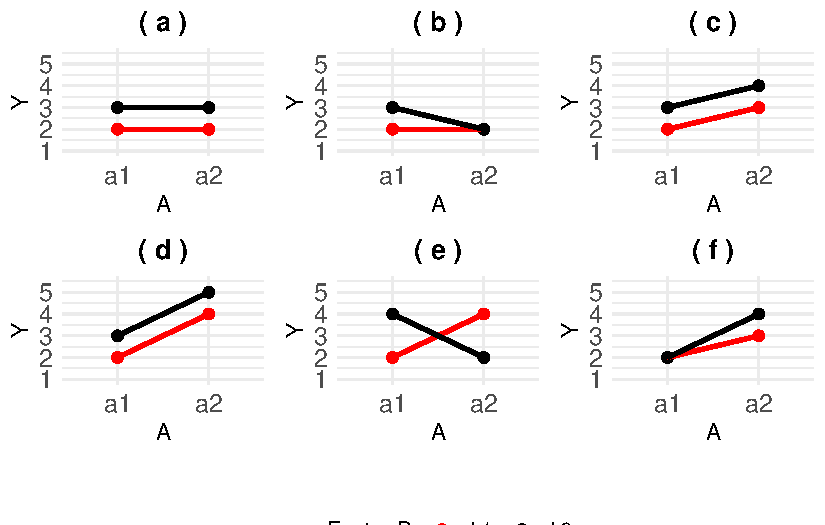
\includegraphics[keepaspectratio]{15_FE_Inter_files/figure-pdf/unnamed-chunk-1-1.pdf}}

}

\caption{Interaction plots for six hypothetical \(2 \times 2\) factorial
experiments. (a) only main effect of B, (b) no main effects and no
interaction effects, (c) only main effect of A, (d) main effect of A and
main effect of B, (e) interaction between A and B, but both main effects
are 0, (f) main effect of B, small main effect of A, A and B interact.}

\end{figure}%

Interaction effects are calculated as the difference between the
treatment mean and the sum of the main effects. To express this more
precisely, it is useful to write down the model.

\section{Can going for a brief walk help with memory
performance?}\label{can-going-for-a-brief-walk-help-with-memory-performance}

We often hear about the benefits of exercise for physical health, but
what about its impact on learning and memory? Would taking a brisk
10-minute walk before studying help us to remember more?

Researchers set out to explore this question by testing whether a short
bout of exercise before learning could enhance memory performance. They
had students either walk or sit before studying a list of words and then
predict how well they would remember them. Later, the students took a
recall test to see how much they actually retained.

Before studying, some students took a 10-minute brisk walk, while others
remained seated and inactive. After this, everyone studied a list of
words and rated how well they thought they would remember them
(Judgements of Learning, or JOLs). Later, they took a free recall test
to see how many words they actually remembered. The researchers wanted
to find out if walking before studying could boost memory and whether
students were aware of any benefits.

\begin{tcolorbox}[enhanced jigsaw, opacitybacktitle=0.6, colbacktitle=quarto-callout-warning-color!10!white, toprule=.15mm, bottomtitle=1mm, breakable, leftrule=.75mm, rightrule=.15mm, left=2mm, colback=white, coltitle=black, toptitle=1mm, colframe=quarto-callout-warning-color-frame, bottomrule=.15mm, title={Warning}, arc=.35mm, titlerule=0mm, opacityback=0]

Salas, Minakata, and Kelemen (\citeproc{ref-walking2011}{2011})
conducted a study to examine whether a brief bout of aerobic exercise
influences memory performance and judgements of learning (JOLs).

A total of 80 college students participated in a 2 × 2 factorial
between-subjects design where they were randomly assigned to one of four
conditions:

Walking-Walking: Participants walked before both encoding and retrieval.
Walking-Sitting: Participants walked before encoding but sat before
retrieval. Sitting-Walking: Participants sat before encoding but walked
before retrieval. Sitting-Sitting (Control): Participants sat before
both encoding and retrieval.

After the activity, all students studied 30 English nouns, provided
immediate JOLs, and then took a free recall test

\end{tcolorbox}

\chapter{Model for Factorial
Experiments}\label{model-for-factorial-experiments}

Assuming we have a continuous response variable for which we assume a
normal distribution, no blocking factors and a factorial experiment with
two treatment factors, the following model is plausible:

\[
Y_{ijk} = \mu + A_i + C_j + (AC)_{ij} + e_{ijk}
\]

where \(Y_{ijk}\) is the \(k^{th}\) observation on the \((ij)^{th}\)
treatment combination and

\[
\begin{aligned}
    Y_{ij} &= \text{observation on treatment } i \text{ in block } j \\
    \mu &= \text{general/overall mean} \\
    A_i &= \text{main effect of the } i^{th} \text{ level of A} \\
    A_i &= \text{main effect of the } j^{th} \text{ level of C} \\
    (AC)_{ij} &= \text{interaction between the }i^{th}\text{ level of A and the }j^{th}\text{ level of C.} \\
    e_{ijk} &= \text{random error with } e_{ijk} \sim N(0, \sigma^2) \\
\end{aligned}
\]

\textbf{Note that (AC) is a single symbol and does not mean the
interpaction is the product of the two main effects.}

\(\mu + A_i + C_j + (AC)_{ij}\) is the structural part of the model
which describes the mean or expected response with treatment \(ij\),
i.e.~at the \(i^{th}\) level of factor A and \(j^{th}\) level of factor
C. Depending on the estimates for the main effects, each treatment will
have a different estimated mean response. For every level of A there is
a main effect, the \(A_i\)'s. For every level of factor B there is a
main effect, \(B_i\). For every combination of A and B levels there is
an interaction effect, \((AC)_{ij}\). So the model implies that each
treatment mean is made up of an overall mean, two main effects and and
interaction term.

\section{Replication}\label{replication-1}

Replication is crucial in any experiment! Without replication, we cannot
estimate the experimental error variance (\(\sigma^2\)), which is
essential for assessing variability and conducting hypothesis tests.

If we only have one observation per treatment, that observation becomes
the treatment mean. Since we cannot compute deviations from the
treatment mean, there is no estimate of error variance. This means that
while we can technically estimate the model parameters, the model itself
is practically useless---we cannot perform hypothesis tests without an
estimate of error variance. And if we can't test anything, what's the
point?

In factorial experiments, the situation gets even worse when we don't
replicate treatments. Specifically, we can't calculate the interaction
effect. In general, the interaction effect is calculated as the
difference between the treatment mean and the sum of the main effects
and the overall mean:

\[(AB)_{ij} = \bar{Y}_{ij} - (\mu + A_i + B_j) \] Now consider the first
plot in the series below. There is only one observation in the
hypothetical treat \(i = 1\) and \(j = 3\). That means that the
treatment mean \(\bar{Y}_{ij}\) is just the mean of this single
observation. We can't calculate any deviations from this mean with only
one observation as we usually would for the error variance. We always
need to calculate an error term and this is always calculated as the
deviation of the observation to the next closest mean. With only one
observation per treatment, the next closest mean to that observation is
the sum of the main effects: \(\mu + A_i + B_j\). But wait, that means
the error term is also the interaction term since the treatment mean and
the observation are the same? Jup! Now you see the problem. With no
replication, the error term and the interaction effect are confounded.

\begin{figure}[H]

{\centering \pandocbounded{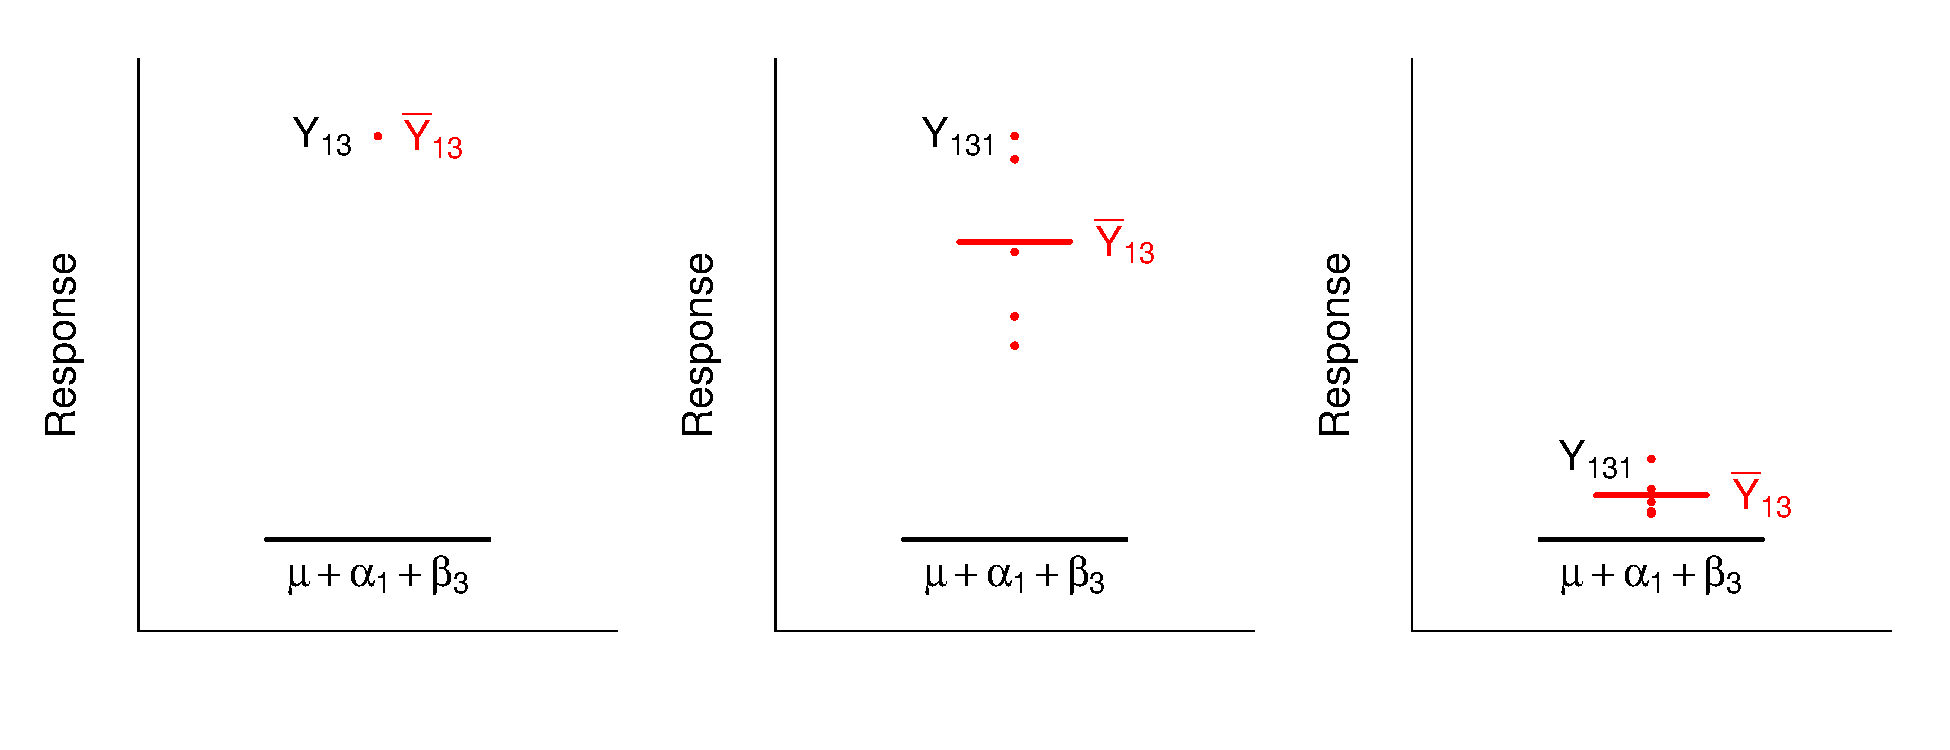
\includegraphics[keepaspectratio]{14_FE_Model_files/figure-pdf/unnamed-chunk-1-1.pdf}}

}

\caption{How is the interaction effect calculated? (a) only one
observation, interaction effect confounded with error term, cannot
estimate interaction effect; (b) large interaction present; (c)
interaction statistically not discernable (very small).}

\end{figure}%

Have a look at the second plot. Now we have five observations within the
treatment. We can calculate the 5 error terms:

\[r_{13k} = Y_{13k} - \bar{Y}_{13}\]

and we can calculate the interaction effect:

\[ (\hat{AB})_{13} = \bar{Y}_{13}- (\hat{\mu} + \hat{A}_1 + \hat{B}_3)\]

They are no longer the same thing, they are separable! The interaction
effect for this treatment is quite big if you look at the difference
visually. For the last plot, there are also five observations, but now
the deviation of the treatment mean from the sum f the main effects is
almost zero; it's just due to random variation. The interaction effect
is too small to detect statistically.

\section{Parameter estimation}\label{parameter-estimation}

The maximum likelihood/least squares estimates are found by minimizing
the error or residual sum of squares:

\[
S = \sum_{ijk} (Y_{ijk} - \mu - \alpha_i - \beta_j - (\alpha\beta)_{ij})^2
\]

The solutions to these equations are the least squares estimates:

\[
\hat{\mu} = \bar{Y}_{...}
\]

\[
\hat{A}_i = \bar{Y}_{i..} - \bar{Y}_{...}, \quad i = 1, \dots, a
\]

\[
\hat{C}_j = \bar{Y}_{.j.} - \bar{Y}_{...}, \quad j = 1, \dots, c
\]

\[
(\hat{AC})_{ij} = \bar{Y}_{ij.} - \bar{Y}_{i..} - \bar{Y}_{.j.} + \bar{Y}_{...}, \quad i = 1, \dots, a, \quad j = 1, \dots,c
\]

The main effects are as before, except that now they refer to
differences between row or column means ({[}Figure 6.3{]}) and the
overall mean. The interaction effects are estimated as the differences
between treatment means and the sum of the main effects.

\section{Back to the example}\label{back-to-the-example}

Let's fit this model to the data of the playback and lecture modality
experiment. This time, we have access to the actual data collected!
Let's explore the data and check our assumptions. The assumptions are
the same as in a one-way ANOVA. That is normality of errors, equal
population variances, independent errors and no outliers.

As always we start by reading in our data, checking that it has been
read in correctly and looking at some descriptive statistics.

\begin{Shaded}
\begin{Highlighting}[]
\NormalTok{data }\OtherTok{\textless{}{-}} \FunctionTok{read.csv}\NormalTok{(}\StringTok{"Datasets/Exp2DataPlayback.csv"}\NormalTok{)}

\FunctionTok{head}\NormalTok{(data)}
\end{Highlighting}
\end{Shaded}

\begin{verbatim}
  Participant.ID       Condition Speed Content.Type Accuracy
1     945445adf5 1x Audio-Visual     2 Audio-Visual       42
2     23afb88ef3        1x Audio     1   Audio-Only       56
3     1bc24e0480        1x Audio     1   Audio-Only       62
4     4fbdbd41a5        1x Audio     1   Audio-Only       44
5     442adf227a        1x Audio     1   Audio-Only       56
6     3ca9d09e2e 1x Audio-Visual     2 Audio-Visual       48
\end{verbatim}

The data set contains 5 columns:

\begin{enumerate}
\def\labelenumi{\arabic{enumi}.}
\tightlist
\item
  \texttt{Participant.ID} -- This column contains a unique
  identification code for each participant in the study.\\
\item
  \texttt{Condition} -- Indicates the experimental condition or
  treatment, which includes both playback speed (1x or 2x) and content
  type (Audio-Only or Audio-Visual).\\
\item
  \texttt{Speed} -- A numeric column that explicitly represents the
  playback speed, with \texttt{1} for normal speed (1x) and \texttt{2}
  for double speed (2x).\\
\item
  \texttt{Content.Type} -- Specifies whether the participant received
  Audio-Only or Audio-Visual content.\\
\item
  \texttt{Accuracy}-- The participant's performance score, representing
  comprehension accuracy.
\end{enumerate}

\begin{Shaded}
\begin{Highlighting}[]
\FunctionTok{summary}\NormalTok{(data)}
\end{Highlighting}
\end{Shaded}

\begin{verbatim}
 Participant.ID      Condition             Speed     Content.Type      
 Length:200         Length:200         Min.   :1.0   Length:200        
 Class :character   Class :character   1st Qu.:1.0   Class :character  
 Mode  :character   Mode  :character   Median :1.5   Mode  :character  
                                       Mean   :1.5                     
                                       3rd Qu.:2.0                     
                                       Max.   :2.0                     
    Accuracy    
 Min.   :14.00  
 1st Qu.:42.00  
 Median :54.00  
 Mean   :52.78  
 3rd Qu.:64.00  
 Max.   :90.00  
\end{verbatim}

From the summary, you should notice a few things:

\begin{itemize}
\item
  All the columns are read in as character values except \texttt{Speed}
  and \texttt{Accuracy}. We need the relevant columns to factors if we
  want to use them in our analysis.
\item
  \texttt{Speed} and \texttt{Accuracy} seem to be read in as numeric
  values. This makes sense for \texttt{Accuracy} but not \texttt{Speed}!
  \texttt{Speed} is a categorical variable with levels 1x and 2x, we
  need to correct this.
\end{itemize}

\begin{Shaded}
\begin{Highlighting}[]
\NormalTok{data}\SpecialCharTok{$}\NormalTok{Condition }\OtherTok{\textless{}{-}} \FunctionTok{factor}\NormalTok{(data}\SpecialCharTok{$}\NormalTok{Condition)}
\NormalTok{data}\SpecialCharTok{$}\NormalTok{Content.Type }\OtherTok{\textless{}{-}} \FunctionTok{factor}\NormalTok{(data}\SpecialCharTok{$}\NormalTok{Content.Type)}
\NormalTok{data}\SpecialCharTok{$}\NormalTok{Speed }\OtherTok{\textless{}{-}} \FunctionTok{factor}\NormalTok{(data}\SpecialCharTok{$}\NormalTok{Speed)}

\FunctionTok{summary}\NormalTok{(data)}
\end{Highlighting}
\end{Shaded}

\begin{verbatim}
 Participant.ID               Condition  Speed         Content.Type
 Length:200         1x Audio       :50   1:100   Audio-Only  :100  
 Class :character   1x Audio-Visual:50   2:100   Audio-Visual:100  
 Mode  :character   2x Audio       :50                             
                    2x Audio-Visual:50                             
                                                                   
                                                                   
    Accuracy    
 Min.   :14.00  
 1st Qu.:42.00  
 Median :54.00  
 Mean   :52.78  
 3rd Qu.:64.00  
 Max.   :90.00  
\end{verbatim}

Great, now we can see that each treatment was replicated 50 times as we
expected. To check our assumptions we start as always by plotting the
response against treatments.

\begin{Shaded}
\begin{Highlighting}[]
\FunctionTok{boxplot}\NormalTok{(Accuracy }\SpecialCharTok{\textasciitilde{}}\NormalTok{ Condition, }\AttributeTok{data =}\NormalTok{ data, }
        \AttributeTok{ylab =} \StringTok{""}\NormalTok{, }\AttributeTok{main =} \StringTok{""}\NormalTok{, }\AttributeTok{las =} \DecValTok{1}\NormalTok{) }

\CommentTok{\# we could also have specified the first argument as Accuracy \textasciitilde{} Content.Type * Speed}

\FunctionTok{stripchart}\NormalTok{(Accuracy }\SpecialCharTok{\textasciitilde{}}\NormalTok{ Condition, }\AttributeTok{data =}\NormalTok{ data, }\AttributeTok{vertical =} \ConstantTok{TRUE}\NormalTok{, }\AttributeTok{add =} \ConstantTok{TRUE}\NormalTok{, }\AttributeTok{method =} \StringTok{"jitter"}\NormalTok{)}
\end{Highlighting}
\end{Shaded}

\pandocbounded{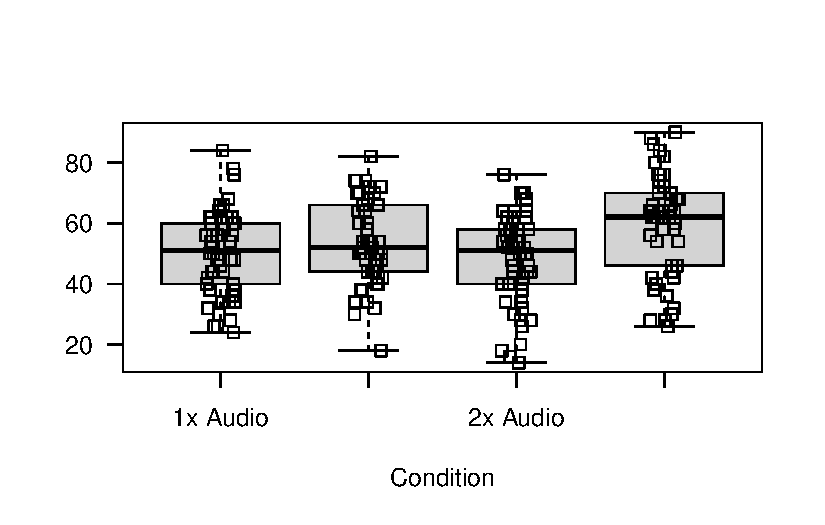
\includegraphics[keepaspectratio]{14_FE_Model_files/figure-pdf/unnamed-chunk-5-1.pdf}}

There are no clear signs of deviation from normality, the box-plots look
relatively symmetric. We could plot Q-Q plots for each treatment as
well. Let's do that for two of the treatments.

\begin{Shaded}
\begin{Highlighting}[]
\FunctionTok{par}\NormalTok{(}\AttributeTok{mfrow=}\FunctionTok{c}\NormalTok{(}\DecValTok{1}\NormalTok{,}\DecValTok{2}\NormalTok{)) }\CommentTok{\# splitting the plotting window into 1 row with 2 columns}

\FunctionTok{qqnorm}\NormalTok{(data}\SpecialCharTok{$}\NormalTok{Accuracy[data}\SpecialCharTok{$}\NormalTok{Condition }\SpecialCharTok{==} \StringTok{"1x Audio"}\NormalTok{], }\AttributeTok{pty =} \DecValTok{4}\NormalTok{, }\AttributeTok{col =}\StringTok{"blue"}\NormalTok{, }\AttributeTok{main =} \StringTok{"1x Audio"}\NormalTok{)}
\FunctionTok{qqline}\NormalTok{(data}\SpecialCharTok{$}\NormalTok{Accuracy[data}\SpecialCharTok{$}\NormalTok{Condition }\SpecialCharTok{==} \StringTok{"1x Audio"}\NormalTok{], }\AttributeTok{col =} \StringTok{"red"}\NormalTok{)}

\FunctionTok{qqnorm}\NormalTok{(data}\SpecialCharTok{$}\NormalTok{Accuracy[data}\SpecialCharTok{$}\NormalTok{Condition }\SpecialCharTok{==} \StringTok{"1x Audio{-}Visual"}\NormalTok{], }\AttributeTok{pty =} \DecValTok{4}\NormalTok{, }\AttributeTok{col =}\StringTok{"blue"}\NormalTok{, }\AttributeTok{main =} \StringTok{"1x Audio{-}Visual"}\NormalTok{)}
\FunctionTok{qqline}\NormalTok{(data}\SpecialCharTok{$}\NormalTok{Accuracy[data}\SpecialCharTok{$}\NormalTok{Condition }\SpecialCharTok{==} \StringTok{"1x Audio{-}Visual"}\NormalTok{], }\AttributeTok{col =} \StringTok{"red"}\NormalTok{)}
\end{Highlighting}
\end{Shaded}

\pandocbounded{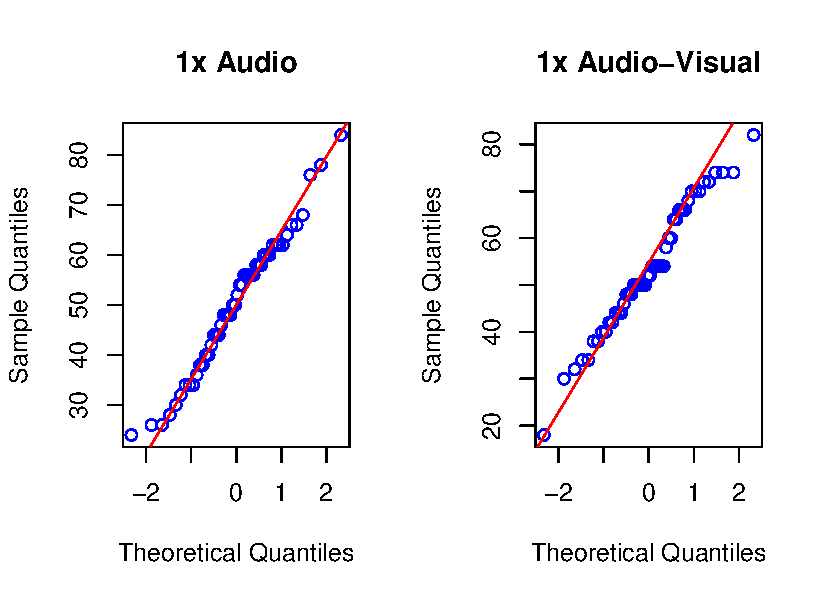
\includegraphics[keepaspectratio]{14_FE_Model_files/figure-pdf/unnamed-chunk-6-1.pdf}}

No worrisome patterns! Next, the box-plots also suggest that there are
no outliers and there are no clear indications that the assumption of
equal population variance is not reasonable. Let's have a look a the
standard deviations.

\begin{Shaded}
\begin{Highlighting}[]
\FunctionTok{sort}\NormalTok{(}\FunctionTok{tapply}\NormalTok{(data}\SpecialCharTok{$}\NormalTok{Accuracy, data}\SpecialCharTok{$}\NormalTok{Condition, sd))}
\end{Highlighting}
\end{Shaded}

\begin{verbatim}
1x Audio-Visual        1x Audio        2x Audio 2x Audio-Visual 
       13.71690        14.01084        14.93064        16.76386 
\end{verbatim}

The ratio of the smallest to largest is roughly 1.22 which is much
smaller than five. Lastly, we need to check the assumption of
independence. We start by assuming that the order in which the data are
in the data set is the order in which the measurements were taken and we
construct a Cleveland dot chart.

\begin{Shaded}
\begin{Highlighting}[]
\FunctionTok{dotchart}\NormalTok{(data}\SpecialCharTok{$}\NormalTok{Accuracy, }\AttributeTok{ylab =} \StringTok{"Order of observation"}\NormalTok{, }\AttributeTok{xlab =}\StringTok{"Post treatment test score"}\NormalTok{)}
\end{Highlighting}
\end{Shaded}

\pandocbounded{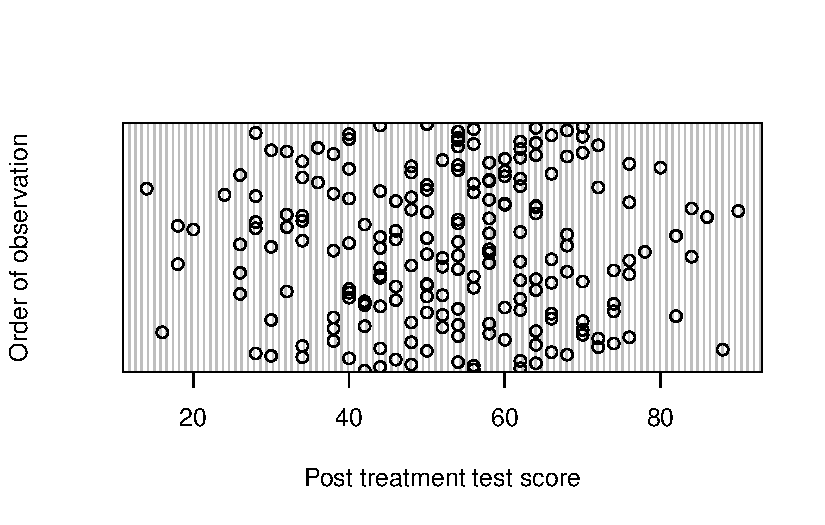
\includegraphics[keepaspectratio]{14_FE_Model_files/figure-pdf/unnamed-chunk-8-1.pdf}}

No clear patterns in the measurements, so no reason to suspect any
dependence between successive measurements. The students were randomly
assigned to each group and there are no other reasons to believe that
independence was violated based on the description of the experiment.

With all the assumptions checked, we can move onto fitting the linear
model to our data and inspecting the model estimates. Here is the model
equation:

\[ \text{Accuracy}_{ijk} = \mu + \text{Speed}_i + \text{Content.Type}_j + \text{(Speed:Content.Type)}_{ij} + e_{ijk} \]

where,

\[
\begin{aligned}
    i &= 1,2\text{ and }j = 1,2\\
    e_{ijk} &= \text{random error with } e_{ijk} \sim N(0, \sigma^2) \\
\end{aligned}
\]

In R, we fit the model like this:

\begin{Shaded}
\begin{Highlighting}[]
\NormalTok{model }\OtherTok{\textless{}{-}} \FunctionTok{aov}\NormalTok{(Accuracy }\SpecialCharTok{\textasciitilde{}}\NormalTok{ Speed }\SpecialCharTok{+}\NormalTok{ Content.Type }\SpecialCharTok{+}\NormalTok{ Speed}\SpecialCharTok{:}\NormalTok{Content.Type, }\AttributeTok{data =}\NormalTok{ data)}
\FunctionTok{model.tables}\NormalTok{(model, }\AttributeTok{type =} \StringTok{"means"}\NormalTok{, }\AttributeTok{se =} \ConstantTok{TRUE}\NormalTok{)}
\end{Highlighting}
\end{Shaded}

\begin{verbatim}
Tables of means
Grand mean
      
52.78 

 Speed 
Speed
    1     2 
54.94 50.62 

 Content.Type 
Content.Type
  Audio-Only Audio-Visual 
       49.10        56.46 

 Speed:Content.Type 
     Content.Type
Speed Audio-Only Audio-Visual
    1 50.32      59.56       
    2 47.88      53.36       

Standard errors for differences of means
        Speed Content.Type Speed:Content.Type
        2.108        2.108              2.981
replic.   100          100                 50
\end{verbatim}

R allows a convenient shorthand for this type of model. Instead of
typing out all three terms, you can shorten the right hand side of the
formula to \texttt{Speed*Content.Type}. The \texttt{*} operator
indicates to R that we want main effects and interaction effects. Try it
yourself to see that you get the same result.

We extract the treatment means as before. The grand mean is shown first.
Now with a factorial treatment structure, we get the mean values for
each level of the treatment factors included and the treatment means. In
the output below, we see the means of the 1x and 2x speed followed by
the means for the levels of content type. Lastly, the treatment means
are presented in a 2 by 2 matrix format. The treatment ``1x Audio Only''
had a mean accuracy of 50.32, ``2x Audio-Only'' mean response is 47.8,
and so on. And then lastly, the standard errors for differences between
means.

We can also extract the estimated effects as before.

\begin{Shaded}
\begin{Highlighting}[]
\FunctionTok{model.tables}\NormalTok{(model, }\AttributeTok{type =} \StringTok{"effects"}\NormalTok{, }\AttributeTok{se =} \ConstantTok{TRUE}\NormalTok{)}
\end{Highlighting}
\end{Shaded}

\begin{verbatim}
Tables of effects

 Speed 
Speed
    1     2 
 2.16 -2.16 

 Content.Type 
Content.Type
  Audio-Only Audio-Visual 
       -3.68         3.68 

 Speed:Content.Type 
     Content.Type
Speed Audio-Only Audio-Visual
    1 -0.94       0.94       
    2  0.94      -0.94       

Standard errors of effects
        Speed Content.Type Speed:Content.Type
        1.490        1.490              2.108
replic.   100          100                 50
\end{verbatim}

First we get the main effects for \texttt{Speed} and
\texttt{Content.Type}. Then we get the interaction effects and standard
errors. Let's check that we understand how these interaction effects are
calculated. Remember:

\[(AB)_{ij} = \bar{Y}_{ij} - (\mu + A_i + B_j) \]

So for treatment \(i = 1\) and \(j=1\), the equation becomes:

\[\hat{(AB)}_{11} = \bar{Y}_{11} - (\hat{\mu} + \hat{A}_1 + \hat{B}_1) \]

We go by the dimensions of the matrix returned by R, so then treatment
\(i = 1\) and \(j=1\) is ``1x Audio-Only''. Substituting the estimated
values:

\[
\begin{aligned}
(AB)_{11} &= 50.32 - (52.78 + 2.16 -3.68) \\
&= -0.94
\end{aligned}
\]

Which is what R outputs as well. Now, we want to ask is there evidence
for an interaction effect? To do this we need to construct the ANOVA
table.

\chapter{ANOVA}\label{anova}

The model for a factorial experiment with two treatment factors was:

\[
Y_{ijk} = \mu + A_i + C_j + (AC)_{ij} + e_{ijk}
\]

If we move \(\mu\) to the left-hand side of the equation, we get:

\[
Y_{ijk} - \mu = A_i + C_j + (AC)_{ij} + e_{ijk}
\]

Now, each of the terms on the RHS is a deviation from a mean.

\begin{itemize}
\tightlist
\item
  The main effects come from the overall mean \(\mu\),\\
\item
  The interaction effects from \(\mu + A_i + C_j\),\\
\item
  The error terms from the treatment means.
\end{itemize}

We can square and sum the corresponding observed deviations and obtain
sums of squares. For a \textbf{balanced} factorial experiment, the total
sum of squares on the LHS can be split into four parts, corresponding
to:

\begin{enumerate}
\def\labelenumi{\arabic{enumi}.}
\tightlist
\item
  Main effects of factor \textbf{A},
\item
  Main effects of factor \textbf{C},
\item
  Interaction between \textbf{A} and \textbf{C} effects,
\item
  Error.
\end{enumerate}

\[
SS_{total} = SS_A + SS_C + SS_{AC} + SS_E
\]

The degrees of freedom for these sums of squares are:

\[
abn - 1 = (a - 1) + (b - 1) + (a - 1)(b - 1) + ab(n - 1)
\]

where \(n\) is the number of replicates per treatment. The degrees of
freedom on the right-hand side add up to the total degrees of freedom.
Once again, we summarise all this in a table.

\subsection*{ANOVA Table}\label{anova-table-1}
\addcontentsline{toc}{subsection}{ANOVA Table}

The following table summarizes the partitioning of variation:

\begin{longtable}[]{@{}
  >{\raggedright\arraybackslash}p{(\linewidth - 8\tabcolsep) * \real{0.2000}}
  >{\raggedright\arraybackslash}p{(\linewidth - 8\tabcolsep) * \real{0.2000}}
  >{\raggedright\arraybackslash}p{(\linewidth - 8\tabcolsep) * \real{0.2000}}
  >{\raggedright\arraybackslash}p{(\linewidth - 8\tabcolsep) * \real{0.2000}}
  >{\raggedright\arraybackslash}p{(\linewidth - 8\tabcolsep) * \real{0.2000}}@{}}
\toprule\noalign{}
\begin{minipage}[b]{\linewidth}\raggedright
Source
\end{minipage} & \begin{minipage}[b]{\linewidth}\raggedright
SS
\end{minipage} & \begin{minipage}[b]{\linewidth}\raggedright
df
\end{minipage} & \begin{minipage}[b]{\linewidth}\raggedright
MS
\end{minipage} & \begin{minipage}[b]{\linewidth}\raggedright
F
\end{minipage} \\
\midrule\noalign{}
\endhead
\bottomrule\noalign{}
\endlastfoot
A Main Effects & \(SS_A = nb \sum_i (\bar{Y}_{i..} - \bar{Y}_{...})^2\)
& \((a - 1)\) & \(MS_A\) & \(\frac{MS_A}{MS_E}\) \\
C Main Effects & \(SS_C = na \sum_j (\bar{Y}_{.j.} - \bar{Y}_{...})^2\)
& \((b - 1)\) & \(MS_C\) & \(\frac{MS_C}{MS_E}\) \\
AC Interactions &
\(SS_{AC} = n \sum_{ij} (\bar{Y}_{ij.} - \bar{Y}_{i..} - \bar{Y}_{.j.} + \bar{Y}_{...})^2\)
& \((a - 1)(b - 1)\) & \(MS_{AC}\) & \(\frac{MS_{AC}}{MS_E}\) \\
Error & \(SS_E = \sum_{ijk} (Y_{ijk} - \bar{Y}_{ij.})^2\) &
\(ab(n - 1)\) & \(MSE\) & - \\
Total & \(SS_{total} = \sum_{ijk} (Y_{ijk} - \bar{Y}_{...})^2\) &
\(abn - 1\) & - & - \\
\end{longtable}

There are three F-tests in this ANOVA table.

\begin{enumerate}
\def\labelenumi{\arabic{enumi}.}
\tightlist
\item
  \(H_{AB} : (\alpha\beta)_{ij} = 0\) for all \(i\) and \(j\) (Factors A
  and B do not interact)
\item
  \(H_A : \alpha_i = 0 \quad i = 1, \dots, a\) (Factor A has no main
  effects)
\item
  \(H_B : \beta_j = 0 \quad j = 1, \dots, b\) (Factor B has no main
  effects)
\end{enumerate}

The alternative hypothesis is, in each case, that at least one of the
parameters considered is non-zero.

While discussing interactions, we saw that sometimes, with strong
interaction effects, the main effects of a factor may disappear (be
close to zero). But this does not mean that the factor has no effect. On
the contrary, it has an effect on the response; the effects just differ
over the levels of the other factor and may average out.

Therefore, we usually start by testing the interaction effects. If there
is evidence for the presence of interactions, we have to examine the
main effects with this in mind, i.e., be careful with the interpretation
of the main effects. Some people say that it becomes meaningless to test
for main effects if there is evidence of interactions. However, this
depends on what we want to know. The main effects still tell us whether
or not the average response changes with changing levels of the factor.

The \textbf{F-ratio} always has the mean square for error in the
denominator. As before, it is a ratio of two variance estimates, and in
each case, it can be seen as a \textbf{signal-to-noise ratio}: how large
are the effects relative to the experimental error variance?

\section{Back to the example}\label{back-to-the-example-1}

Before we inspect the ANOVA table for the working example, we need to
check the assumptions about the errors after model fitting. We do this
by inspecting the residuals.

\begin{Shaded}
\begin{Highlighting}[]
\FunctionTok{par}\NormalTok{(}\AttributeTok{mfrow =} \FunctionTok{c}\NormalTok{(}\DecValTok{1}\NormalTok{,}\DecValTok{2}\NormalTok{))}
\FunctionTok{plot}\NormalTok{(model, }\AttributeTok{which =} \DecValTok{1}\NormalTok{)}
\FunctionTok{plot}\NormalTok{(model, }\AttributeTok{which =} \DecValTok{2}\NormalTok{)}
\end{Highlighting}
\end{Shaded}

\pandocbounded{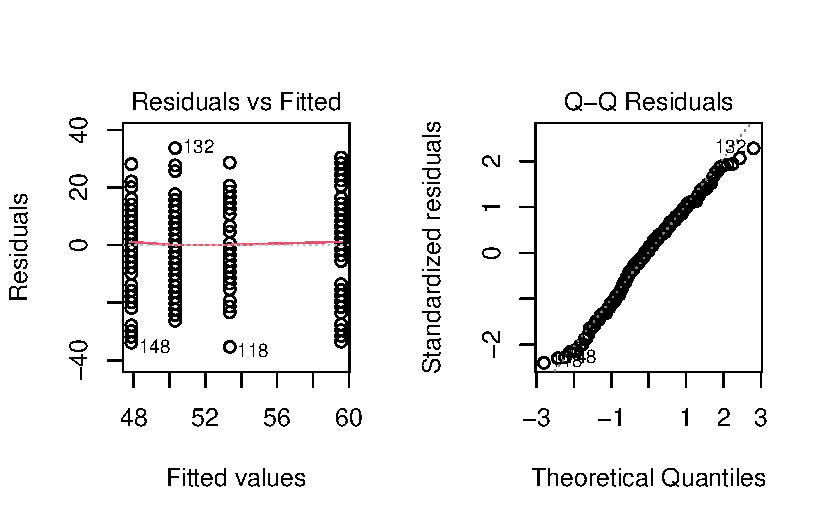
\includegraphics[keepaspectratio]{16_FE_ANOVA_files/figure-pdf/unnamed-chunk-1-1.pdf}}

There are no clear violations, in the first plot, the residuals appear
to be centered around zero and the spread is reasonably equal across
groups. The second plot is a Q-Q plot of the residuals which shows
nothing worrisome. Remember we can also plot a histogram of the
residuals to check normality.

For the independence assumption, we construct the dot chart once again
but with the residuals.

\begin{Shaded}
\begin{Highlighting}[]
\FunctionTok{dotchart}\NormalTok{(model}\SpecialCharTok{$}\NormalTok{residuals) }\CommentTok{\# note the different way of extracting residuals!}
\end{Highlighting}
\end{Shaded}

\pandocbounded{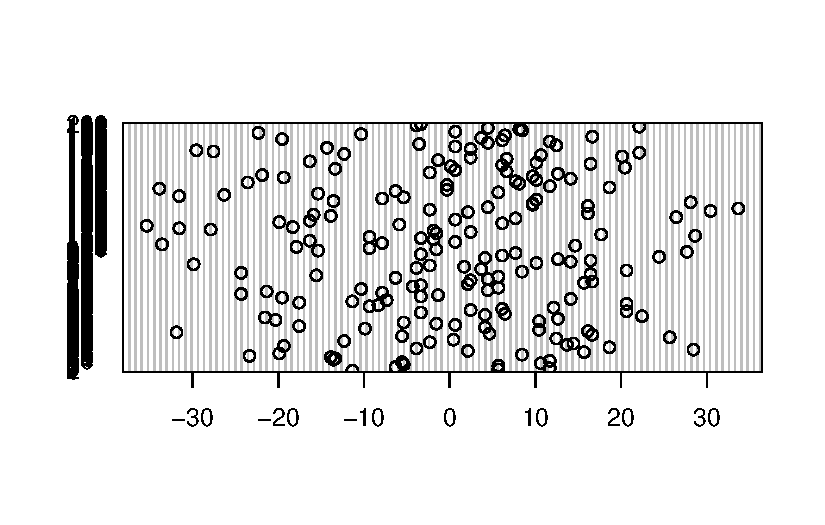
\includegraphics[keepaspectratio]{16_FE_ANOVA_files/figure-pdf/unnamed-chunk-2-1.pdf}}

The y-axis is messy but we can ignore that, it shows the index of each
observation and there are 200 hence why it overlaps so much. The
residuals look uniform, there are no systematic patterns or trends in
the plot.

Let's see what the ANOVA table looks like for our working example.

\begin{Shaded}
\begin{Highlighting}[]
\FunctionTok{summary}\NormalTok{(model)}
\end{Highlighting}
\end{Shaded}

\begin{verbatim}
                    Df Sum Sq Mean Sq F value   Pr(>F)    
Speed                1    933   933.1   4.201 0.041724 *  
Content.Type         1   2708  2708.5  12.195 0.000592 ***
Speed:Content.Type   1    177   176.7   0.796 0.373485    
Residuals          196  43532   222.1                     
---
Signif. codes:  0 '***' 0.001 '**' 0.01 '*' 0.05 '.' 0.1 ' ' 1
\end{verbatim}

Verify that the degrees of freedom are what you expected! First, we look
at the interaction. The F-value is quite small which leads to a large
p-value of 0.37. This means that we really have no evidence against the
null hypothesis that the factors interact. There is some evidence for a
main effect of Speed but there is much stronger evidence as indicated by
the small p-value for a main effect of lecture modality.

\chapter{Contrasts}\label{contrasts-2}

There are two approaches to analysing data from experiments. The first
is to construct a set of a-priori contrasts, test these, and perhaps
afterwards use unplanned comparisons to see if there are any other
interesting treatment effects or differences that we might want to
follow up with in a future experiment.

The second approach is an analysis of variance (ANOVA). This usually
tests much more general hypotheses about the presence of main and
interaction effects. The two approaches are not mutually exclusive, but
if the questions we are interested in are not answered by an analysis of
variance, we should concentrate on the contrasts. The two approaches may
also give what seem to be different answers.

For example, from the ANOVA F-test, we may see no evidence for
interactions, but if we look at specific contrasts for interactions,
there is evidence. This can happen; it is not a mistake in the methods,
it is just a difference in the hypotheses that are being tested.

Often, an ANOVA is expected in journal publications and research
reports, even if it does not answer the specific research questions. The
more specific questions are answered by constructing confidence
intervals or tests for contrasts.

Let's revisit the specific research questions for the working example:

\begin{enumerate}
\def\labelenumi{\arabic{enumi}.}
\tightlist
\item
  Does lecture modality have an effect on comprehension?
\item
  Does playback speed have an effect on comprehension?
\item
  Is there an interaction effect of modality and playback speed on
  comprehension?
\end{enumerate}

With these question, conducting an ANOVA is enough. We simply want to
know if there are any main effects or interaction effects. We have
answered that with the ANOVA above. But what if the questions were a bit
more specific:

\begin{enumerate}
\def\labelenumi{\arabic{enumi}.}
\tightlist
\item
  Does audio-visual content increase comprehension?
\item
  Does increased playback speed decrease comprehension?
\item
  Is the effect of playback speed improved by audio-visual content?
\end{enumerate}

So far we have only contrasted two treatments. Sometimes we want to
compare groups of treatments to one another. More generally, a contrast
is defined as a linear combination of the parameters where the
coefficients add up to zero:

\[L = \sum_1^a h_iA_i\]

such that \(\sum_1^a h_i = 0\). This ensures a fair comparison. For
example, in a comparison of two group means we have:

\[ L = \mu_1 - \mu_2 = 1\times \mu + (-1) \times \mu_2\] Here, the
coefficients are \(h_1 = +1\) and \(h_2 = -1\) which sum to zero. This
simple difference is the simplest form of a contrast. Effectively,
\(\sum_1^a h_i = 0\) represents the null hypothesis, that the difference
equals 0.

Let's start with the first question. Remember the treatments were:

\begin{enumerate}
\def\labelenumi{\arabic{enumi}.}
\tightlist
\item
  1x Audio-Only (1AO)
\item
  2x Audio-Only (2AO)
\item
  1x Audio-Visual (1AV)
\item
  2x Audio-Visual (2AV)
\end{enumerate}

To answer the first question, our contrast should compare Audio-Visual
vs.~Audio-Only and we do this by averaging over the levels of playback
speed.

First we compute the average response for the two levels of content
type, AV and AO.

\[\frac{(\mu_{1AV} + \mu_{2AV})}{2}\]

\[\frac{(\mu_{1AO} + \mu_{2AO})}{2}\]

Now we are comparing groups of means. The first group contains the means
for all treatments that included Audio-Visual level and the second
contains the Audio-Only level. We are asking whether the AV level
increased comprehension. So we are testing:

\marginnote{\begin{footnotesize}

We could specify the difference either way, that is AO - AV. Then we
would be doing a one-sided lower tailed test.

\end{footnotesize}}

\[H_0: \frac{(\mu_{1AV} + \mu_{2AV})}{2} = \frac{(\mu_{1AO} + \mu_{2AO})}{2}\]

\[
H_1: \frac{(\mu_{1AV} + \mu_{2AV})}{2} > \frac{(\mu_{1AO} + \mu_{2AO})}{2} <=> \frac{(\mu_{1AV} + \mu_{2AV})}{2} - \frac{(\mu_{1AO} + \mu_{2AO})}{2} > 0
\]

The coefficients of the contrast sum to zero:

\[
\begin{aligned}
&\frac{(\mu_{AV1} + \mu_{AV2}) - (\mu_{AO1} + \mu_{AO2})}{2} \\
&\frac{(1) \mu_{AV1} + (1) \mu_{AV2} + (-1) \mu_{AO1} + (-1) \mu_{AO2}}{2} \\ 
& (0.5) \mu_{AV1} + (0.5) \mu_{AV2} + (-0.5) \mu_{AO1} + (-0.5) \mu_{AO2} \\
&0.5+.0.5-0.5-0.5 = 0
\end{aligned}
\] This is a linear combination of the model parameters. What does the
contrast and coefficients look like for the second question? To test
whether playback speed decreases comprehension, we need to compare
treatments at 1x speed vs.~2x speed:

\[\frac{(\mu_{1AV} + \mu_{1AO})}{2} - \frac{(\mu_{2AO} + \mu_{2AV})}{2}\]
The coefficients sum to zero as before. This might be confusing but we
are simply grouping treatments together and comparing them. To compute
these contrasts in R, we first fit the model using lm() and extract the
treatment means using \texttt{emmeans} from the \texttt{emmeans}
package.

\begin{Shaded}
\begin{Highlighting}[]
\NormalTok{model\_reg }\OtherTok{\textless{}{-}} \FunctionTok{lm}\NormalTok{(Accuracy }\SpecialCharTok{\textasciitilde{}}\NormalTok{ Content.Type }\SpecialCharTok{*}\NormalTok{ Speed, }\AttributeTok{data =}\NormalTok{ data)}

\NormalTok{means }\OtherTok{\textless{}{-}} \FunctionTok{emmeans}\NormalTok{(model\_reg, }\SpecialCharTok{\textasciitilde{}}\NormalTok{Content.Type }\SpecialCharTok{*}\NormalTok{ Speed)}

\NormalTok{means}
\end{Highlighting}
\end{Shaded}

\begin{verbatim}
 Content.Type Speed emmean   SE  df lower.CL upper.CL
 Audio-Only       1   50.3 2.11 196     46.2     54.5
 Audio-Visual     1   59.6 2.11 196     55.4     63.7
 Audio-Only       2   47.9 2.11 196     43.7     52.0
 Audio-Visual     2   53.4 2.11 196     49.2     57.5

Confidence level used: 0.95 
\end{verbatim}

The \texttt{emmeans} function returns the treatment means, the standard
error, degrees of freedom and the bounds of 95\% confidence interval.
Now we want to perform the two contrasts using the means saved in the
object we created, \texttt{means}. First, note the order in which
\texttt{emmeans} outputs the treatments:

AO1, AV1, A02, AV2.

We are going to use this order and the coefficients were determined
earlier to perform the ocntrasts with the function \texttt{contrast()}
also from the package \texttt{emmeans}:

\begin{Shaded}
\begin{Highlighting}[]
\FunctionTok{contrast}\NormalTok{(means,}
         \FunctionTok{list}\NormalTok{(}
           \AttributeTok{c1 =} \FunctionTok{c}\NormalTok{(}\SpecialCharTok{{-}}\DecValTok{1}\NormalTok{,}\DecValTok{1}\NormalTok{,}\SpecialCharTok{{-}}\DecValTok{1}\NormalTok{,}\DecValTok{1}\NormalTok{)}\SpecialCharTok{/}\DecValTok{2}\NormalTok{, }\CommentTok{\# AV {-} AO}
           \AttributeTok{c2 =} \FunctionTok{c}\NormalTok{(}\DecValTok{1}\NormalTok{,}\DecValTok{1}\NormalTok{,}\SpecialCharTok{{-}}\DecValTok{1}\NormalTok{,}\SpecialCharTok{{-}}\DecValTok{1}\NormalTok{)}\SpecialCharTok{/}\DecValTok{2} \CommentTok{\# 2x {-} 1x}
\NormalTok{         ),}
         \AttributeTok{by =} \ConstantTok{NULL}\NormalTok{, }\AttributeTok{side =} \StringTok{"\textgreater{}"}\NormalTok{)}
\end{Highlighting}
\end{Shaded}

\begin{verbatim}
 contrast estimate   SE  df t.ratio p.value
 c1           7.36 2.11 196   3.492  0.0003
 c2           4.32 2.11 196   2.050  0.0209

P values are right-tailed 
\end{verbatim}

We supply the emmeans object \texttt{means} and then a list of contrasts
we call \texttt{c1} and \texttt{c2} corresponding to the first and
second question. Each contrast consists of the coefficients in the order
in which the means appear in the \texttt{means} object and the scaling
by 2. Then we need to specify \texttt{by\ =\ NULL} because we have
manually coded the contrasts and don't need to specify by which factor
the contrasts should made. Lastly, we specify the type of test we want,
that is, is it one sided or two sided. If it is one-sided, in which
direction? We have specifically constructed the contrasts so that both
are ``one-sided greater than''.

The output shows the estimate of each contrast, the standard error of
the difference in means, t-value and associated p-value. For the first
contrast we see the difference in comprehension scores between the
Audio-Visual and Audio-Only groups was 7.36, this means that the average
response in the Audio-Visual group was higher than the average response
in the Audio-Only group. We see that the p-value to test this contrast
is 0.0003 which is extremely small, so it is unlikely that the
difference in mean response is due to chance. There is strong evidence
to indicate that the audio-visual type increased the mean response, the
estimate of this the difference between groups is 7.36\% (\(t=3.492\),
\(df = 196\), \(p = 0.0003\)).

For the second contrast, the p-value still provides sufficient evidence
against the null hypothesis that the difference is zero but it is not as
strong as for the first contrast. However, we are still satisfied with
the evidence against \(H_0\). The 2x speed decreased the average
accuracy (averaged over the levels of content type) by 4.32\%
(\(t=-2.050\), \(df = 196\), \(p = 0.021\)).

When we have factors with two levels (as we do here) and we conduct two
sided contrasts, then the contrast is equivalent to testing for the
presence of main effects which what the ANOVA table does! Remember we
said that the ANOVA is an extension of the t-test and with two levels.
Let's go through this step-by-step:

\begin{itemize}
\tightlist
\item
  We conducted one-sided tests.
\item
  If we conducted two-sided tests, the results would be the same as in
  ANOVA table.
\item
  This is because when we have two levels per treatment factor, the
  contrasts are equivalent to testing whether there are main effects of
  Speed and Content.Type.
\end{itemize}

Since we conducted one-sided tests, the p-value is has been split
between the tails. To get to the value of the p-value for a two-sided
tests, we multiply the one-sided p-value by 2.

\begin{Shaded}
\begin{Highlighting}[]
\CommentTok{\# For AV {-} AO = 0}

\FloatTok{0.0003}\SpecialCharTok{*}\DecValTok{2}
\end{Highlighting}
\end{Shaded}

\begin{verbatim}
[1] 6e-04
\end{verbatim}

\begin{Shaded}
\begin{Highlighting}[]
\CommentTok{\# For 1 {-} 2 = 0}

\FloatTok{0.0209} \SpecialCharTok{*} \DecValTok{2}
\end{Highlighting}
\end{Shaded}

\begin{verbatim}
[1] 0.0418
\end{verbatim}

Check that these are the same as in the ANOVA table. The test statistics
are also related in this case, \(t^2 = F\).

Let's answer the third question. Since we have two levels per factor,
this question is asking about the interaction. The contrast for the
interaction should compare the \emph{difference between audio-visual and
audio-only in the two levels of playback speed}:

At 1x playback speed, the effect of content type is given by:

\[
(\mu_{AV1} - \mu_{AO1})
\]

At 2x playback speed, the effect of content type is given by:

\[
(\mu_{AV2} - \mu_{AO2})
\]

Now to examine whether the effect of content type is consistent across
playback speeds, we compute:

\[
\begin{aligned}
&(\mu_{AV1} - \mu_{AO1}) - (\mu_{AV2} - \mu_{AO2})\\
& = \mu_{AV1} - \mu_{AO1} - \mu_{AV2} + \mu_{AO2}
\end{aligned}
\]

This contrast assesses whether the difference between Audio-Visual and
Audio-Only is the same at 1x and 2x speeds.

\marginnote{\begin{footnotesize}

We are not dividing by two because we are not averaging across
conditions, we are computing the difference of two differences.

\end{footnotesize}}

\begin{Shaded}
\begin{Highlighting}[]
\FunctionTok{contrast}\NormalTok{(means,}
         \FunctionTok{list}\NormalTok{(}
           \AttributeTok{c3 =} \FunctionTok{c}\NormalTok{(}\SpecialCharTok{{-}}\DecValTok{1}\NormalTok{, }\DecValTok{1}\NormalTok{, }\DecValTok{1}\NormalTok{,}\SpecialCharTok{{-}}\DecValTok{1}\NormalTok{) }\CommentTok{\# interaction}
\NormalTok{         ),}
         \AttributeTok{by =} \ConstantTok{NULL}\NormalTok{)}
\end{Highlighting}
\end{Shaded}

\begin{verbatim}
 contrast estimate   SE  df t.ratio p.value
 c3           3.76 4.22 196   0.892  0.3735
\end{verbatim}

We get the same p-value as in the ANOVA table which indicates a lack of
evidence against the null hypothesis, there is no evidence to suggest
that the two factors interact (\(t=0.892\), \(df = 196\),
\(p = 0.374\)).

In practice, we would test the interaction first and then interpret the
main effects if there is evidence to support their presence. Here we
have done it this way around purely for educational purposes.

We can also visualise the interaction (especially useful for
understanding the interaction if there is evidence for one!). There is a
built-in function in R that can do this for us, but it will be useful to
construct the plot from scratch to ensure you understand what it
visualises.

Have a look at the data set again.

\begin{Shaded}
\begin{Highlighting}[]
\FunctionTok{head}\NormalTok{(data)}
\end{Highlighting}
\end{Shaded}

\begin{verbatim}
  Participant.ID       Condition Speed Content.Type Accuracy
1     945445adf5 1x Audio-Visual     2 Audio-Visual       42
2     23afb88ef3        1x Audio     1   Audio-Only       56
3     1bc24e0480        1x Audio     1   Audio-Only       62
4     4fbdbd41a5        1x Audio     1   Audio-Only       44
5     442adf227a        1x Audio     1   Audio-Only       56
6     3ca9d09e2e 1x Audio-Visual     2 Audio-Visual       48
\end{verbatim}

We want to visualise the response per treatment for each combination of
Speed and Content.Type (which is already combined in the column
Condition). We did this with the \texttt{emmeans} function and stored
the treatment means in the object \texttt{means}! To use it to visualise
the treatment means we need to convert to a data frame, currently it is
something called a ``emmGrid''

\begin{Shaded}
\begin{Highlighting}[]
\NormalTok{means }
\end{Highlighting}
\end{Shaded}

\begin{verbatim}
 Content.Type Speed emmean   SE  df lower.CL upper.CL
 Audio-Only       1   50.3 2.11 196     46.2     54.5
 Audio-Visual     1   59.6 2.11 196     55.4     63.7
 Audio-Only       2   47.9 2.11 196     43.7     52.0
 Audio-Visual     2   53.4 2.11 196     49.2     57.5

Confidence level used: 0.95 
\end{verbatim}

\begin{Shaded}
\begin{Highlighting}[]
\FunctionTok{class}\NormalTok{(means)}
\end{Highlighting}
\end{Shaded}

\begin{verbatim}
[1] "emmGrid"
attr(,"package")
[1] "emmeans"
\end{verbatim}

It is easy to convert the object to a data frame:

\begin{Shaded}
\begin{Highlighting}[]
\NormalTok{means\_data }\OtherTok{\textless{}{-}} \FunctionTok{data.frame}\NormalTok{(means)}
\end{Highlighting}
\end{Shaded}

We need to decide which factor will be on the x-axis, let's do Speed.
Below, I use a new package called \texttt{ggplot2} to visualise the
data. It creates nicer looking plots and is more intuitive in my
opinion. If you want to see how to use base R to plot this, see the code
at the end of this section.

\begin{Shaded}
\begin{Highlighting}[]
\CommentTok{\# install.packages("ggplot2")}
\FunctionTok{library}\NormalTok{(ggplot2)}

\CommentTok{\# Create the ggplot with interaction lines}
\FunctionTok{ggplot}\NormalTok{(means\_data, }\FunctionTok{aes}\NormalTok{(}\AttributeTok{x =} \FunctionTok{factor}\NormalTok{(Speed), }\AttributeTok{y =}\NormalTok{ emmean, }\AttributeTok{colour =}\NormalTok{ Content.Type, }\AttributeTok{group =}\NormalTok{ Content.Type)) }\SpecialCharTok{+}
  \FunctionTok{geom\_point}\NormalTok{(}\AttributeTok{size =} \DecValTok{3}\NormalTok{) }\SpecialCharTok{+}     \CommentTok{\# Add points for each Content Type}
  \FunctionTok{geom\_line}\NormalTok{(}\AttributeTok{linewidth =} \DecValTok{1}\NormalTok{) }\SpecialCharTok{+}      \CommentTok{\# Connect points with lines}
  \FunctionTok{labs}\NormalTok{(}\AttributeTok{title =} \StringTok{"Interaction Plot: Speed vs Content Type"}\NormalTok{,}
       \AttributeTok{x =} \StringTok{"Speed"}\NormalTok{,}
       \AttributeTok{y =} \StringTok{"Mean Response"}\NormalTok{) }\SpecialCharTok{+}
  \FunctionTok{scale\_y\_continuous}\NormalTok{(}\AttributeTok{limits =}\FunctionTok{c}\NormalTok{(}\DecValTok{35}\NormalTok{,}\DecValTok{65}\NormalTok{)) }\SpecialCharTok{+} \CommentTok{\# to visualse the magnitude a bit better}
  \FunctionTok{theme\_minimal}\NormalTok{()}
\end{Highlighting}
\end{Shaded}

\pandocbounded{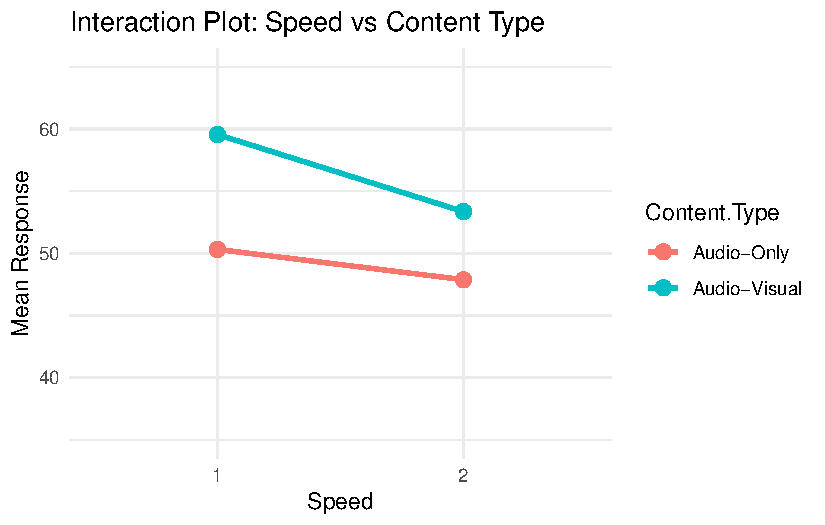
\includegraphics[keepaspectratio]{17_FE_Contrasts_files/figure-pdf/unnamed-chunk-8-1.pdf}}

The \texttt{aes()} function maps Speed to the x-axis, Mean Response to
the y-axis, and uses Content Type for color and grouping.
\texttt{geom\_point(size\ =\ 3)} adds individual data points, while
\texttt{geom\_line(size\ =\ 1)} connects them to show trends. The
\texttt{labs()} function provides axis labels and a title, and
\texttt{theme\_minimal()} specifies the theme for the plot.

\marginnote{\begin{footnotesize}

If you want to know more about how to visualise data with
\texttt{ggplot2} have a look at this
\href{https://ggplot2.tidyverse.org/}{link}. There are plenty of
resources mentioned.

\end{footnotesize}}

It is evident that increasing Speed has a negative effect on the
response, and switching from Audio-Visual to Audio-Only content reduces
the mean response. When moving from 1x to 2x Speed in the Audio-Visual
condition, the response decreases. A similar decline is observed for the
Audio-Only condition. Although the decrease appears slightly larger for
Audio-Visual than for Audio-Only, the difference is not substantial
enough to conclude a significant interaction effect between Speed and
Content Type as evidenced by the ANOVA and contrasts we did before.

\section{Conclusion}\label{conclusion}

\begin{Shaded}
\begin{Highlighting}[]
\CommentTok{\# Set up an empty plot}
\FunctionTok{plot}\NormalTok{(means\_data}\SpecialCharTok{$}\NormalTok{Speed[means\_data}\SpecialCharTok{$}\NormalTok{Content.Type }\SpecialCharTok{==} \StringTok{"Audio{-}Visual"}\NormalTok{], }
\NormalTok{     means\_data}\SpecialCharTok{$}\NormalTok{emmean[means\_data}\SpecialCharTok{$}\NormalTok{Content.Type }\SpecialCharTok{==} \StringTok{"Audio{-}Visual"}\NormalTok{], }
     \AttributeTok{type =} \StringTok{"o"}\NormalTok{, }
     \AttributeTok{col =} \StringTok{"\#F79256"}\NormalTok{, }
     \AttributeTok{pch =} \DecValTok{16}\NormalTok{, }
     \AttributeTok{ylim =} \FunctionTok{range}\NormalTok{(means\_data}\SpecialCharTok{$}\NormalTok{emmean), }
     \AttributeTok{xlab =} \StringTok{"Speed"}\NormalTok{, }
     \AttributeTok{ylab =} \StringTok{"Mean Response"}\NormalTok{, }
     \AttributeTok{main =} \StringTok{"Interaction Plot: Speed vs Content Type"}\NormalTok{,}
     \AttributeTok{xaxt =} \StringTok{"n"}\NormalTok{)}

\CommentTok{\# {-} plot(...) initializes the graph using Speed as the x{-}axis and Mean Response as the y{-}axis.}
\CommentTok{\# {-} The subset \textasciigrave{}means\_data$Speed[means\_data$ContentType == "Audio{-}Visual"]\textasciigrave{} extracts only Audio{-}Visual data to plot the first line.}
\CommentTok{\# {-} type = "o" specifies that both points and lines should be drawn.}
\CommentTok{\# {-} ylim = range(means\_data$emmean) ensures that the y{-}axis spans the full range of data.}
\CommentTok{\# {-} xaxt = "n" suppresses the default x{-}axis, allowing for manual customization in the next step.}
\CommentTok{\# }
\CommentTok{\# Since the x{-}axis represents discrete categories (Speed levels), we manually specify the tick labels with the function \textasciigrave{}axis\textasciigrave{} and then we overlay the means for the Audio{-}Only groups with \textasciigrave{}points\textasciigrave{}. Lastly, we add a legend. }

\CommentTok{\# Add x{-}axis labels manually}
\FunctionTok{axis}\NormalTok{(}\DecValTok{1}\NormalTok{, }\AttributeTok{at =} \FunctionTok{unique}\NormalTok{(}\FunctionTok{as.numeric}\NormalTok{(means\_data}\SpecialCharTok{$}\NormalTok{Speed)), }\AttributeTok{labels =} \FunctionTok{unique}\NormalTok{(means\_data}\SpecialCharTok{$}\NormalTok{Speed))}

\CommentTok{\# Add Audio{-}Only group}
\FunctionTok{points}\NormalTok{(means\_data}\SpecialCharTok{$}\NormalTok{Speed[means\_data}\SpecialCharTok{$}\NormalTok{Content.Type }\SpecialCharTok{==} \StringTok{"Audio{-}Only"}\NormalTok{], }
\NormalTok{       means\_data}\SpecialCharTok{$}\NormalTok{emmean[means\_data}\SpecialCharTok{$}\NormalTok{Content.Type }\SpecialCharTok{==} \StringTok{"Audio{-}Only"}\NormalTok{], }
       \AttributeTok{col =} \StringTok{"\#5BC0EB"}\NormalTok{, }
       \AttributeTok{pch =} \DecValTok{16}\NormalTok{, }
       \AttributeTok{type =} \StringTok{"o"}\NormalTok{)}

\CommentTok{\# Add legend}
\FunctionTok{legend}\NormalTok{(}\StringTok{"topright"}\NormalTok{, }\AttributeTok{legend =} \FunctionTok{c}\NormalTok{(}\StringTok{"Audio{-}Visual"}\NormalTok{, }\StringTok{"Audio{-}Only"}\NormalTok{), }\AttributeTok{col =} \FunctionTok{c}\NormalTok{(}\StringTok{"\#F79256"}\NormalTok{, }\StringTok{"\#5BC0EB"}\NormalTok{), }\AttributeTok{pch =} \DecValTok{16}\NormalTok{, }\AttributeTok{lty =} \DecValTok{1}\NormalTok{)}
\end{Highlighting}
\end{Shaded}

\begin{Shaded}
\begin{Highlighting}[]
\CommentTok{\# OR WITH BUILT IN }

\FunctionTok{interaction.plot}\NormalTok{(}\AttributeTok{x.factor =}\NormalTok{ means\_data}\SpecialCharTok{$}\NormalTok{Speed, }\CommentTok{\#x{-}axis variable}
                 \AttributeTok{trace.factor =}\NormalTok{ means\_data}\SpecialCharTok{$}\NormalTok{Content.Type, }\CommentTok{\#variable for lines}
                 \AttributeTok{response =}\NormalTok{ means\_data}\SpecialCharTok{$}\NormalTok{emmean, }\CommentTok{\#y{-}axis variable}
                 \AttributeTok{fun =}\NormalTok{ mean, }\CommentTok{\#metric to plot}
                 \AttributeTok{ylab =} \StringTok{"Counts"}\NormalTok{,}
                 \AttributeTok{xlab =} \StringTok{"Seasons"}\NormalTok{,}
                 \AttributeTok{col =} \FunctionTok{c}\NormalTok{(}\StringTok{"red"}\NormalTok{, }\StringTok{"blue"}\NormalTok{),}
                 \AttributeTok{lty =} \DecValTok{1}\NormalTok{, }\CommentTok{\#line type}
                 \AttributeTok{lwd =} \DecValTok{2}\NormalTok{, }\CommentTok{\#line width}
                 \AttributeTok{trace.label =} \StringTok{"Species"}\NormalTok{)}
\end{Highlighting}
\end{Shaded}

\phantomsection\label{refs}
\begin{CSLReferences}{1}{0}
\bibitem[\citeproctext]{ref-outlier1}
Aguinis, Herman, Ryan K Gottfredson, and Harry Joo. 2013.
{``Best-Practice Recommendations for Defining, Identifying, and Handling
Outliers.''} \emph{Organizational Research Methods} 16 (2): 270--301.

\bibitem[\citeproctext]{ref-chen2024effect}
Chen, Ashley, Suchita E Kumar, Rhea Varkhedi, and Dillon H Murphy. 2024.
{``The Effect of Playback Speed and Distractions on the Comprehension of
Audio and Audio-Visual Materials.''} \emph{Educational Psychology
Review} 36 (3): 79.

\bibitem[\citeproctext]{ref-multitask2018}
Demirbilek, Muhammet, and Tarik Talan. 2018. {``The Effect of Social
Media Multitasking on Classroom Performance.''} \emph{Active Learning in
Higher Education} 19 (2): 117--29.

\bibitem[\citeproctext]{ref-kuehl2000design}
Kuehl, Robert O. 2000. {``Design of Experiments: Statistical Principles
of Research Design and Analysis.''} \emph{(No Title)}.

\bibitem[\citeproctext]{ref-walking2011}
Salas, Carlos R, Katsumi Minakata, and William L Kelemen. 2011.
{``Walking Before Study Enhances Free Recall but Not
Judgement-of-Learning Magnitude.''} \emph{Journal of Cognitive
Psychology} 23 (4): 507--13.

\bibitem[\citeproctext]{ref-underwood_1996}
Underwood, A. J. 1996. {``Analysis of Variance.''} In \emph{Experiments
in Ecology: Their Logical Design and Interpretation Using Analysis of
Variance}, 140--97. Cambridge University Press.

\end{CSLReferences}


\backmatter


\end{document}
